\documentclass[oneside]{jsbook}

\usepackage[deluxe]{otf} % Avoid using Hira-Kaku W6
\usepackage{enumitem} % Adjust description items
\usepackage[dvipdfmx]{graphicx}
\usepackage{times}
\usepackage{fancybox}
\usepackage[dvipdfmx,
            colorlinks=true,
            urlcolor=blue,
            linkcolor=blue,
            citecolor=blue,
            bookmarks=true,
            bookmarksnumbered=false,
            bookmarkstype=toc]{hyperref}
\AtBeginDvi{\special{pdf:tounicode EUC-UCS2}}
\usepackage[dvipdfmx]{color}
\usepackage{listings}
\newcommand{\conted}{\texttt{cont'ed}} % for ROOT 6 prompt

\usepackage{makeidx}
\definecolor{stringcolor}{rgb}{0.20,0.50,0.20}
\definecolor{commentcolor}{rgb}{0.40,0.40,0.40}
\definecolor{keywordcolor}{rgb}{0.50,0.10,0.10}
\definecolor{idcolor}{rgb}{0.10,0.10,0.50}
\definecolor{bgcolor}{rgb}{0.97,0.97,0.97}
\definecolor{rulecolor}{rgb}{0.8,0.8,0.8}
\lstset{language=bash,
        breaklines=true
}
\lstset{language=c++,
        basicstyle={\small\ttfamily},
        ndkeywordstyle={\small},
        keywordstyle={\small\color{keywordcolor}},
        commentstyle={\small\color{commentcolor}\itshape},
        stringstyle={\small\color{stringcolor}},
        identifierstyle={\small\color{idcolor}},
        xleftmargin=2em,
        xrightmargin=2em,
        framerule=0.8pt,
        frame=tlrb,
        showstringspaces=false,
        tabsize=2,
        backgroundcolor=\color{bgcolor},
        rulecolor=\color{rulecolor},
        classoffset=1,
        morekeywords={Double_t,Int_t,Char_t,Short_t,Long_t,Float_t,ULong_t,UInt_t,UShort_t,UChar_t},
        keywordstyle={\small\color{keywordcolor}},
        classoffset=0
        }
\def\lstlistingname{コード}
\setlength{\textwidth}{\fullwidth}
\setlength{\evensidemargin}{\oddsidemargin}
\usepackage[abs]{overpic}

\newcounter{appendix}

\usepackage[font=footnotesize,caption=false]{subfig}

\newcommand{\cmd}{\UTF{2318}}
\renewcommand{\prechaptername}{} % Do not print ``第''
\renewcommand{\postchaptername}{} % Do not print ``章''
\renewcommand{\labelitemi}{$\circ$}

\makeatletter
% Do not print ``\n'' before a chapter title
\def\@makechapterhead#1{
\vspace*{2\Cvs}
{\parindent \z@ \raggedright \normalfont
\Huge\headfont
\ifnum \c@secnumdepth >\m@ne
\if@mainmatter
\@chapapp\thechapter\@chappos
\hskip1zw
\fi
\fi
#1\par\nobreak
\vskip 3\Cvs}}
%%%%%%%%%%%%%%%%%%%%%%%%%%%%%%%%%%%%%%%%%%%%

\newenvironment{NoFloat}{}

% Do not put figures inside source code
% by latexcat
% http://oku.edu.mie-u.ac.jp/tex/mod/forum/discuss.php?d=373
\def\@listoflistenv{[NoFloat][listings][lstlisting]}
\newif\if@expire@floats \@expire@floatsfalse
\def\begin#1{%
   \@ifundefined{#1}%
      {\def\reserved@a{\@latex@error{Environment #1 undefined}\@eha}}%
      {\def\reserved@a{\def\@currenvir{#1}%
          \edef\@currenvline{\on@line}%
          \@check@listenv
          \csname #1\endcsname}}%
       \@ignorefalse
   \begingroup\@endpefalse\reserved@a}
\def\@check@listenv{%
   \@expandtwoargs\in@{[\@currenvir]}{\@listoflistenv}%
   \ifin@ \@expire@floatstrue \fi}
\def\@tryfcolumn#1{%
   \global\@fcolmadefalse
   \ifnum\outputpenalty<-\@M \@expire@floatsfalse \fi%%% The case of \clearpage etc.
   \if@expire@floats\else
      \ifx#1\@empty\else
         \xdef\@trylist{#1}%
         \global\let\@failedlist\@empty
         \begingroup
         \let\@elt\@xtryfc \@trylist
         \endgroup
         \if@fcolmade \@vtryfc #1\fi
      \fi
   \fi}
\def\@floatplacement{%
   \if@expire@floats \global\@topnum\z@
   \else             \global\@topnum\c@topnumber
   \fi
   % Textpage bit, global:
   \global\@toproom \topfraction\@colht
   \global\@botnum  \c@bottomnumber
   \global\@botroom \bottomfraction\@colht
   \global\@colnum  \c@totalnumber
   % Floatpage bit, local:
   \@fpmin   \floatpagefraction\@colht}
\def\@dblfloatplacement{%
   \if@expire@floats \global\@dbltopnum\z@
   \else             \global\@dbltopnum\c@dbltopnumber
   \fi
   \global \@dbltoproom \dbltopfraction\@colht
   \@textmin \@colht
   \advance \@textmin -\@dbltoproom
   \@fpmin \dblfloatpagefraction\textheight
   \@fptop \@dblfptop
   \@fpsep \@dblfpsep
   \@fpbot \@dblfpbot}
\def\@combinefloats{%
   \def\@combinefloats@next{\@@combinefloats}%
   \ifx\@botlist\@empty\else
      \if@expire@floats
         \def\@combinefloats@next{\@conbinefloats@remove@bot@floats}%
      \fi
   \fi
   \@combinefloats@next}
\def\@@combinefloats{%
   \global\@do@outputtrue
   \ifx\@toplist\@empty\else \@cflt \fi
   \ifx\@botlist\@empty\else \@cflb \fi}
\newif\if@do@output
\global\@do@outputtrue
\def\@conbinefloats@remove@bot@floats{%
   \begingroup
   \dimen@\z@
   \def\@elt##1{%
      \advance\dimen@\ht##1\relax
      \advance\dimen@\floatsep}%
   \@botlist
   \advance\dimen@\textfloatsep \advance\dimen@-\floatsep
   \edef\@tempa{\dimen@=\the\dimen@\relax}%
   \expandafter\endgroup\@tempa
   \global\advance\@colroom\dimen@
   \global\advance\vsize\dimen@
   \global\@topnum\z@ \global\@botnum\z@ \global\@colnum\z@
   \begingroup
   \let\@elt\relax
   \xdef\@deferlist{\@botlist\@deferlist}%
   \endgroup
   \global\let\@botlist\@empty
   \global\@do@outputfalse}
\gdef\@makecol{%
   \setbox\@outputbox\box\@cclv%
   \xdef\@freelist{\@freelist\@midlist}%
   \global\let\@midlist\@empty
   \@combinefloats
   \if@do@output
      \ifvbox\@kludgeins
        \@makespecialcolbox
      \else
        \setbox\@outputbox \vbox to\@colht {%
          \@texttop
          \dimen@ \dp\@outputbox
          \unvbox \@outputbox
          \iftdir\hskip\z@
          \else\vskip -\dimen@\fi
          \@textbottom
          \ifvoid\footins\else % for pLaTeX
            \vskip \skip\footins
            \color@begingroup
               \normalcolor
               \footnoterule
               \unvbox \footins
            \color@endgroup
          \fi
          }%
      \fi
   \else
      \unvbox\@outputbox
      \@reinserts
   \fi
   \global\maxdepth\@maxdepth}
\def\@opcol{%
  \if@do@output
     \if@twocolumn \@outputdblcol \else \@outputpage \fi
     \global\@mparbottom\z@ \global\@textfloatsheight\z@
     \@floatplacement
  \else
     \global\@do@outputtrue
     \def\@startcolumn{\let\@startcolumn\@@startcolumn}%
  \fi}
\let\@@startcolumn\@startcolumn
\makeatother

\title{{\huge 高エネルギー宇宙物理学のためのROOT入門\\ROOT for High-Energy Astrophysics}}
\author{{\Large 奥村 曉} \\ 名古屋大学 宇宙地球環境研究所 \\ oxon@mac.com}

\begin{document}
\maketitle
\frontmatter
\section*{本書の入手方法について}
この入門書は GitHub\footnote{\url{https://github.com/}} 上で公開されています。作成に用いた\LaTeX コード、図、また\texttt{C++}のコードなどは、すべて\url{https://github.com/akira-okumura/RHEA}から入手可能です。

また、PDF として生成済みのものは\url{https://github.com/akira-okumura/RHEA/releases}で公開されています。必ずしも Git レポジトリの最新版とは対応していませんので、最新版は以下のコマンドを実行することで生成してください。\texttt{git clone}と\texttt{make}を実行すると、\texttt{RHEA.pdf}が作られます。\texttt{make}コマンド実行中に\texttt{platex}コマンドを使用しますので、日本語\LaTeX 環境を用意してください。

\begin{lstlisting}[language=bash]
$ git clone https://github.com/akira-okumura/RHEA.git
$ cd RHEA
$ ls
Makefile  README.md RHEA.tex  fig       src       tex
$ make
$ ls
Makefile  RHEA.aux  RHEA.log  RHEA.pdf  RHEA.toc  src
README.md RHEA.dvi  RHEA.out  RHEA.tex  fig       tex
\end{lstlisting}

\section*{本書の再配布について}
PDFでの再配布を禁止します。これは以下の理由のためです。
\begin{itemize}
\item[$\circ$]最新版でない PDF の流布を避け、ROOT などに関する情報をなるべく新しいもので伝えるため
\item[$\circ$]読者に\texttt{git}や\texttt{make}コマンドに慣れてもらうため
\item[$\circ$]注意書きや著作権表記などの変更が生じうるため
\end{itemize}

\section*{本書の著作権について}
奥村曉が著作権を保持します。GitHub 上で\LaTeX コード等を公開していますが、これは著作権の放棄を意味しません。GitHub 上でのレポジトリの複製・改変は自由ですが、改変したもののGitHub以外での再配布や、改変した内容で生成したPDFの再配布を禁止します。

\section*{間違いの指摘や改善の要望}
多くの間違いや説明の足りない箇所が本書には含まれていると思います。その場合、ぜひ GitHub から issue report\footnote{\url{https://github.com/akira-okumura/RHEA/issues}} を作成するか、同じく GitHub で pull request を出すか、もしくはメールなどでご連絡いただけると助かります。

\begin{flushright}
$\copyright$ 2009--2016 Akira Okumura All Rights Reserved
\end{flushright}

\pagebreak

\section*{著者について}
{\large 奥村 曉(名古屋大学 宇宙地球環境研究所 助教)}
         
\begin{description}
  \item[\quad2004年]ROOTの前身であるPAWの利用を開始
  \item[\quad2005年]PAWの限界と時代遅れであることに気が付きROOTへ移行
  \item[\quad2007年]ROOTを使った光線追跡ライブラリROBASTの開発を開始し、2010年に一般公開\footnote{\url{https://robast.github.io/}}
  \item[\quad2009年]東京大学理学系研究科物理学専攻で博士号取得
  \item[\quad2012年]名古屋大学 太陽地球環境研究所 助教
  \item[\quad2015年]名古屋大学 宇宙地球環境研究所 助教(改組による)
\end{description}

2017 年現在、Cherenkov Telescope Array の小口径望遠鏡の開発で、焦点面カメラのデータ収集・カメラ制御ソフトウェア開発責任者、大口径望遠鏡用の集光装置の開発責任者などを担当している。専門は宇宙線物理学、ガンマ線天文学、光学系設計。

\begin{description}[labelwidth=2.cm]
  \item[\quad 電子メール]\url{oxon@mac.com}
  \item[\quad blog]\url{http://oxon.hatenablog.com/}
  \item[\quad Twitter]\href{https://twitter.com/AkiraOkumura}{AkiraOkumura}
  \item[\quad Flickr]\href{https://www.flickr.com/photos/akiraokumura/}{akiraokumura}
  \item[\quad 個人ページ]\url{http://www.isee.nagoya-u.ac.jp/~okumura/}
\end{description}

\tableofcontents
\mainmatter
\chapter{はじめに}

\section{ROOTとは}
ROOTとは、CERN(欧州原子核研究機構)によって開発されているソフトウェア・ライブラリ群の名称です。高エネルギー物理学のデータ処理・データ解析を主目的として、1994年からRen\'e BrunとFons Rademakersによって開発が始まりました。2011年現在、高エネルギー物理学分野での標準解析ツールとしての地位を確立しています。また近年では、宇宙線や宇宙放射線(X線、ガンマ線)といった他分野でも、データ解析に使われるようになってきました。物理の観測対象によらず、「イベント」の概念を持つ物理学実験においては、ROOTは不可欠な存在になっています。

\section{ROOTとC++}
ROOTはC++というプログラミング言語で記述されています。1980年代頃まで科学計算の主流はFORTRANでした。例えば、PAW、Display 45、GEANT3といった高エネルギー物理学で使われてきたソフトウェアはFORTRANで書かれていました。1990年代に入り、より大規模で柔軟性の高いソフトウェアを構築する必要に迫られたとき、開発者が選択した言語はC++でした。C++はC言語を基にしたオブジェクト指向プログラミング(object oriented programming)が可能な言語であり、高エネルギー物理学業界での標準的な言語になっています。

ROOTを深く理解し正しく使用するためには、どうしてもC++を学習する必要があります。特にROOTが標準で備える機能に飽き足らず、自分で機能拡張を目指すようなユーザは、C++の知識が不可欠です。

本格的なC++の解説は専門書に譲ることにして、本書でもC++の簡単な説明を第\ref{chapter_C++}章でします。C++の基礎知識がある人は、読み飛ばして構いませんが、C++やプログラミングの初心者には、取っ掛かりとして役立つでしょう。

\section{Python}
また近年ではC++に代わってPythonという言語を使用する研究者も増えてきました。できるかぎり高速な処理を行いたい場合やハードウェアの制御を行う場合を除いて、CやC++よりもPythonを選択する機会が多々あります。ROOTはPythonの中からでも呼び出すことができるため、本書でもPythonの簡単な解説を第\ref{chapter_Python}章で行います。

\section{高エネルギー宇宙物理学でのROOTの利用例}
To be written\ldots
%高エネルギー宇宙物理学\footnote{X線から最高エネルギー宇宙線までの範囲を、このように総称することにする。}でROOTを利用する場面は多岐にわたる。例えば放射線同位体のスペクトルをシンチレータと光電子増倍管で測定する場合、光電子増倍管の出力値をヒストグラムに詰め、ピーク形状をガウシアンでフィッティングする作業が考えられる。我々が研究に使える時間は限られており、ヒストグラムやフィッティングの計算を自前で用意するのは現実的に不可能であり、また間違いを犯す可能性が高い。このような場合、ROOTのような既存のソフトウェアを使うことによって、必要な作業を最小限の時間で行うことができる。

%1980年代までは、科学計算の主役言語はFORTRANであった。例えば、PAWやDisplay 45という古い解析ソフトウェアはFORTRANで記述されている。しかしC言語の浸透やオブジェクト指向言語の広まりとともに、高エネルギー物理学の分野でC++が採用されるようになった。ROOTはC++によって書かれており、CLHEPやGeant4のようなライブラリもC++で作成されている。そのため、ROOTを十分に使いこなし、また関連するソフトウェアを利用するためには、C++の理解が必須である。さらに、近年ではスクリプト言語であるPythonが好んで使われている。

\section{本書の目的}

本書の第一の目的は、ROOTを使ったデータ解析を行えるようになることです。ROOTの機能を全て網羅することはできませんので、説明できるのは基本的かつ必須な機能に絞られてしまいます。しかし、ひとたびROOTの基本さえ理解すれば、発展的な内容は自分で学習を進めることが可能なはずです。

第二の目的は、ROOTの学習を足がかりにしてC++やPythonといったプログラミング言語に慣れ親しむことです。自分でプログラミングができるようになれば、より複雑なデータ解析や、ソフトウェアの構築を自ら行えるようになるでしょう。

これらの目的に合致した適切な文書は、ROOTの公式マニュアル以外にはあまり見当たりません。しかし初心者にとって、ROOTのマニュアルを最初の入門書として読み進めることが適切だとは言えません。インターネット上にもROOTに関する情報は多く存在しますが、断片的な情報が多く、体系的にまとめられたものはやはり無いようです。研究室にROOTの熟練者がいれば、後輩達に指導を行うこともできるでしょうが、同じ説明を毎年全国各地で繰り返すのも時間の無駄です。本書では、共通に使用できるROOTの入門書として使われることを目指しています。

筆者はROOTやC++の多くを独学で勉強しました。当時の自分を振り返り、「こんな入門書があれば分かりやすかったのに」という思いをもとに本書を執筆しました。筆者の独学による狭い視点のため、本書の説明が我流であったり間違っていたりする可能性が多々あります。もしお気づきの点がありましたら、ぜひご指摘いただければ幸いです。また追加してほしい話題や説明がありましたら、ご要望を頂ければ出来る限り対応します。

また本書を作成する際の{\LaTeX}ファイルや例題として登場するC++のコードなどは、全て\url{https://github.com/akira-okumura/RHEA/tree/master/src}から入手可能です。もし必要であれば参照して下さい。また本書の最新版は\url{https://github.com/akira-okumura/RHEA/releases}から入手可能です。

\section{ROOTの学習方法}
物理の勉強方法は個々人で様々なように、ROOTの学習方法にも決まったやり方は存在しません。しかし、初心者の場合にはある程度の指針があったほうが学習しやすいでしょう。以下に、いくつかの学習方法を紹介します。
\subsection{マニュアル・入門書を読む}
ROOTの最も体系的に書かれた教科書は、公式のマニュアル「ROOT User's Guide」です。\url{http://root.cern.ch/drupal/content/users-guide}からPDFが入手可能です。500ページある長いものであり説明も多岐にわたるため、「どこからROOTを始めたらいいのだろう」という初心者に読みこなすのは大変です。しかし、世の中に存在するROOTの説明書で最も詳しいものですので、英語の勉強がてら読み進めると良いでしょう。

もっと簡単なものが欲しいという向きには、日本語の以下のものが有名ですが、どちらとも少々古いです。
\begin{itemize}
  \item 『ROOT Which Even Monkey Can Use』Shirasaki and Tajima
  \item 『Dis45 ユーザーのための ROOT 入門 --猿にも使える ROOT:番外編--』藤井恵介
\end{itemize}
両者ともインターネット上で検索すればPDFやPSファイルが見つかるはずですので、必要があれば検索して下さい。もちろん、本書はこれらの入門書を越えることを目指して執筆されています。

\subsection{実際に書いてみる}

マニュアルや入門書を片手に、実際に自分で例題や解析プログラムを書いて実行しましょう。最初は人の真似をしながら、そして、自分の解析目的に応じて、より複雑なプログラムを書いてみましょう。最初は沢山のエラーや予期しない動作に悩まされるはずです。しかし、そのような苦労をして、最終的にROOTやC++を習得するしかありません。失敗は成功への第一歩です。沢山間違えましょう。

\subsection{ソースコードを読む}

マニュアルや入門書に書かれていない機能を使いこなすのは、なかなか難しいものです。自分の作成したヒストグラムを使って複雑な処理をしたい場合、実はその機能は既にROOTが持っている機能かもしれません。そのような場合は、ROOTのソースコードを読んでみましょう。既に実装された機能が見つかるかもしれません。

ROOTが内部で実際にどのような処理をしているかを知りたい場合も、ソースコードを絶対に読まなくてはいけません。例えば、1次元ヒストグラムの平均値をROOTから取り出したとします。このとき、平均値をROOTはどのように計算しているのでしょうか。平均値はビン幅に影響されるのでしょうか、されないのでしょうか。データ解析をするということは、ROOTをブラックボックスとして使用するのではなく、このような内部の処理をユーザの責任で理解していなくてはいけません。

ソースコードを読むには、ROOTのレファレンスガイドを\url{http://root.cern.ch/root/html/ClassIndex.html}から参照するとよいでしょう。先ほどの平均値の問いに答えるためには、\url{http://root.cern.ch/root/html/TH1.html}から1次元ヒストグラムのクラスであるTH1の説明に行きましょう。そこからどんどんリンクを辿って行けば、答えが見つかるはずです。

\subsection{インターネットを利用する}
インターネットが発達し、欲しい情報は簡単に手に入るようになりました。特にコンピュータやプログラミングに関する知識は、書籍の情報量を圧倒します。その分、情報が断片的であったり、情報の質がバラバラだったりします。初心者の悩みを解決する情報は、大抵インターネット上に転がっています。エラーが出た場合にはそのエラーメッセージで検索しましょう。また、単純に「ROOT」と検索すると、管理者ユーザの意味での「root」が大量にヒットしてしまいます。「CERN」という単語を混ぜる等して工夫して下さい。

また、「〜〜するには、どのようにしたらよいか」のような疑問は、「how to」のような語をつけて検索するとよいでしょう。例えばヒストグラム同士の割り算の仕方を調べたければ、「how to divide histogram root cern」などと検索すれば答えが見つかるはずです。

調べても分からないこと、マニュアルやソースコードの説明が不十分な場合には、ROOTのメーリングリスト(\url{http://root.cern.ch/drupal/content/roottalk-digest})や掲示板(\url{http://root.cern.ch/phpBB2/})を利用することもできます。これらに自ら投稿しなくても、眺めたり検索するだけで有用な情報を得ることができるはずですので、是非活用して下さい。質問する場合は、\url{http://root.cern.ch/drupal/content/roottalk-rules}を熟読しましょう。

\subsection{C++の勉強をする}
既に書きましたが、ROOTとC++は切り離せない関係にあります。ROOTを深く学ぶためには、C++を知らなくてはいけません。あなたが疑問に思った点は、実はROOTに関することではなくC++自体かもしれません。研究室や図書館にあるもので構いませんので、適宜C++の本を参照するようにしましょう。C++を理解できれば、ROOTを学ぶ速度は劇的に改善するはずです。

\chapter{ROOTを始めよう}
\label{chap:Install}
\section{ROOTのインストールと初期設定}
\label{sec:ROOT_install}
\subsection{必要な環境}
本書を読み進めるためには、当然ながらROOTを実行するためのコンピュータ環境が必要です。ROOTがサポートする(していた)オペレーティングシステム(operating system、OS)は多岐にわたりますが、2021年現在、Mac\footnote{Apple社の製造するコンピュータMacintosh(通称 Mac)で使われている OS はバージョン 10.0 以降、永らく Mac OS X(マックオーエステン)と呼ばれてきました。しかしそのバージョンが 10.12 になってからは macOS と名称が変更されています。「Mac OS X」と「macOS」という二つの言葉が世の中では混在していますが、同じものを指すと考えてください。}かLinux\footnote{Redhat Enterprise Linux(RHEL)、Fedora、CentOS、Ubuntu、Scientific Linuxなど、一口にLinuxと言っても様々な種類があります。これはLinuxという言葉がOSの中核部分であるカーネル(kernel)を指すものであり、このLinuxカーネルに様々なソフトウェアやライブラリを追加してひとまとめにした配布形態(distribution)が複数あるためです。例えば「CentOSはLinuxカーネルを使用したLinuxディストリビューションの1つである」のような表現をします。}を使用するのがこの業界では標準です。そのため本書ではMacかLinuxの使用を前提とします\footnote{Solarisなど古いUNIXもROOT~5でサポートされていましたが、現在はおそらくサポートされていません。ROOT 6.24/00 からは、Windows も正式サポートされたようです。}。どちらかのOSを使う限り、作業内容はほぼ同じはずです。本書に書かれているROOTでの作業を全て行うためには、自分のコンピュータにコンパイラ(compiler)がインストールされている必要があります\footnote{GCCやClangといったコンパイラについての説明や、そのインストール方法は本書の範囲内ではありません。GCCやClangのインストール方法が分からなければ、「GCC インストール Linux」「Clang インストール Mac」などで検索して下さい。}。

ある程度のコマンドラインの使用経験を前提としていますので、\texttt{ls}や\texttt{cd}のような単純なコマンド、「スーパーユーザー」、「管理者」、「ディレクトリ」といった用語の説明は省略します。この章の記述は、コマンドライン操作の初心者には不親切かもしれません。しかし、この章を読み進めることができなければ、恐らくROOTを使いこなせるようにもなりません。コンパイルができなかった、ROOTがうまく起動しなかった、この章に書いてあることが分からなかったという場合は、自力でインターネットや書籍、研究室の同僚を頼りに解決して下さい。

\subsection{ダウンロード}
\label{subsec:download}
ROOTは\url{https://root.cern.ch/}からダウンロードすることができます。既にコンパイルされているバイナリ版と、コンパイルされていないソースコードがあります。前者はコンパイルする必要がないので簡単ですが、本書では教育目的のため、ソースコードをダウンロードして、自分でコンパイルすることにします。

2021年4月時点で、ROOT 6 の最新安定バージョン6.24/00です。バージョン5からバージョン6に変わるとき、大きな変更がありました。そのため、研究室や実験グループによってはバージョン5系列を使っている人もまだ少し残っているかもしれません。ROOT 5 ではバージョン 5.34/38 が最新です\footnote{更新は 2018 年 3 月 12 日であり、今後は開発が継続されません。}。最初の数字はメジャーバージョン、次の数字は大きな機能追加ごとに増えるマイナーバージョン、スラッシュの後ろの数字はバグフィックスを示す番号です。

どのバージョンを選択するかは研究室の計算機環境や実験グループの解析ソフトなどに依存しますが、本書では6.24/00を前提として話を進めます。特に研究室でバージョン指定もなく初めてROOTを使用する場合であれば、最新バージョン\url{https://root.cern.ch/downloading-root}で確認し、それを使うようにしてください。

また使用しているOSの公開日よりも古いバージョンのROOTはコンパイルできない場合が多々ありますので、新しいROOTのバージョンを確認するようにしてください。

上記URLを辿ると、ダウンロードのページがあります。リンクをクリックしてダウンロードすることも可能ですが、ここでは直接ターミナルからダウンロードします。
\begin{lstlisting}[language=bash]
$ cd ~
$ curl -O https://root.cern/download/root_v6.24.00.source.tar.gz
\end{lstlisting}
などとして、好きなディレクトリにダウンロードして下さい\footnote{この例のように本書で先頭に\texttt{\$}がついている行は、ターミナルで入力していることを表します。実際にターミナルから入力する内容は、\texttt{\$}とその直後の半角スペースを取り除いた内容ですので、注意して下さい。}。今の例では、\texttt{root\_v6.24.00.source.tar.gz}がホームディレクトリ(\texttt{\~})に保存されます\footnote{ホームディレクトリとは、ユーザごとのファイルを置くためのディレクトリのことです。例えば Linux だと、ユーザ\texttt{oxon}の場合は\texttt{/home/oxon}が一般的にホームディレクトリになります。macOSの場合は\texttt{/Users/oxon}になります。これらは省略して\texttt{{\textasciitilde}oxon}、\texttt{\textasciitilde}、\texttt{\$HOME}と書かれることがあります。\texttt{HOME}はホームディレクトリのパス(path)を記録する環境変数であり、\texttt{\$}をつけることによってその値を取り出すことができます。}\footnote{ディレクトリはフォルダと同じようなものだと思ってもらって構いません。}。

\subsection{コンパイルとは}
コンパイル(compile)とは、C++などのプログラミング言語で書かれたソースコード(source code)をコンピュータが実行できるようにする作業のことです。C++などで書かれたプログラムは人間が理解しやすいような文法で作られているため、これをコンピュータの中のCPU(central processing unit、中央処理装置)が理解できる形態に変換してやる必要があるのです。

コンパイルはコンパイラ(compiler)と呼ばれるソフトウェアを使って行います。LinuxではGCC、macOSではClangというコンパイラが多く使われています。しかしROOTのように大きなソフトウェアになると、どのファイルをどの順序でコンパイルすれば良いのかや、どのようなライブラリがROOTのコンパイルに必要なのかをコンピュータごとに調べる必要が出てきます。この作業を自動的に行うのが後述する{CMakeや\texttt{configure}です。これらのソフトウェアが\texttt{Makefile}を作成し、これにしたがってコンパイル作業が進みます。

\subsection{CMakeを使ったビルド(推奨)}
\label{subsec:compile_cmake}
最近のROOT(6.08/00以降)では、付録~\ref{chap:configure}で詳述する\texttt{configure}コマンドではなく\texttt{cmake}コマンド\footnote{\url{https://cmake.org/}}を使ってビルド(build)\footnote{コンパイル(compile)とはプログラミング言語で記述されたファイルをコンピュータが理解する機械語に変換する作業のことを指します。ビルドとは、必要なライブラリなどがOSに存在するかの確認、必要な場所へのファイルの移動、コンパイル作業、リンク作業、実行ファイルやライブラリの作成など、一連の作業をひっくるめたものを指します。}することが推奨されており、\texttt{configure}は既にサポート対象外です。これはGeant4でも同様で、最近のソフトウェアの流れです。CMakeはまだ完全に市民権を得たわけではありませんが、徐々にソフトウェア開発で浸透しつつあります。

\texttt{yum}や\texttt{homebrew}などのパッケージ管理ソフトウェア(付録~\ref{chap:package}参照)のコマンドを使うか、自分でCMakeのページからダウンロードし、まずはCMakeを導入します。ROOT 6.20/02ではCMakeがバージョン3.9以上である必要があります。2021年4月現在、Homebrewでは CMake 3.20.1が、CentOS~8.3のYumではCMake 3.11.4が入手可能です。

ROOTのビルド作業やインストール先は、好きな場所でやって構いません。もしあなたがコンピュータの管理者権限を持っているならば、\texttt{/usr/local}の下にインストールするのが標準的です。次のように、ターミナルから好きなディレクトリに移動し、ソースコードを展開して下さい\footnote{管理者権限を持っていなかったり、\texttt{sudo}コマンドを使用できない場合、一般ユーザでもインストール可能なディレクトリを選択してください。}。

\begin{lstlisting}[language=bash]
$ cd /usr/local
$ sudo tar zxvf ~/root_v6.24.00.source.tar.gz
\end{lstlisting}

\texttt{root-6.24.00}という名前のディレクトリが作成されるので、そこに移動してコンパイルを行います。まずは作業用のディレクトリ\footnote{\texttt{obj}というディレクトリ名は好きなもので構いません。}を作成して移動し、CMakeを実行します。もし管理者権限を持たない一般ユーザとしてホームディレクトリなどで作業する場合、以降\texttt{sudo}はつける必要はありません。

\begin{lstlisting}[language=bash]
$ sudo mkdir root-6.24.00/obj
$ cd root-6.24.00/obj
$ sudo cmake ..
\end{lstlisting}

ここで \texttt{obj} というサブディレクトリを作るのは、ビルドのやり直しをする際に CMake や Make の作成したファイルを削除するのを簡単にするためというのが主な理由です。

CentOS~7の場合、CMakeのバージョン3.xは\texttt{cmake3}というコマンドとして\texttt{yum}でインストールされるため(付録~\ref{chap:package}参照)、コマンドを\texttt{cmake3}に変更して実行してください。

\begin{lstlisting}[language=bash]
$ sudo mkdir root-6.24.00/obj
$ cd root-6.24.00/obj
$ sudo cmake3 ..
\end{lstlisting}

\texttt{cmake}コマンドは指定したディレクトリ(この場合は上位ディレクトリ\footnote{上位ディレクトリは\texttt{..}で表します。})に存在する\texttt{CMakeLists.txt}というファイルの中身に従って、ROOTのビルドに必要となるコンパイラやライブラリがインストールされているかを調べたり、その計算機環境に適切なコンパイルオプションを指定したりする作業を行います。問題がなければ、色々とターミナルに出力された最後に次のような表示が出るはずです。使用している計算機の環境によっては、出力が若干異なる場合があります。
\begin{lstlisting}[language=bash]
-- Enabled support for:  asimage builtin_afterimage builtin_clang builtin_cling builtin_freetype builtin_ftgl builtin_gl2ps builtin_glew builtin_llvm builtin_lz4 builtin_lzma builtin_nlohmannjson builtin_openssl builtin_openui5 builtin_pcre builtin_tbb builtin_vdt builtin_xrootd builtin_xxhash builtin_zstd clad cocoa dataframe exceptions gdml http imt libcxx mlp opengl pyroot roofit runtime_cxxmodules shared sqlite ssl tmva tmva-cpu spectrum vdt xml xrootd
-- Configuring done
-- Generating done
-- Build files have been written to: /usr/local/root-6.24.00/obj
\end{lstlisting}

これで\texttt{/usr/local/root-6.24.00/obj/Makefile}が生成されました。このファイルには、ROOTの多数のソースコードファイルをどのような手順でコンパイルし、どのようなライブラリとリンクすれば良いかが記述されています。

次に\texttt{make}コマンドを実行します\footnote{\texttt{make}の使用経験がある人は\texttt{make}の実行後に\texttt{make install}を実行したくなるかもしれませんが、本書の説明通りに作業を進める場合は、別にやる必要はありません。}。\texttt{make}コマンドは\texttt{Makefile}の中に書かれた作業手順を逐次実行するコマンドです。
\begin{lstlisting}[language=bash]
$ sudo make -j 8
\end{lstlisting}
複数コアのCPUを使える場合には、コアの数に応じて最後に\texttt{-j 8}のような引数をつけると、コンパイルが早くなります\footnote{最近のCPUでは実コア数に比べて論理コア数が多い場合があります。例えば Hyper-Threading という技術の含まれる Intel 製の CPU の場合、実コア数が4でも、論理コア数が8に見えるため、\texttt{-j 8}をつけると速度を最大化できます。}。

問題がなければ、色々とターミナルに出力された最後に次のような表示が出るはずです。エラーを出さずに100\%の表示まで進み、\texttt{hsimple.C}の処理が完了していれば正常にビルドできています\footnote{環境によっては\texttt{make}の処理の順番が前後する可能性があるので、必ずしもこれと完全に同じ表示ではないかもしれません。}。
\begin{lstlisting}
[100%] Linking CXX executable ../../bin/hist2workspace
[100%] Built target hist2workspace

Processing hsimple.C...
hsimple   : Real Time =   0.51 seconds Cpu Time =   0.08 seconds
(TFile *) 0x7ff517c5c270
[100%] Built target hsimple
\end{lstlisting}

これまで見てきたように、\texttt{CMake}を使用したソフトウェアのビルドは、\texttt{cmake}コマンドを使い\texttt{CMakeLists.txt}に従った\texttt{Makefile}の生成、\texttt{Makefile}に従った\texttt{make}コマンドの実行という流れになっています。

\texttt{cmake}実行時に何もオプションを渡さない場合、ROOTの標準機能のみがコンパイルされます。例えば発展的な機能である\texttt{minuit2}や\texttt{gdml}は「Enabled support」の一覧に入っていません。このような機能が必要となった場合、次のようにオプションをつけて実行してください。

\begin{lstlisting}[language=bash]
$ sudo cmake .. -Dminuit2=ON -Dgdml=ON
\end{lstlisting}

ここまででエラーが出なければ成功です。もし不運にもエラーが出てしまった人は、まずは研究室の教員や先輩に相談してみてください。説明通りに実行したと思っていても、勘違いしていることがよくあります。

それでも解決しない場合は、コンパイル済みのバイナリをダウンロードしましょう。以下は、macOS版をダウンロードした場合の例です。コンパイル済みのものは最新版に更新されていない可能性もあるため、やはり自分でコンパイルするのが確実です。
\begin{lstlisting}[language=bash]
$ cd ~
$ curl -O https://root.cern/download/root_v6.24.00.macos-11.2-x86_64-clang120.tar.gz
$ cd /usr/local
$ sudo tar zxvf ~/root_v6.24.00.macos-11.2-x86_64-clang120.tar.gz
\end{lstlisting}
コンパイル済みのバイナリは、全ての環境用に配布されているわけではありません。ROOTのダウンロードページ\footnote{\url{https://root.cern/releases/release-62400/}}から、自分の環境に対応したものをダウンロードしましょう\footnote{2021年4月現在、macOS Big Sur(11.2)、Catalina(10.15)、Mojave (10.14)、RHEL7クローン(CentOS Cern 7)などのバイナリ配布があります。}。

\subsection{Anaconda を使ったインストール}
Anaconda は Python の環境を構築するためのソフトウェアである Conda のディストリビューション(distribution)の 1 つです。節~\ref{subsec:compile_cmake}では CMake を使いましたが、ROOT だけではなくもっと多くの Python 関係のソフトウェアをインストールしたい場合には、Anaconda を使用するのが便利な場合があります。どちらを使えば良いかは、Python をどれだけ使うかや、自分の研究プロジェクトがどのようなソフトウェア環境を推奨するかに依ります。

Condaの考え方は、さまざまな異なるソフトウェア環境、異なるバージョン環境を1つの計算機上で混在させるということです。例えば、同じ計算機上でフェルミ衛星のデータ解析もしたいし、XENON実験のデータ解析もしたいとします。しかし両者の解析ソフトウェアが指定するPythonのバージョンが異なるとします。そのような場合、2つの環境を混在させずに分けたい場合があります。このような場合にCondaは便利です。

また Conda を使ってソフトウェアをインストールすると、OS にもともと入っているソフトウェア環境を破損もしくは汚染しにくいという利点もあります。何かを間違えてインストールしてしまったり、ソフトウェアが動作しなくなった場合に、特定の Conda 環境を削除するだけで復旧できる場合があります。

まず、Anaconda のインストールをします\footnote{これは macOS 用の 2021 年 4 月現在のインストールの例ですので、最新版やLinux用のダウンロードは\url{https://www.anaconda.com/products/individual\#Downloads}を確認してください。}。

\begin{lstlisting}[language=bash]
$ cd ~
$ curl -O https://repo.anaconda.com/archive/Anaconda3-2020.11-MacOSX-x86_64.sh
$ chmod +x Anaconda3-2020.11-MacOSX-x86_64.sh
$ ./Anaconda3-2020.11-MacOSX-x86_64.sh 

Welcome to Anaconda3 2020.11

In order to continue the installation process, please review the license
agreement.
Please, press ENTER to continue
>>> 
(略)
Do you accept the license terms? [yes|no]
[no] >>> yes

Anaconda3 will now be installed into this location:
/Users/oxon/anaconda3

  - Press ENTER to confirm the location
  - Press CTRL-C to abort the installation
  - Or specify a different location below

[/Users/oxon/anaconda3] >>> 
(略)
by running conda init? [yes|no]
[yes] >>> 
\end{lstlisting}
いくつか質問されると思いますので、基本的にそのまま進めば問題ありません。Python 関連の多数のソフトウェアをインストールするため、ダウンロードに時間がかかります。

macOSの場合、途中でXcodeに関係するソフトウェアの追加インストールを促されるかもしれませんが、その場合はダイアログの指示に従ってインストールしてください。

最後に聞かれた質問に yes で答えると、\texttt{zsh} を使用している場合は \texttt{\~{}/.zshrc}に、他のシェルを使用している場合は該当するファイルに自動で次のような修正が加えられます。これが\texttt{\~{}/.zshrc}で読み込まれることで、Anaconda に関係する設定が自動で行われるようになります。

\begin{lstlisting}[language=bash]
# >>> conda initialize >>>
# !! Contents within this block are managed by 'conda init' !!
__conda_setup="$('/Users/oxon/anaconda3/bin/conda' 'shell.zsh' 'hook' 2> /dev/null)"
if [ $? -eq 0 ]; then
    eval "$__conda_setup"
else
    if [ -f "/Users/oxon/anaconda3/etc/profile.d/conda.sh" ]; then
        . "/Users/oxon/anaconda3/etc/profile.d/conda.sh"
    else
        export PATH="/Users/oxon/anaconda3/bin:$PATH"
    fi
fi
unset __conda_setup
# <<< conda initialize <<<
\end{lstlisting}

\texttt{\~{}/.zshrc}を再読み込みさせ、Anaconda の設定をしましょう。そうすると、シェルの先頭に\texttt{(base)}という文字列が毎回表示されるようになるはずです。
\begin{lstlisting}[language=bash]
$ source ~/.zshrc
(base) $  
\end{lstlisting}
これは、Anacondaの\texttt{base}環境に入ったことを意味します。

まず、\texttt{base}環境を最新の状態にしましょう。
\begin{lstlisting}[language=bash]
(base) $ conda update -n base -c defaults conda
(略)
Proceed ([y]/n)? y
\end{lstlisting}
y と答えて進めてください。いくつかのソフトウェアのアップデートが行われます。

次に、ROOT 環境を構築します。
\begin{lstlisting}[language=bash]
(base) $ conda create -n ROOT root -c conda-forge
(略)
Proceed ([y]/n)? y
(略)
done
#
# To activate this environment, use
#
#     $ conda activate ROOT
#
# To deactivate an active environment, use
#
#     $ conda deactivate
\end{lstlisting}

\texttt{conda create}の後ろの引数は\texttt{-n ROOT}が\texttt{ROOT}という名前の環境を新たに構築するという意味です。\texttt{root}は、\texttt{root}という名前のパッケージをその環境に一緒にインストールするという意味です。ROOTは\texttt{root}というパッケージ名で管理されています。最後の\texttt{-c conda-forge}は、\texttt{-c conda-forge}は、\texttt{conda-forge}という名前のチャネル(channel)から\texttt{root}パッケージを探せという意味です。Condaのパッケージは膨大な数が存在するため、デフォルトのパッケージ管理の場所だけでは網羅できません。そのため、\texttt{root}パッケージは\texttt{conda-forge}チャネルで管理されています。

それでは\texttt{ROOT}環境に入りROOTを立ち上げてみましょう。
\begin{lstlisting}[language=bash]
(base) $ conda activate ROOT
(ROOT) $ root
   ------------------------------------------------------------------
  | Welcome to ROOT 6.24/00                        https://root.cern |
  | (c) 1995-2021, The ROOT Team; conception: R. Brun, F. Rademakers |
  | Built for macosx64 on Apr 20 2021, 16:15:00                      |
  | From tag , 14 April 2021                                         |
  | With                                                             |
  | Try '.help', '.demo', '.license', '.credits', '.quit'/'.q'       |
   ------------------------------------------------------------------

root [0] .q
(ROOT) $ ipython
Python 3.9.2 | packaged by conda-forge | (default, Feb 21 2021, 05:02:20) 
Type 'copyright', 'credits' or 'license' for more information
IPython 7.22.0 -- An enhanced Interactive Python. Type '?' for help.

In [1]: import ROOT
\end{lstlisting}
2021年4月現在、最新版の6.24/00が入ります。Python環境はPython 3.9.2、Ipython 7.22.0が入ります。

\subsection{Python 2 と Python 3 の違い(ROOT 6.22/00より前の場合)}
\label{subsec:python23}

CentOS~7 や macOS では、標準でインストールされている Python のバージョンは 2.7 です。このようなバージョン 2.x のものを Python~2 と呼びます。しかし2021年現在、多くのPythonプロジェクトがPython~3に移行しています。Python~2とPython~3では一部の互換性が失われており、新規にPythonの学習を始める場合はPython~3から学ぶほうが良いでしょう\footnote{ただし、実験プロジェクトによってはPython~2の使用が必須の場合もあるので先輩や教員に相談してください。}。

Python~2がインストールされている環境、もしくは\texttt{python}コマンドがPython~2を実行する環境では、6.22/00より前のROOTはPython~2を自動的に選択しPython用のライブラリを構築します。

まずは、Python~3が自分の計算機にインストールされているか調べましょう。
\begin{lstlisting}
$ which python3
/usr/local/bin/python3
\end{lstlisting}
のように出れば、\texttt{python3}コマンドがインストールされています。\texttt{which}コマンドは、ある実行ファイルがどこに存在するかを調べてくれるコマンドです。HomebrewやYumでPython~3をインストールした場合、通常は\texttt{/usr/local/bin/python3}を指すはずです\footnote{macOS Catalina(10.15)を使用している場合は、最初から\texttt{/usr/bin/python3}が入っているはずで、\texttt{which}の結果がここを指すかもしれません。しかしIPythonが標準では入っていませんので、\ref{sec:Python_Install}~節を参照し、IPythonとPython~3のインストールをHomebrewで行ってください。この場合、\texttt{/usr/local/bin/python3}が追加されます。}。

もしも
\begin{lstlisting}
$ which python3
python3 not found
\end{lstlisting}
と出た場合、Python~3が使用している計算機にインストールされていません。\ref{sec:Python_Install}~節を参照して、Python~3をまずはインストールしてください。

Python~3の環境が整ったら、ROOTのCMake実行時に\texttt{PYTHON\_EXECUTABLE}というオプションを指定します\footnote{executableとは、実行可能ファイル(コマンドや実行権限を付与されたスクリプトなど)という意味です。}。
\begin{lstlisting}
$ sudo cmake ../ -DPYTHON_EXECUTABLE=`which python3`
\end{lstlisting}

このように明示的に\texttt{python3}を指定するのは、ROOT 6.22/00より前のバージョンではPython~2とPython~3の両方に対応したPython用ライブラリを同時にビルドできないからです。そのため、Python~3を指定した場合はPython~2からROOTを呼び出せませんし、その逆もまた然りです。

\subsection{最低限の初期設定}
\label{subsec:settings}
ソースをコンパイルしたり、バイナリ版をダウンロードしただけではROOTは使えるようになりません。ROOTの実行ファイルやライブラリの場所を設定する必要があります。これは、コンピュータがあなたの設定を自動では理解してくれないからです。\texttt{CMake}を使ってビルドした場合は、次の3行をmacOS Mojave(10.14)以前の場合は\texttt{\~{}/.bash\_profile}に、Linuxの場合は\texttt{\~{}/.bashrc}に書き足して下さい\footnote{もし\texttt{/usr/local/root-6.24.00}以外の場所にインストールした場合は、ディレクトリを適宜変更してください。}\footnote{\texttt{\~{}/.bashrc} は対話的に\texttt{bash}を起動した際に読み込まれる設定ファイルです。一方、\texttt{\~{}/.bash\_profile}はlogin shellとして\texttt{bash}が起動した際に読み込まれます。違いが知りたい場合は「\texttt{bashrc} \texttt{bash\_profile} 違い」などで検索してください。}。
\begin{NoFloat}
\lstinputlisting[language=bash]{src/bashrc_cmake.sh}
\end{NoFloat}

新しくターミナルを開いた場合、\texttt{bash}などのシェルが起動されます。この起動とともに各種設定が読み込まれ、その設定を\texttt{\~{}/.bashrc}などに書くことになっています。1行目でROOTをビルドしたディレクトリに移動し、2行目でその下にあるシェルスクリプトを読み込み様々な環境変数を設定します。最後に3行目で、もともといたディレクトリ\footnote{\texttt{-}は前にいたディレクトリを指します。}に戻り、そのときに吐かれる余計な標準出力を\texttt{/dev/null}に渡し、ターミナルに何も表示させないようにします。

これらは、ログインシェルに\texttt{bash}を使っている人の場合です。もしmacOS Catalina(10.15)を使っている場合は\texttt{zsh}が標準シェルです。また、もし他の環境で\texttt{zsh}を使っている場合は、同じ内容を\texttt{\~{}/.zshrc}に書いて下さい。書き終わったら、
\begin{lstlisting}[language=bash]
$ source ~/.bash_profile # macOS の場合
$ source ~/.bashrc # Linux の場合
$ source ~/.zshrc # zsh の場合
\end{lstlisting}
とするか、新しいターミナルを開いてください。もし\texttt{csh}や\texttt{tcsh}を使っている場合は、\texttt{\~{}/.cshrc}や\texttt{\~{}/.tcshrc}に次の3行を書き足して下さい。
\begin{NoFloat}
\lstinputlisting[language=csh]{src/cshrc.sh}
\end{NoFloat}
そして同様に
\begin{lstlisting}[language=bash]
$ source ~/.cshrc
\end{lstlisting}
とするか、新しいターミナルを開きましょう。\texttt{source}コマンドを実行する必要があるのは、初めて\texttt{.bashrc}や\texttt{.cshrc}の設定をROOT用に変更したときだけです。次にターミナルを開くときには自動的に処理されますので、\texttt{source}コマンドを打つ必要はありません。

自分がどのシェルを使っているか分からない場合は、次のコマンドを試してください。
\begin{lstlisting}[language=bash]
$ echo $SHELL
zsh
\end{lstlisting}

以上の設定で、使用しているシェルの環境変数の内容が更新されます。\texttt{ROOTSYS}という変数が追加され(これは\texttt{/usr/local/root-6.24.00/obj}を指しているはずです)、\texttt{PATH}、\texttt{LD\_LIBRARY\_PATH}、\texttt{PYTHONPATH}などが\texttt{ROOTSYS}以下のディレクトリを含むように変更されています。次のコマンドの出力を確認してみましょう(ROOTをビルドする前から環境変数の設定がされている場合、表示が異なる可能性があります)。
\begin{lstlisting}[language=bash]
$ echo $ROOTSYS
/usr/local/root-6.24.00/obj
$ echo $PATH
/usr/local/root-6.24.00/obj/bin
$ echo $PYTHONPATH
/usr/local/root-6.24.00/obj/lib
$ echo $LD_LIBRARY_PATH
/usr/local/root-6.24.00/obj/lib
\end{lstlisting}

\subsection{動作確認}

それでは早速、ROOTを起動してみましょう。
\begin{lstlisting}[language=bash]
$ root
\end{lstlisting}
と打ってみて下さい。図\ref{fig:splash}が画面に現れるとともに\footnote{この画面の表示は 6.20/00 からデフォルトでは表示されなくなりました。出したい場合、\texttt{\$ root -a}を実行してください。}、ターミナルには次のように出力されます。
\begin{lstlisting}
   ------------------------------------------------------------------
  | Welcome to ROOT 6.24/00                        https://root.cern |
  | (c) 1995-2021, The ROOT Team; conception: R. Brun, F. Rademakers |
  | Built for macosx64 on Apr 29 2021, 00:39:00                      |
  | From tag , 14 April 2021                                         |
  | With Apple clang version 12.0.5 (clang-1205.0.22.9)              |
  | Try '.help', '.demo', '.license', '.credits', '.quit'/'.q'       |
   ------------------------------------------------------------------

root [0] 
\end{lstlisting}
もしも\texttt{root}というコマンドが見つからない(command not found)というエラーが出た場合は、\texttt{PATH}環境変数の設定が正しく行われていません。またライブラリが見つからないというエラーが出た場合は、\texttt{LD\_LIBRARY\_PATH}の設定が正しく行われていません。\texttt{.bashrc}や\texttt{.cshrc}に打ち間違いがないか再確認しましょう。

最後の行の
\begin{lstlisting}
root [0]
\end{lstlisting}
は、ROOTが入力待ちをしている状態です。これをプロンプト(prompt)と呼びます。ここに色々なコマンドを打つことによってROOTを操作します。ひとまず
\begin{lstlisting}
root [0] .q
\end{lstlisting}
と入力しましょう(Quitのqです)。これでROOTが終了します。ここまでで、ROOTの起動と終了ができるようになりました。毎回起動の度に起動画面とバージョン情報が出るのが鬱陶しい場合、引数をつけて
\begin{lstlisting}[language=bash]
$ root -l
\end{lstlisting}
として起動しましょう。すぐにROOTのプロンプトが表示されるはずです。毎回引数をつけるのが面倒な場合は、
\begin{lstlisting}[language=bash]
alias root="root -l"
\end{lstlisting}
を\texttt{\~{}/.bashrc}に、もしくは
\begin{lstlisting}[language=csh]
alias root "root -l"
\end{lstlisting}
を\texttt{\~{}/.cshrc}に書き足すとよいでしょう。

\begin{figure}
  \centering
  
\includegraphics[width=12cm]{fig/splash6.png}
  \caption{ROOTの起動画面(6.06/00 のもの)}
  \label{fig:splash}
\end{figure}

PythonからROOTを使うにはPyROOTが正しくビルドされている必要があります。次のようにPythonを起動して、\texttt{ROOT}モジュールを\texttt{import}できるか確認してください\footnote{本書では普通の\texttt{python}コマンドではなく\texttt{ipython}を使用します。こちらのほうが色々と便利であり、またPythonに慣れた人の多くは\texttt{ipython}を使っていますので、節\ref{sec:Python_Install}を参照して\texttt{ipython}を導入してください。}。
\begin{lstlisting}[language=python]
$ ipython
Python 2.7.10 (default, Oct  6 2017, 22:29:07) 
Type "copyright", "credits" or "license" for more information.

IPython 5.4.1 -- An enhanced Interactive Python.
?         -> Introduction and overview of IPython's features.
%quickref -> Quick reference.
help      -> Python's own help system.
object?   -> Details about 'object', use 'object??' for extra details.

In [1]: import ROOT
\end{lstlisting}

Python~3が入っている場合には、次のようになります。環境によっては\texttt{ipython3}というコマンドを代わりに実行する必要があるかもしれません。
\begin{lstlisting}[language=python]
$ ipython
Python 3.7.6 (default, Dec 30 2019, 19:38:26) 
Type 'copyright', 'credits' or 'license' for more information
IPython 7.13.0 -- An enhanced Interactive Python. Type '?' for help.

In [1]: import ROOT           
\end{lstlisting}
もしも次のようなエラーが表示された場合、PyROOTが正しくビルドされていない可能性があります。
\begin{lstlisting}[language=python]
In [1]: import ROOT
---------------------------------------------------------------------------
ModuleNotFoundError                       Traceback (most recent call last)
<ipython-input-1-53ef8b0f0297> in <module>()
----> 1 import aho

ModuleNotFoundError: No module named 'ROOT'
\end{lstlisting}
特にCentOS~7などのLinuxの場合、Python関係のヘッダーファイルなどがインストールされていることを確認してください。
\begin{lstlisting}[language=bash]
$ yum info python-devel
\end{lstlisting}
もしインストールされていなければ、インストールした後にROOTのビルドを\texttt{cmake}コマンドの実行からやり直します。また、\texttt{PYTHONPATH}の環境変数が正しく設定されているかも確認しましょう。

\subsection{チュートリアルで遊ぶ}
\label{subsec:tutorial}
ROOTで作業できる内容は様々です。何ができるかを言葉で説明するよりは、どんな図を作ることが可能か眺めるのが手っ取り早いでしょう。まずは、ROOTのチュートリアルで遊んでみましょう。\texttt{\$ROOTSYS/tutorials}には様々な例題が置かれています。このディレクトリに移動すると、少し起動後の出力が変わります\footnote{これは\texttt{\$ROOTSYS/tutorials/rootlogon.C}というファイルが存在するため、\texttt{\$ROOTSYS/tutorials}の中でROOTを起動すると挙動が変わるからです。}。
\begin{lstlisting}[language=bash]
$ cd $ROOTSYS/tutorials
$ root

Welcome to the ROOT tutorials


Type ".x demos.C" to get a toolbar from which to execute the demos

Type ".x demoshelp.C" to see the help window

==> Many tutorials use the file hsimple.root produced by hsimple.C
==> It is recommended to execute hsimple.C before any other script

root [0] .x demos.C
\end{lstlisting}
最後の行は、\texttt{demos.C}という名前のファイルを実行せよという命令です(eXecuteのx)。\texttt{.q}に続いて、基本中の基本コマンドなので覚えましょう。このような複数のROOTの命令が記述されたファイルを、スクリプト(script)やマクロ(macro)と呼ぶことがあります\footnote{ROOT~5はCINTというライブラリによって、またROOT~6ではClingによってC++のソースファイルをコンパイルすることなく実行することが可能です。そのため、shell、Python、Perlなどのスクリプト言語と同様にスクリプトと呼びます。「ROOTソース」と言う場合にはROOT本体のソースコードを、「ROOTスクリプト」と言う場合には解析用にユーザが書いたプログラムを指すことが多いと思います。}。

このコマンドを実行すると、いくつかボタンが表示されるはずです。このうち「hsimple」と書かれたボタンをクリックしてみましょう。図\ref{fig:hsimple}のようなウインドウが表示されるはずです。他にも沢山の例が実行可能ですので、全てのボタンをクリックして遊んでみて下さい。終了のときは、やはり\texttt{.q}と打ちます。

\begin{figure}
  \centering
  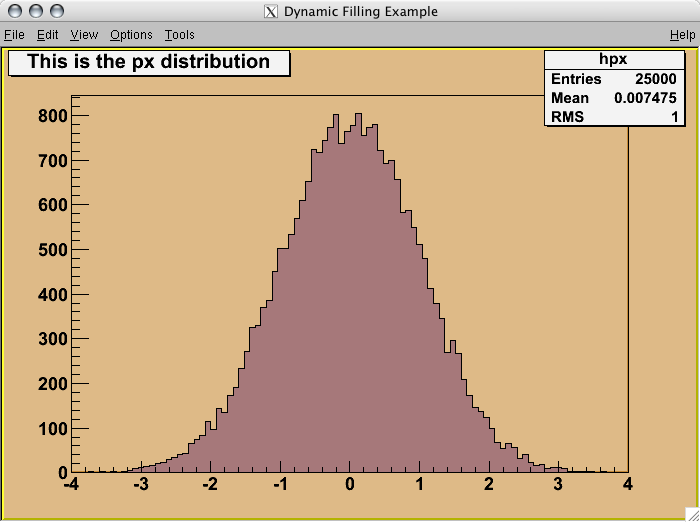
\includegraphics[width=12cm]{fig/hsimple.png}
  \caption{hsimpleの実行結果}
  \label{fig:hsimple}
\end{figure}

もし、あなたのアカウントが\texttt{\$ROOTSYS/tutorials}に書き込み権限を持たない場合、\texttt{hsimple.root}を開けないというエラーが出るでしょう。そのような場合は、書き込み権限を持つユーザで作業をするか、\texttt{\$ROOTSYS/tutorials}をディレクトリごと自分のホームディレクトリの下にコピーして、そこで作業をしましょう。

\section{ROOTの操作に慣れる}

まずは、簡単な例を走らせることでROOTの操作方法に慣れましょう。ここでは、標準偏差(standard deviation)$\sigma=1$の正規分布(normal distribution、Gaussian distribution)に従った、標本の大きさ(sample size)$n=10000$のヒストグラム(histogram)を作ってみます。

\subsection{コマンドラインからの操作}
まずはROOTを起動し、
\begin{lstlisting}[language=c++]
root [0] TH1D* hist = new TH1D("myhist", "Gaussian Histogram (#sigma = 1)", 50, -5, 5)
root [1] hist->FillRandom("gaus", 10000)
root [2] hist->Draw()
Info in <TCanvas::MakeDefCanvas>:  created default TCanvas with name c1
\end{lstlisting}
という3行を打ってみて下さい。最後の行はROOTが自動的に出力しますが、エラーではないので今は気にしないで下さい。図\ref{fig:first_script}のような実行結果が画面に現れます。
\begin{figure}
  \centering
  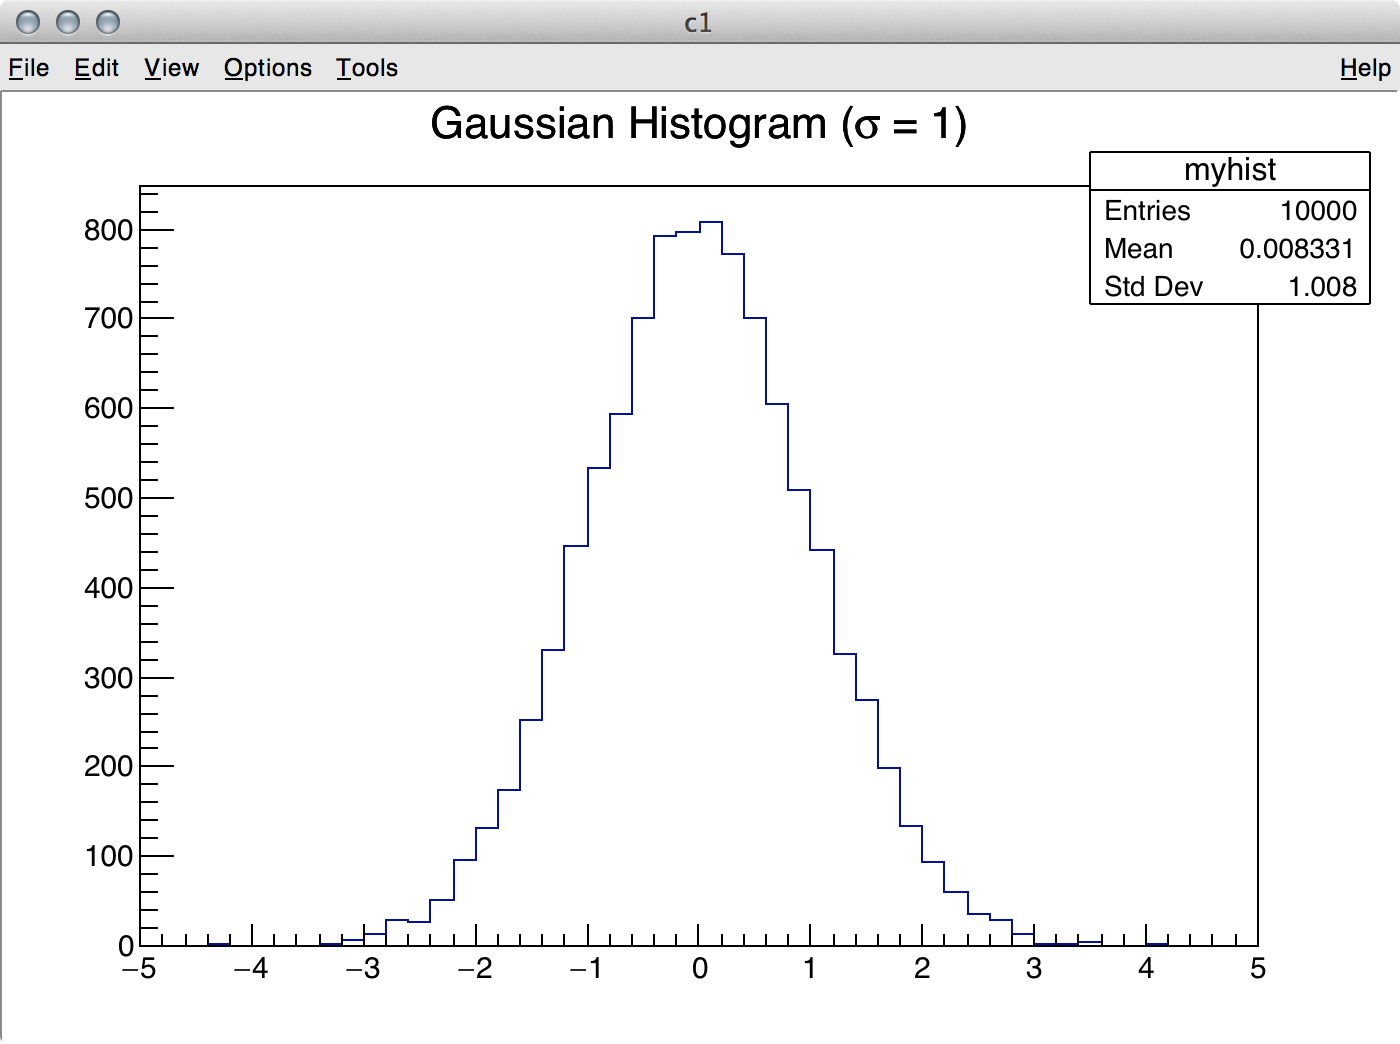
\includegraphics[width=12cm]{fig/first_script.png}
  \caption{標準偏差$\sigma=1$、標本の大きさ$n=10000$のヒストグラム}
  \label{fig:first_script}
\end{figure}

このままでは何が起きたか分からないので、簡単に説明します。C++やプログラミングの用語が混ざりますが、各自で調べつつ読んで下さい。これらの3行は、実はC++の言葉で書かれています。まず
\begin{lstlisting}[language=c++]
root [0] TH1D* hist = new TH1D("myhist", "Gaussian Histogram (#sigma = 1)", 50, -5, 5)
\end{lstlisting}
の部分では、\texttt{TH1D}クラス(class)のインスタンス(instance)を作成しています。このインスタンスの名前は、この例ではhistとしています。\texttt{*}や\texttt{new}は、おまじないだと思っておいて下さい\footnote{コンピュータ関連の説明文書の中で、「おまじない」という言葉がたまに出てきます。「それが何者であるか(今は)理解する必要はないが、こうしておくと正しく動作する」ようなものを「おまじない」と呼ぶ習慣があります。とりあえず気にするなということです。}。このhistが、ヒストグラムの実体になります。\texttt{"myhist"}や\texttt{"Gaussian Histogram (\#sigma = 1)"}という文字列、$50$、$-5$、$5$という数字が図\ref{fig:first_script}のどの箇所に対応するか、自分で考えて下さい。このヒストグラムは、この時点では作りたてなので、当然中身は空っぽです。そこで
\begin{lstlisting}[language=c++]
root [1] hist->FillRandom("gaus", 10000)
\end{lstlisting}
として、正規分布に従う数字$10000$個を乱数で発生させ、ヒストグラムに詰めています。最後に
\begin{lstlisting}[language=c++]
root [2] hist->Draw()
\end{lstlisting}
としてヒストグラムを画面に描画させています。

ROOT プロンプトで入力したコマンドは、\texttt{.q} や \texttt{.x} のような ROOT 固有のコマンドをのぞいて基本的には C++ の文法で記述する必要があります。しかし利便性を高めるためにいくつか C++ とは異なる文法でも動作するようになっています。C や C++ を既に知っている読者の場合、この節で取り上げた例の各行にセミコロン \texttt{;} がないことに気がつくかもしれません。次の例のように、ROOT プロンプトではセミコロンの有無で表示が変わります。スクリプトファイルに書く際は、セミコロンを忘れないようにしてください。

\begin{lstlisting}[language=c++]
root [0] int a = 1
(int) 1
root [1] int b = 2;
root [2] 
\end{lstlisting}

\subsection{スクリプトを使った操作}
今回の例はたったの3行ですので入力は簡単です。しかし、このようなヒストグラムを何百回と繰り返し作成することを想像してみて下さい。実際のデータ解析では、取得した大量のデータに同じ処理をしたい場合があります。そのようなときに、同じコマンドを何度も繰り返し入力するのは非効率的です。そこで、先ほどの3行を1つのファイルにまとめて書いてしまいましょう。コード\ref{code:first_script}の内容を入力したテキストファイルを\texttt{first\_script.C}というファイル名で好きな場所に保存して下さい\footnote{日本語の文章の書き方は個人で色々な癖があるように、プログラミング言語の記述にも人それぞれの流儀があります。本書で採用しているコードの流儀は、かなり著者の好みが反映されています。}。このようなファイルを、ROOTのスクリプトファイル、マクロファイルなどと呼びます。
%\begin{NoFloat}
\lstinputlisting[language=c++,float=tb,caption=\texttt{first\_script.C},label=code:first_script,numbers=left]{src/first_script.C}
%\end{NoFloat}

\texttt{first\_script.C}を保存したディレクトリに移動し、その場所でROOTを立ち上げ、次の行を実行します。
\begin{lstlisting}[language=c++]
root [0] .x first_script.C
Info in <TCanvas::MakeDefCanvas>:  created default TCanvas with name c1
\end{lstlisting}
先ほどと同様の実行結果(図\ref{fig:first_script})が得られるはずです。ここで、再び\texttt{.x}というコマンドが登場しました。\texttt{first\_script.C}を実行せよという意味です。\texttt{first\_script.C}に書かれた内容が逐一実行されたため、図\ref{fig:first_script}の結果が得られたわけです。

1度実行するだけでは、せっかく別ファイルにしたありがたみが分かりません。そこでコード\ref{code:first_script2}のように少し書き直して、\texttt{first\_script2.C}というファイルを作成してみて下さい。
%\begin{NoFloat}
\lstinputlisting[language=c++,float=tb,caption=\texttt{first\_script2.C},label=code:first_script2,numbers=left]{src/first_script2.C}
%\end{NoFloat}
先ほどと同様に実行してみましょう。ただし今回は
\begin{lstlisting}[language=c++]
root [0] .x first_script2.C(500, 100000)
Info in <TCanvas::MakeDefCanvas>:  created default TCanvas with name c1
\end{lstlisting}
としてみます。少し先ほどの例とは表示されるヒストグラムが変化したはずです。2つの数字を何通りか試して、何が起きてるか確かめて下さい。何度も実行すると、
\begin{lstlisting}[language=c++]
Warning in <TROOT::Append>: Replacing existing TH1: myhist (Potential memory leak).
\end{lstlisting}
というROOTの警告(warning)が出るはずですが、今は無視しましょう。

ここまでの作業を振り返ってみます。最初にROOTのプロンプトから入力した行は3行だけでしたが、コード\ref{code:first_script}と\ref{code:first_script2}では上に2行、下に1行追加され、合計6行になっています。この余計な部分を含めて、関数(function)と呼びます。\texttt{void}は、その関数が値を返さないという意味です。\texttt{int nbins}や\texttt{int nevents}の部分は、引数(argument)と呼ばれるものです。このように特定の機能を関数化することによって、汎用性が高くなります。

ROOTのスクリプトファイルでは、そのファイル名と同一の関数がファイル内に存在すると、その関数が実行されます。したがって、コード\ref{code:first_script2}に書いた関数名を\texttt{first\_script2}から例えば\texttt{foo}\footnote{\texttt{foo}や\texttt{bar}というのは、とりあえずの適当な名前として、プログラミングの話題をするときによく出てきます。日本語だと、「ほげ」や\texttt{hoge}という単語もよく使われます。}に変更してしまうと、
\begin{lstlisting}[language=c++]
root [0] .x first_script2.C(500, 100000)
warning: cannot find function 'first_script2()'; falling back to .L
\end{lstlisting}
というエラーが出てヒストグラムが表示されません。もしファイル名と関数名を別々のものにしたければ、次のやり方も可能です。
\begin{lstlisting}[language=c++]
root [0] .L first_script2.C
root [1] foo(500, 100000)
Info in <TCanvas::MakeDefCanvas>:  created default TCanvas with name c1
\end{lstlisting}
\texttt{.L}コマンドで\texttt{first\_script2.C}をロード(LoadのL)します。そのスクリプトファイルの内容をROOTが呼び出せるようにする作業のことです。\texttt{first\_script2.C}は既にロードされましたので、その中に書かれていた関数\texttt{foo}に引数を与えて直接呼び出すことができます。また、ひとつのスクリプトの中に複数の関数を記述しても問題ありません。ロードした後に、好きな関数を呼び出して下さい。
\subsection{図を保存する}

図\ref{fig:hsimple}や\ref{fig:first_script}の例は、筆者の使用しているmacOS上でスクリーンショットを撮ったものです。論文用の図を作成する場合は、ウインドウ上のリサイズボックスやタイトルバーは必要ありません。\LaTeX\ 文書で一般的に使われる、PDF形式で出力結果を保存してみましょう\footnote{最近の\LaTeX\ 環境では\texttt{latex}コマンドよりも\texttt{pdflatex}コマンドを使用してPDFファイルを生成するのが一般的になりつつあります。そのため、論文出版社もEPS形式ではなくPDF形式で図を受け付けています。またEPSよりもPDFのほうがパソコン上での閲覧も楽なため、特に理由がない場合はPDFで保存しましょう。ただし、本書のような日本語文書では\texttt{platex}コマンドがまだまだ使われています。}。\texttt{first\_script.C}の実行結果が表示されたら、ウインドウ左上にある「File」メニューから「Save As\ldots」を選択し、好きな場所に好きな名前で出力結果を保存しましょう。図\ref{fig:first_script_pdf}は、この手順で図\ref{fig:first_script}をPDF形式で保存し直したものです。このPDF文書を拡大しても、図が綺麗なことが分かります。いくつか保存形式が選べますので、試してみましょう。JPEG形式は図の細部が潰れますので、絶対に使わないでください。ウェブページに掲載する目的などでビットマップ画像が必要な場合は、PNG 形式(.png)にしてください。GIF形式は最大で256色までしか使用できないので、画面で見ている色と変わってしまう可能性があります。

\begin{figure}
  \centering
  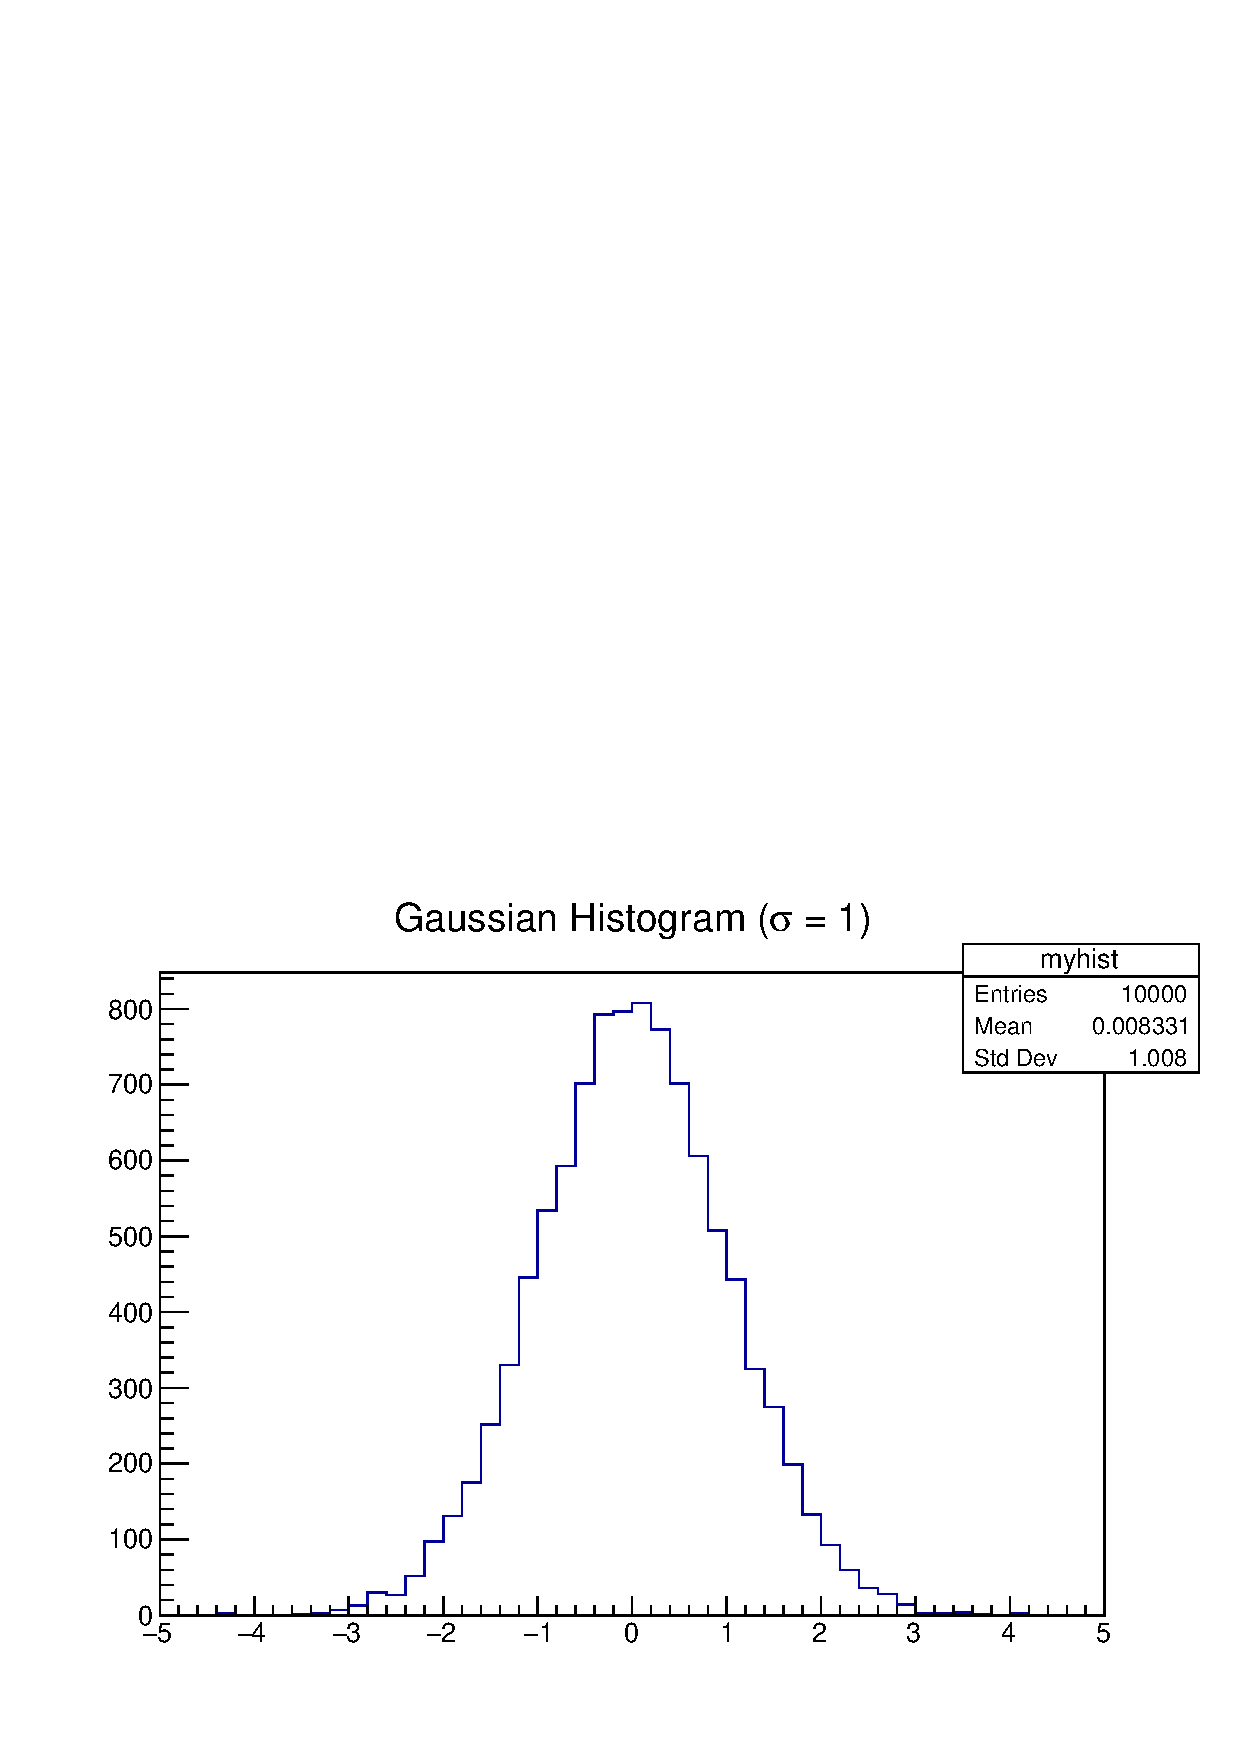
\includegraphics[width=12cm,clip]{fig/first_script_pdf.pdf}
  \caption{図\ref{fig:first_script}を、PDF形式で保存し直したもの。拡大しても細部まで滑らかなことが分かる。}
  \label{fig:first_script_pdf}
\end{figure}

メニューからいちいち保存するのは面倒ですので、スクリプトを実行したらキャンバスをプロンプトから PDF で保存してみましょう。

\begin{lstlisting}[language=c++]
root [0] .x first_script.C
Info in <TCanvas::MakeDefCanvas>:  created default TCanvas with name c1
root [1] c1->SaveAs("his.pdf")
Info in <TCanvas::Print>: pdf file hist.pdf has been created
\end{lstlisting}

ROOT の生成する横長の PDF には\texttt{/Rotate 90}というタグが含まれています。\texttt{dvipdfmx}コマンド\footnote{TeX Live 2018 以降では問題ありません。}や Apple Keynote の古いバージョンなどでこれを正常に処理できないことがあり、そのため作成した PDF が90度回転して表示されるという問題があります(ROOTの問題ではありません)。これを回避するためには、横長の図の場合に\texttt{c1->SaveAs("hist.pdf")}などと実行するのではなく、\texttt{c1->Print("hist.pdf", "pdf Portrait")}と実行しましょう。

\begin{lstlisting}[language=c++]
root [1] c1->Print("hist.pdf", "pdf Portrait")
Info in <TCanvas::Print>: pdf file hist.pdf has been created
\end{lstlisting}

\subsection{タブ補完を使う}
ROOTのプロンプトでコマンドを打つ場合、キーボードのタブキーを押すことで、補完することができます。携帯電話の文字入力の予測変換機能のようなものです。例えば、
\begin{lstlisting}[language=c++]
root [0] TH1D* hist = new TH1D("myhist", "Gaussian Histogram (#sigma=1)", 50, -5, 5)
root [1] hist->FillRandom("gaus", 10000)
root [2] hist->Draw()
Info in <TCanvas::MakeDefCanvas>:  created default TCanvas with name c1
root [3] hi
\end{lstlisting}
とまで入力したところで、タブキーを押してみましょう。自動的に
\begin{lstlisting}[language=c++]
root [3] hist
\end{lstlisting}
と補完されます。次に、
\begin{lstlisting}[language=c++]
root [3] hist->Get
\end{lstlisting}
まで入力して再度タブを押してみましょう。次のような候補が大量に現れるはずです。
\begin{lstlisting}[language=c++]
GetArray
GetAsymmetry
GetAt
GetAxisColor
\end{lstlisting}
これは、インスタンス\texttt{hist}に操作可能な機能のうち、\texttt{Get}で始まるものの一覧です。C++の言葉で言い換えると、クラス\texttt{TH1D}のメンバ関数(member function)のうちゲッター(getter)の一覧です。候補を眺めてみると、\texttt{GetMean}や\texttt{GetStdDev}\footnote{\texttt{GetRMS}というメンバ関数も見つかると思います。ROOTやPAWで「RMS」と言った場合、これは二乗平均ではなく標準偏差を指します。統計学の用語としては不適切なのですが、歴史的理由でRMSという言葉を使い続けていたそうです(PAW で間違って使ってしまった用語との互換性を保つため、ROOT でもわざと間違った用語を使い続けた)。そのためこの業界ではRMSという用語を間違って覚えている人が沢山いますが、優しく注意してあげて下さい。最近のROOTでは、\texttt{GetRMS}と全く同じ働きをする関数として\texttt{GetStdDev}が用意されており、後者が本体です。}というメンバ関数が見つかるはずです。何をする関数か、一目瞭然でしょう。それでは
\begin{lstlisting}[language=c++]
root [3] hist->GetMe
\end{lstlisting}
まで打ち、タブキーを押しましょう。
\begin{lstlisting}[language=c++]
root [3] hist->GetMean
GetMean
GetMeanError
\end{lstlisting}
の2候補にまで絞られます。今は\texttt{GetMean}を試したいので、
\begin{lstlisting}[language=c++]
root [3] hist->GetMean(
\end{lstlisting}
とまで打って再度タブを打ちましょう。今度は、
\begin{lstlisting}[language=c++]
Double_t GetMean(Int_t axis = 1) const
\end{lstlisting}
と表示されます。これは、\texttt{TH1D::GetMean}\footnote{この書き方は、クラス\texttt{TH1D}のメンバ関数\texttt{GetMean}という意味です。}の引数の説明が表示されたものです。引数には整数(integer)値を取り、そのデフォルト(default)値が1だという意味です(1はX軸を意味しています)。何も打たなくてもX軸を指定するデフォルト値が入っているので、
\begin{lstlisting}[language=c++]
root [3] hist->GetMean()
(Double_t) 0.00833117
\end{lstlisting}
と入力します。出力された値は、このヒストグラムの平均値です。ウインドウの右上に既に表示されている値と同一なはずです。同様にして、\texttt{TH1D::GetStdDev()}も試してみましょう。

今度は
\begin{lstlisting}[language=c++]
root [4] hist->Set
\end{lstlisting}
でタブ補完をすると、\texttt{Set}で始まる関数がたくさん表示されます。これらのメンバ関数はセッター(setter)と呼ばれ、ゲッターと対をなすものです。ゲッターとセッター以外にも多くのメンバ関数が存在しますが、ここでは説明しません。試しに
\begin{lstlisting}[language=c++]
root [4] hist->SetLineColor(2)
root [5] hist->SetXTitle("x")
root [6] hist->SetYTitle("Number of Events")
root [7] hist->Draw("e")
\end{lstlisting}
としてみましょう。出力結果と見比べて、何が起きたか分かるはずです。先ほどまでは\texttt{TH1D::Draw}の引数に何も与えていませんでしたが、今度は\texttt{"e"}という引数がついています。なぜこれで動作したかというと、これも、引数のデフォルト値が存在していたためです。
\begin{lstlisting}[language=c++]
root [8] hist->Draw(
\end{lstlisting}
でタブキーを押して、意味を理解して下さい。\texttt{first\_example.C}の中の関数\texttt{first\_example}では、引数のデフォルト値を設定していません。そのため引数を必ず両方とも指定しないと正しく動作しません。

\section{やっておきたい初期設定}

コード\ref{code:rootlogon}を、\texttt{\~{}/.rootlogon.C}として保存して、再度ROOTを起動しましょう\footnote{コード\ref{code:first_script}では、\texttt{hist}というインスタンス(のポインタ)を自分で作りました。しかし、\texttt{gROOT}や\texttt{gStyle}というインスタンスは作った記憶がありません。これはROOTが内部的に既に持っている、グローバル(global)インスタンスです。}。その名が示す通り、ROOTを起動したとき(ログオンしたとき)に読み込まれるファイルです。再び\texttt{first\_script.C}を走らせると、図\ref{fig:first_script_mod_eps}のような結果が得られます。まだまだ見栄えを変更可能ですが、ひとまずは良しとします。もし図\ref{fig:first_script_pdf}のほうが好みであれば、コード\ref{code:rootlogon}の不要な行を消していきましょう。どんな設定項目があるかは、\url{http://root.cern.ch/root/html/TStyle.html}を参照して下さい。

学会の発表資料では太い文字のほうが可読性が高いので、デフォルトのフォント(Helvetica)のままでも良いでしょう。ただし、ヒストグラムのタイトル部分を見ると「$\sigma$」と他の文字のフォントが一致していません。このように数式を文字列中に組み込むとゴシック体では格好悪いので、好みによってTimesに変更します。

\begin{NoFloat}
\lstinputlisting[language=c++,float=tb,caption=\texttt{.rootlogon.C}の例,label=code:rootlogon]{src/rootlogon.C}
\end{NoFloat}
\pagebreak

\begin{figure}
  \centering
  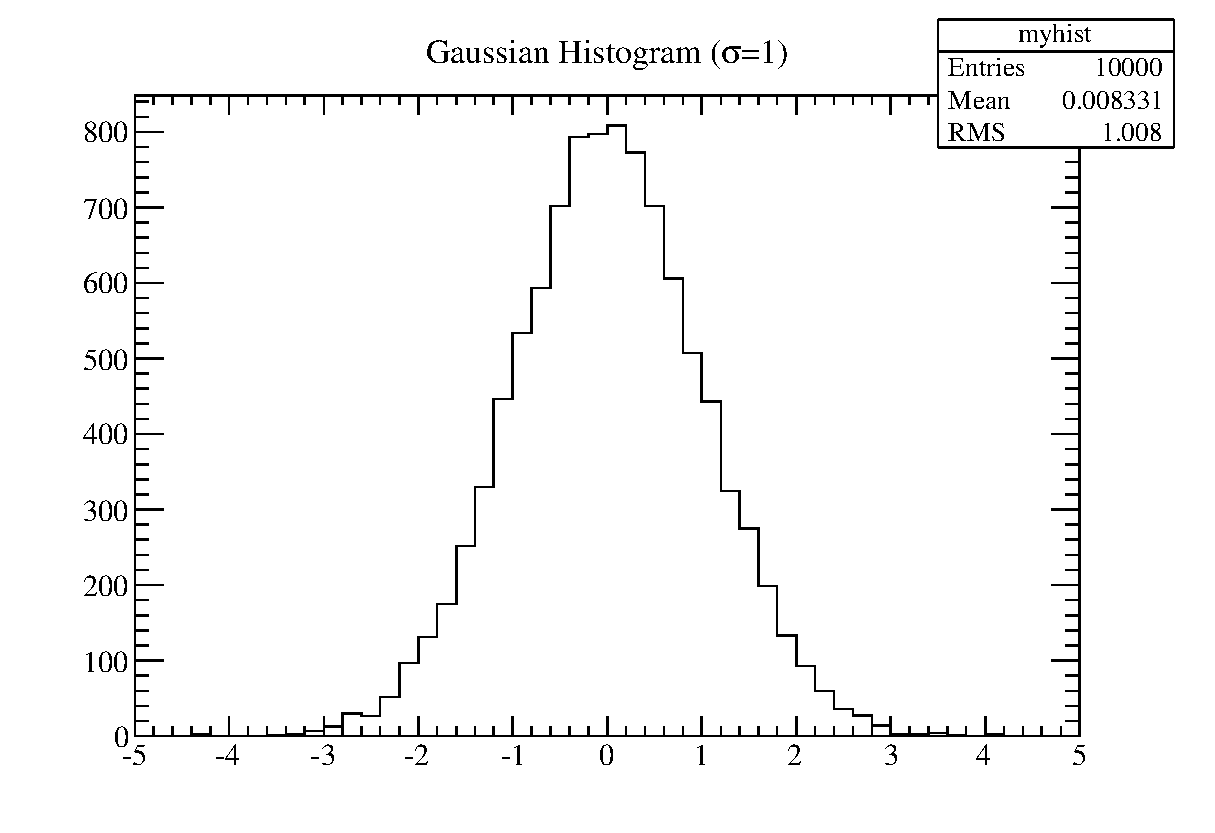
\includegraphics[width=12cm,clip]{fig/first_script_mod.eps}
  \caption{\texttt{\~{}/.rootlogon.C}を使って図\ref{fig:first_script_pdf}の見栄えを変更したもの}
  \label{fig:first_script_mod_eps}
\end{figure}

ひとつ注意して欲しいのが、あなたの画面で見えている色の設定は、万人に同じように見えるわけではないということです。人間は色覚特性というものを持ち、例えば赤と緑の区別が困難な人も存在します。またパソコンの液晶ディスプレイで見えている状態と、学会会場のプロジェクタで映される色はコントラストが異なるため、明るい黄色や黄緑は認識しにくくなります。さらに白黒印刷した場合には、カラー印刷とは全く違う見え方をします\footnote{紙媒体の雑誌は多くのページが白黒印刷であり、また科研費や学振特別研究員の申請書は白黒印刷で審査員に送付されます。}。そのため、なんでもかんでも好きな色に設定して良いわけではありません。どのような色覚特性であっても、どのような会場でも、どのような印刷方法でも色や線の区別をつけられるように心がけましょう。

\emphasize{ROOT 5.30より古いバージョン}を使っている場合、図\ref{fig:first_script_pdf}の背景色が薄い灰色になります。これでは通常の論文で使用するには問題があります。研究室内のみで使うような図だとしても、プリンタのインクの無駄ですので、次の設定を追加してください。

\begin{lstlisting}[language=c++]
gROOT->SetStyle("Plain"); // Set the overall design to "Plain" mode
gStyle->SetTitleBorderSize(0); // Remove the boarder from title panels
gStyle->SetFrameFillColor(0); // Set the frame color to white
gStyle->SetCanvasColor(0); // Set the canvas color to white
gStyle->SetPalette(1); // Rainbow color palette
\end{lstlisting}


\chapter{C++の基礎}
\label{chapter_C++}

この章では、プログラミングやC++の初心者向けに、C++の簡単な解説を行います。第\ref{chapter_Install}章の内容や用語がチンプンカンプンだった人は、この章を読んでから先に進むのが良いでしょう。筆者が重要だと思う箇所だけを抜粋して解説しますので、網羅的なC++の解説書も参照することをお勧めします。

ただし、いきなり一般書籍を購入しても当たり外れがあります。特に、C++と銘打っていても、コードの書き方の癖がC言語に近い書物はやめたほうが無難です\footnote{C++の入門書ではありませんが、『Numerical Recipes in C++』は悪書の例です。}。例えば
\begin{lstlisting}[language=c++]
int i;
for (i = 0; i < 100; i++) {
  // some codes...
}
\end{lstlisting}
のように書かれている本よりも
\begin{lstlisting}[language=c++]
for (int i = 0; i < 100; i++) {
  // some codes...
}
\end{lstlisting}
と書かれている本を選んで下さい。また、なるべくクラス(class)の概念が早めに登場する本が良いでしょう。いきなり一般書籍を読み進める前に、まずは本書を眺めてC++言語やプログラミングとは何かを掴んで下さい。プログラミングの専門家を目指すわけではないので、研究室では「使って覚える」を実践するべきです。インターネット上で日本語で閲覧可能なものでは、以下の2つをお勧めします。
\begin{itemize}
\item C++入門\\
\url{http://www.asahi-net.or.jp/~yf8k-kbys/newcpp0.html}
\item ATLAS Japan C++ Course\\
\url{http://www.icepp.s.u-tokyo.ac.jp/~sakamoto/education/atlasj/cplusplus/index.html}
\end{itemize}
この他にも「C++ 入門」などでインターネットを検索すれば大量に出てきますので、好みに合うものを選択してください。

C++が分かればROOTは理解しやすいのですが、ユーザの利便性を考えて、ROOTには独自の仕様が存在します。このような両者の違いについても、この章では説明します。 
\clearpage
\section{Hello World!}
%\begin{NoFloat}
\lstinputlisting[language=c++,float=tb,caption=\texttt{hello\_world.cxx},label=code_hello_world,numbers=left]{src/hello_world.cxx}
%\end{NoFloat}
まず好きなエディタを使って、コード\ref{code_hello_world}を\texttt{hello\_world.cxx}というファイル名で保存して下さい\footnote{Emacs、vi、gedit、TextEditなど何でも構いません。}。次にターミナルから、
\begin{lstlisting}[language=bash]
$ g++ hello_world.cxx
$ ./a.out
\end{lstlisting}
と打ちます\footnote{もし\texttt{g++}が見つからないという内容のエラーが出たら、お使いのコンピュータにGCCをインストールして下さい。「Scientific Linux GCC intall」「OS X GCC intall」などで検索すれば方法は見つかるはずです。Scientific Linux の場合は\texttt{yum}コマンドを使ってGCCを入れることができます。またOS Xの場合はXcodeをAppleからダウンロードしてインストールして下さい。}。
\begin{lstlisting}
Hello World!
\end{lstlisting}
と表示されるはずです。この一連の作業は、
\begin{enumerate}
  \item あなたが\texttt{hello\_world.cxx}というプログラムをエディタで作成し
  \item あなたが\texttt{g++}というコマンド\footnote{GNU Compiler Collection(GCC)に含まれる、C++用のコンパイラです。}に\texttt{hello\_world.cxx}をコンパイルするように指示を出し
  \item \texttt{g++}が\texttt{hello\_world.cxx}をコンピュータが実行できるファイル\texttt{a.out}に変換し
  \item あなたが\texttt{a.out}を実行し
  \item 「Hello World!」という文字列が出力された
\end{enumerate}
ということです。これがプログラミングをするという作業の基本的な流れです。

\texttt{a.out}という変な名前は、\texttt{g++}が作成する実行ファイルのデフォルトの名前です。いくつもプログラムを作成したら、区別できなくなってしまいます。そこで\texttt{g++}に引数をつけて
\begin{lstlisting}[language=bash]
$ g++ hello_world.cxx -o hello_world
$ ./hello_world
\end{lstlisting}
とすれば、好きな名前で実行ファイルを作成してくれます。

さて、コード\ref{code_hello_world}の解説です。まずこのプログラムは、「Hello World!」と呼ばれる、初心者の解説向けによく用いられるものです\footnote{\url{http://ja.wikipedia.org/wiki/Hello_world}などに解説あり。}。このプログラムの主な作業は
\begin{lstlisting}[language=c++]
  printf("Hello World!\n");
\end{lstlisting}
の部分が担っています。\texttt{printf}という関数(function)を使って、「Hello Wolrd!」という文字列を出力させています\footnote{C++では\texttt{std::cout}を紹介するべきですが、ROOTの\texttt{Form}関数やPythonの文字列操作で\texttt{printf}に近い操作が出てくるため、あえて\texttt{printf}を使っています。}。日本語で「関数」と言うと、普通は$y=f(x)$のような数学の関数を想像するでしょう。しかしプログラミングの世界の関数は、必ずしも数字を扱うものではありません。「function」という単語は「機能」という訳語も持ちます。特定の機能をもった命令の集まりが関数です。

\texttt{printf}という名前には、意味があります。「print」という単語と「format」という単語を組み合わせたものです。文字列の書式を整えて出力する関数なので\footnote{この書式の機能は今は使っていません。}、このような名前になっています。関数の名前は、何をする機能を持っているか分かるようになっていなくてはなりません。数学では$y=f(x)$、$y=g(x)$のように抽象的な名前を使いますが、プログラムの中で
\begin{lstlisting}[language=c++]
  g("Hello World!\n");
\end{lstlisting}
と書かれていては、可読性が悪くなります。

さて、「\textbackslash n」という2文字は何でしょうか。これは改行を表す特殊文字です。2文字で1文字だと考えて下さい。試しにコード\ref{code_hello_world}から「\textbackslash n」を取り除いてコンパイルし、実行してみて下さい。改行の有無で出力結果が変わります。

この「Hello World!」という文字列のことを、\texttt{printf}に渡した引数(ひきすう、argument)と言います\footnote{文字列は常に二重引用符で囲む必要があります。二重引用符自体を文字列の中で使用する場合には、\texttt{"\textbackslash ""}のように、バックスラッシュを前方に置きます。}。好きな文字列を渡すことによって、出力結果が変わります。「Hello World!」という文字列しか出力できない関数を作るのではなく、このように引数を変更することで結果を変更できるのが、関数を用意することの最大の利点です。

それではなぜ、この\texttt{printf}という関数を我々は使うことができるのでしょうか。その答えはコード\ref{code_hello_world}の先頭にあります。この行はインクルード(include)文と呼ばれ、他のファイルに既に存在している\texttt{printf}を見えるようにしています\footnote{\texttt{cstdio}は「C」、「standard」、「input/output」の合成語です。C言語の時代に作られた、標準入出力のためのライブラリです。}。したがって、この箇所を
\begin{lstlisting}[language=c++]
// #include <cstdio>
\end{lstlisting}
のようにコメントアウト(comment out)\footnote{先頭が「//」で始まる行は、全てコンパイラに無視されます。}してコンパイルすると、
\begin{lstlisting}[language=bash]
$ g++ -Wall hello_world.cxx
hello_world.cxx: In function ‘int main()’:
hello_world.cxx:5: error: ‘printf’ was not declared in this scope
\end{lstlisting}
とエラーを吐きます。コンパイラは\texttt{printf}が一体なんなのか分からなくなるわけです。

このエラーメッセージを読むと、「In function `int main()'」と書かれています。そうです、この\texttt{main}というのも関数です。この関数のことを\texttt{main}(メイン)関数と呼びます。\texttt{main}関数は、プログラム中に必ず存在しなくてはいけません。\texttt{main}関数の中に書かれた内容が、プログラムの実行時に呼び出される決まりになっているからです。「関数の中」とは\texttt{\{}から\texttt{\}}の中を指しています。この括弧を書くことで、コンパイラは\texttt{main}関数の範囲を理解できるようになります。

\texttt{main}の前にある\texttt{int}(integerのint)は、\texttt{main}関数の返り値(return value)の型(type)を示しています。一般的に、関数は呼び出されると何か値を返します。数学の二次関数$y=f(x)=ax^2+bx+c$であれば、関数$f$に$x$という値を入れると、$ax^2+bx+c$を返しますね。これと同じです。\texttt{main}関数の返り値は、必ず整数(integer)でなくてはいけません。この返り値が0であれば、\texttt{main}関数が正常終了したということを示します。最後に
\begin{lstlisting}
  return 0; 
\end{lstlisting}
と書くことで、確かに\texttt{0}を返す設計になっています。返り値は、\texttt{return}を使って返すことができます。もしこれを\texttt{0}ではなく\texttt{-1}などにすれば、このプログラムは異常終了したとOS側が判断します。

\section{型と関数}
\label{sec:型と関数}
前節の説明では、型、関数、引数、返り値という用語がでてきました。ここでは、もう少し例を挙げて説明します。コード\ref{code_triple}を作成してコンパイルし、実行してみましょう。
%\begin{NoFloat}
\lstinputlisting[language=c++,float=tb,caption=\texttt{triple.cxx},label=code_triple,numbers=left]{src/triple.cxx}
%\end{NoFloat}
15という整数値を持つ変数(variable)\texttt{before}を
\begin{lstlisting}
  int before = 15; 
\end{lstlisting}
のようにして作成しています。数学の変数は、その中身をいつでも整数や無理数や複素数に変更できます。しかしC++の場合は、その変数の種類を後から変更できません。変数\texttt{before}の中身は、いつでも整数値です。先頭の\texttt{int}は、変数\texttt{before}が常に整数値を持つという意味です。これを型(type)と呼びます。つづいて\texttt{= 15}というのが出てきますが、これは「\texttt{before}に15を代入する」という意味です。「\texttt{before}と15は等しい」という意味ではありません。ここは、数学の等号と使用方法が異なります。もしこの直後に
\begin{lstlisting}[language=c++]
before = before * before + 1;
\end{lstlisting}
という文を足すと、\texttt{before}の値が226に変更されます。\texttt{before}の値が二次方程式$x=x^2+1$の解に自動的に変更されたりはしないのです。C++の\texttt{=}は、数学の等号ではなく代入を表します。

関数\texttt{triple}は、引数に与えられた整数値\texttt{v}を、3倍して返す関数です\footnote{C++では、四則演算の記号$+$、$-$、$\times$、$\div$はそれぞれ\texttt{+}、\texttt{-}、\texttt{*}、\texttt{/}で表します。}。整数を3倍してもやはり整数なので、返り値は\texttt{int}になっています。このような関数を作ってしまえば、
\begin{lstlisting}[language=c++]
  int after = triple(before);
\end{lstlisting}
として変数\texttt{after}に関数の返り値を代入することができます。この右辺が呼ばれると、処理は関数\texttt{triple}の行に飛び、
\begin{lstlisting}[language=c++]
  return 3 * v;
\end{lstlisting}
で値が返されて、左辺に代入されます。

そして最後に、変数\texttt{before}、\texttt{after}の中身を
\begin{lstlisting}[language=c++]
  printf("Before: %d\n", before); 
  printf("After : %d\n", after);
\end{lstlisting} 
で出力させています。ここでは、\texttt{printf}の「format」の機能を利用しています。\texttt{\%d}という文字列は、intの変数を文字列に整形して出力するという意味です。\texttt{printf}はこのように、複数の引数(可変長引数)を取ることが可能です。

\texttt{int}以外にも、C++には何種類か型があります。代表的なものが、\texttt{double}(ダブル)です。\texttt{double}型は、\texttt{int}と異なり小数を使うことができます。なぜ\texttt{double}という名前かと言うと、同じように小数を扱う型に\texttt{float}(フロート)があるからです。\texttt{double}は\texttt{float}に比べてメモリを2倍(double)消費します。しかしその分、精度がよくなります\footnote{C++で扱われる小数には精度がつきまといます。例えば$\frac{3}{2}$を小数に直すと、どれだけ小さいほうの桁を見ても0が続きます。しかしコンピュータ上にこのような無限の精度を持つ数を定義すると、メモリが無限大必要になります。これでは実現不可能なため、ある程度の精度を犠牲にします。例えば円周率を\texttt{double}型で扱いたい場合には、有効桁数が15桁しかありません。 $3.14159265358979$までしか精度が保証されないのです。\texttt{float}にした場合はさらに精度が下がり、7桁しか有効桁数がありません。したがって、$1.3\times10^{20}$と$3.4\times10^{-13}$の引き算をそのままC++で実行しても、数学的に正しい数字は得られないので注意が必要です。}。

さて、コード\ref{code_triple}の例では、\texttt{triple}関数は引数と返り値が\texttt{int}型でした。もし\texttt{before}の値が$16.9$だとすれば、\texttt{after}の値は期待通りに動作しません。そこで引数と返り値を\texttt{double}に変更したものを追加したのが、コード\ref{code_triple2}です。同名の\texttt{triple}関数が2つありますが、片方は\texttt{int}用で片方は\texttt{double}用です。このように同じ名前の関数に対して、異なる引数を与えることで処理内容を変更することを、関数のオーバーロード(overload)と言います。コンパイラが引数の違いを適切に見つけ出し、異なる処理をしてくれます。

%\begin{NoFloat}
\lstinputlisting[language=c++,float=tb,caption=\texttt{triple2.cxx},label=code_triple2,numbers=left]{src/triple2.cxx}
%\end{NoFloat}

コード\ref{code_triple2}はコード\ref{code_triple}と違い、\texttt{main}の前に実体を伴わない2つの関数が書かれています。これは関数の前方宣言(forward declaration)と呼ばれるものです。今はなくても構いませんが、ヘッダーファイルを分割して書くようになるときには必須の作業です。このように返り値と引数だけ先に書いておくことで、実際の関数の中身を知らなくても(関数が後で定義されていても)、コンパイラは\texttt{main}関数の中で\texttt{triple}が出てきても問題なく処理を続行できるようになります。プログラムの可読性を高めるという意味もあります。\texttt{main}関数の後に、実際の\texttt{triple}関数の中身が記述されています。これを、関数の定義(definition)と呼びます。

新たな\texttt{printf}の使い方として、
\begin{lstlisting}[language=c++]
  printf("Before: %f\n", before_d); 
  printf("After : %f\n", after_d); 
\end{lstlisting} 
のように\texttt{\%d}ではなく\texttt{\%f}というのが登場しています。これは、\texttt{double}型を整形するための特殊な文字列です\footnote{他にもフォーマットの種類がいくつか存在しますので、「\texttt{printf}」で検索してみてください。}。

なぜこれらの例で、2倍にする関数ではなく3倍にするものを選んだかというと、\texttt{double}という単語がC++の予約語(reserved word)だからです。C++が既に確保している名前を、ユーザが勝手に使うことはできません。\texttt{printf}のように一般的に使われる関数名も、使わないことが推奨されます。もしあなたが「f」という文字を出力する関数を\texttt{printf}という名前で作成したら、他の人は混乱するでしょう。

\section{\texttt{if}文と関係演算子}

ここまでで、関数の簡単な使い方が分かりました。しかし、四則演算程度しかまだやり方をしりません。2つの数字の大小を比べるにはどうしたら良いでしょうか。この節では、関係演算子と\texttt{if}文の使い方を説明します。

%\begin{NoFloat}
\lstinputlisting[language=c++,float=tb,caption=\texttt{minmax.cxx},label=code_minmax,numbers=left]{src/minmax.cxx}
%\end{NoFloat}

コード\ref{code_minmax}には、新しい関数\texttt{min}と\texttt{max}を作りました。初めて、
\begin{lstlisting}[language=c++]
  if (v1 < v2) {
    ret = v1;
  } else {
    ret = v2;
  }
\end{lstlisting}
という\texttt{if}文が出てきます。これを日本語訳すると、「もし(\texttt{if})\texttt{v1}が\texttt{v2}よりも小さければ、\texttt{ret}に\texttt{v1}を代入しなさい。そうでなければ(\texttt{else})\texttt{v2}を代入しなさい」となります。\texttt{<}は関係演算子や比較演算子(relational operator、comparison operator)と呼ばれるものです。もし左辺が小さければ\texttt{true}を、そうでなければ\texttt{false}を返します。つまり
\begin{lstlisting}[language=c++]
bool a = 10 < 20;
bool b = 10 > 20;
\end{lstlisting}
とすれば、\texttt{a}と\texttt{b}の値はそれぞれ\texttt{true}と\texttt{false}になります。\texttt{if}文の中身(\texttt{\{}と\texttt{\}}で囲まれた部分)は、条件式が\texttt{true}もしくは真(非ゼロの値)のときだけ実行されます。\texttt{v1}が小さいときは返り値として\texttt{v1}を返して\texttt{min}関数は終了します。

\texttt{<}があれば、当然\texttt{>}も存在します。同様に、 \texttt{<=}と\texttt{>=}も存在します。それぞれ見たままの通りで、$<$、$>$、$\le$、$\ge$を表します。一見その機能が分かりにくい、\texttt{==}と\texttt{!=}も存在します。前者は両辺が等しいときに\texttt{true}を返し、後者は等しくないときに\texttt{true}を返します\footnote{C文字列の比較は、比較演算子ではできません。これは\ref{sec:ポインタと参照}節で説明します。}。

\texttt{>}を使って、\texttt{max}関数も定義しました。しかし今度は
\begin{lstlisting}[language=c++]
  return v1 > v2 ? v1 : v2;
\end{lstlisting}
という、わけの分からない記号が並んでいます。これは三項演算子もしくは条件演算子と呼ばれる記法で、最初は分かりにくいですが慣れると\texttt{min}関数の中身よりも分かりやすいはずです。\texttt{?}と\texttt{:}で、これは3つの部分に分かれています。日本語に訳すと、「もし\texttt{v1}が\texttt{v2}よりも大きければ \texttt{?} \texttt{v1}を返す \texttt{:} そうでなければ\texttt{v2}を返す」となっています。

\section{\texttt{for}文}

なぜコンピュータを使ってプログラミングをするのかと言えば、人間には手に負えない、複雑な計算をする必要があるからです。特に同じ作業を繰り返す場合には、コンピュータを利用すると劇的に処理速度が向上します。そこで登場するのが\texttt{for}(フォー)文です。\texttt{for}文の使い方を学ぶために、非常に初等的な手段で円周率$\pi$を計算してみましょう。

%\begin{NoFloat}
\lstinputlisting[language=c++,float=tb,caption=\texttt{pi.cxx},label=code_pi,numbers=left]{src/pi.cxx}
%\end{NoFloat}

コード\ref{code_pi}では、$-1<x<1$、$-1<y<1$の範囲に等間隔で並ぶ、$4n^2$個の格子点の場所を計算しています。これらの点のうち、半径1の単位円の内部に存在する個数を数え上げると、$\simeq\pi n^2$個になるはずです\footnote{$n\rightarrow\infty$の場合、本当に$\pi$に収束するかは真面目に考えていません。}。

以下の、\texttt{main}の中身が\texttt{for}文です。
\begin{lstlisting}[language=c++]
  for (int i = 1; i <= 100; ++i) {
    printf("n = %d: pi = %lf\n", i, pi(i));
  } // i
\end{lstlisting}
最初の行を日本語にすると、「\texttt{i}が1の状態から開始し、100以下の間だけ以下の作業を繰り返しなさい。ただし、1度繰り返した直後に、\texttt{i}は1ずつ増やせ」となります\footnote{\texttt{i}は「index」の「i」です。\texttt{for}文は入れ子にすることができ、そのような場合は\texttt{j}や\texttt{k}をその後の添え字として使います。ただし、小文字のL \texttt{l}を\texttt{k}の後に使うのは避けて下さい。数字の\texttt{1}と視覚的に区別が難しいためです。}。つまり、\texttt{i}が1から100まで変化します。\texttt{i++}という表現は始めて出てきました。これは
\begin{lstlisting}[language=c++]
i = i + 1;
\end{lstlisting}
や
\begin{lstlisting}[language=c++]
i += 1;
\end{lstlisting}
と同じ意味を持ちます\footnote{なぜ複数の書き方が可能かというと、「1だけ増加させた」ということをより明示的にするためです。}。これをインクリメント演算子(increment operator)と呼びます。

\texttt{i++}(後置演算、pre-increment)の代わりに\texttt{++i}(前置演算、post-increment)という書き方を次のようにする場合もあります。単純なfor文では動作結果に違いはでませんが\footnote{\texttt{y = ++x;}や\texttt{y = x++;}のように、代入を伴う場合は挙動が異なるので注意してください。前者は\texttt{x += 1; y = x;}、後者は\texttt{y = x; x += 1;}という意味になります。}、コンパイラの生成する実行ファイルは若干高速になることがあるかもしれません。本書では\texttt{++i}を使用します。
\begin{lstlisting}[language=c++]
  for (int i = 1; i <= 100; ++i) {
    printf("n = %d: pi = %lf\n", i, pi(i));
  } // i
\end{lstlisting}

\texttt{for}文の文法さえ分かれば、\texttt{pi}関数の中で使われている\texttt{for}文も理解できるでしょう。関係演算子が\texttt{<}の場合と\texttt{<=}の場合で繰り返し回数が変わることに注意して読んで下さい。

ここまでで、あなたは四則演算を使った膨大な計算をできるようになりました。例えば
\begin{equation}
\sin(x) = x + \frac{x^2}{2!} + \frac{x^3}{3!} + \cdots
\end{equation}
のような手では面倒な計算も(\texttt{double}の精度で)可能になります。試してみて下さい。

\clearpage

\section{クラス}
\texttt{int}型と\texttt{double}型の使い方は覚えました。しかし、$(x, y, z)$や$(p_x, p_y, p_z, E)$のようなベクトルを考えた場合、変数を3つや4つも自分で管理するのは面倒です。2つのベクトルの足し算をして新しいベクトルを作るときに、
\begin{lstlisting}[language=c++]
double x1 = 1.5, y1 = 2.3, z1 = -0.4;
double x2 = -3.1, y2 = 5.6, z2 = 1.9;
double x3 = x1 + x2, y3 = y1 + y2, z3 = z1 + z2;
\end{lstlisting}
と書くと見づらいです。可能ならば
\begin{lstlisting}[language=c++]
Vector3D v1(1.5, 2.3, -0.4);
Vector3D v2(-3.1, 5.6, 1.9);
Vector3D v3 = v1 + v2;
\end{lstlisting}
のように書けたほうがすっきりします。これがクラス(class)の発想です。自分で好きな型を作ることが可能になります。

それでは、早速クラスを自分で作ってみましょう。ソースコードを眺めながら、クラスとは何かを理解してください。コード\ref{code_Vector3D_h}、\ref{code_Vector3D_cxx}、\ref{code_Vector3D_main_cxx}は、3次元ベクトルを扱うためのクラスの作成例です。\texttt{virtual}という予約語が出てきますが、今はこれを無視して読み飛ばしてください。\ref{subsec:virtual}節で説明します。

\begin{NoFloat}
\lstinputlisting[language=c++,caption=\texttt{Vector3D.h},label=code_Vector3D_h,numbers=left]{src/Vector3D.h}
\end{NoFloat}
\begin{NoFloat}
\lstinputlisting[language=c++,caption=\texttt{Vector3D.cxx},label=code_Vector3D_cxx,numbers=left]{src/Vector3D.cxx}
\end{NoFloat}
\begin{NoFloat}
\lstinputlisting[language=c++,caption=\texttt{Vector3D\_main.cxx},label=code_Vector3D_main_cxx,numbers=left]{src/Vector3D_main.cxx}
\end{NoFloat}

3つのファイルに分割したのは、可読性と可搬性\footnote{他のプログラムでも使い回しが効くという意味です。}を高めるためです。もし全てを1つのファイルに書いてしまうと、せっかく作った\texttt{Vector3D}というクラスを他のプログラムで使うのが面倒になります。クラスの記述と\texttt{main}文を分けておくことで、他の\texttt{main}文を書いたときにも、クラスの記述を何度も繰り返す必要がなくなります。\texttt{Vector3D.h}と\texttt{Vector3D.cxx}は、それぞれヘッダーファイル(header file)、ソースファイル(source file)と呼ばれます\footnote{C++のヘッダーとソースの拡張子には、いくつかの流儀があります。例えばROOTでは、\texttt{.h}と\texttt{.cxx}という拡張子をそれぞれに使っています(ただし、スクリプトファイルには区別のために\texttt{.C}を採用しています)。またGeant4では、\texttt{.hh}と\texttt{.cc}を使っています。C++のソースコードの拡張子には、他にも\texttt{.C}、\texttt{.c++}、\texttt{.cpp}なども世の中では使われています。どの拡張子を使うかは本質的な問題ではありません。本書では、ROOTの流儀に合わせて\texttt{.h}と\texttt{.cxx}を採用します。}。まずは新しく作ったこのプログラムをコンパイルして、コンパイル済みの実行ファイルを走らせてみましょう。
\begin{lstlisting}[language=bash]
$ g++ -c Vector3D.cxx
$ g++ -c Vector3D_main.cxx
$ g++ Vector3D.o Vector3D_main.o -o Vector3D
$ ./Vector3D
\end{lstlisting}
1行目と2行目では\texttt{-c}オプションをつけて、\texttt{Vector3D.cxx}と\texttt{Vector3D\_main.cxx}をコンパイルだけしています。これらはコンパイル後に拡張子が\texttt{.o}のオブジェクトファイル(object file)に変換されます。「コンパイルだけ」というのは、実行ファイルを作成しないということです。\texttt{Vector3D.cxx}には\texttt{main}文が存在せず、また\texttt{Vector3D\_main.cxx}にはクラスの中身が書かれていないので、そのままでは実行ファイルが作成できません。3行目で2つのオブジェクトファイルを結合し、\texttt{Vector3D}という実行ファイルが作成されます。今のコードでは必要性をあまり感じませんが、膨大な量のソースコードをコンパイルするときには、このような分割コンパイルは必須です。修正個所だけコンパイルし直すことで、時間を節約できるからです。

\subsection{クラス宣言}
それでは、\texttt{Vector3D}クラスの説明に移ります。コード\ref{code_Vector3D_h}では、クラス\texttt{Vector3D}の宣言(declaration)を行っています。「宣言」とは、クラスの基本仕様を書く作業のことです。C++では\texttt{int}や\texttt{double}のような基本的な型しか持っていませんので、あなたが新しいクラスを作るときには、それがどんなものであるかを教えてやる必要があります。

クラスの宣言に最低限必要な部分は、次の箇所だけです。他の箇所は、そのクラスがどんな性質を持つかを記述するためのものですので、以下の記述だけでは何の役にも立たないクラスができあがります。
\begin{lstlisting}[language=c++]
#ifndef VECTOR_3D
#define VECTOR_3D

class Vector3D {};

#endif // VECTOR_3D
\end{lstlisting}
最後のセミコロンを忘れやすいので注意してください。

\texttt{\#}で始まる行は、おまじないです。色々なファイルから\texttt{Vector3D.h}を何度もインクルードすると、あたかも\texttt{Vectr3D}クラスが何度も宣言されたように見え、コンパイルエラーが起きます。これを防ぐために、\texttt{VECTOR\_3D}と文字列をここでは定義しています。\texttt{\#ifndef VECTOR\_3D}は、「もし\texttt{VECTOR\_3D}が定義されていなかったら(IF Not DEFine)」という意味です。\texttt{VECTOR\_3D}が定義されていないときだけ、\texttt{\#endif}までの内容が実行されます。つまり、\texttt{VECTOR\_3D}を\texttt{\#define}し、クラス宣言を行います。この仕組みを「インクルードガード(inclue guard)」と呼びます\footnote{\texttt{VECTOR\_3D}という文字列は、\texttt{VECTOR3D}でも\texttt{HOGE}でも、別に好きなもので構いません。ただし、コードを読む人が分かりやすいもので、なおかつ、他のプログラムで使われていなさそうな名前にしてください。\texttt{\#endif}の後のコメント行は無くても構いませんが、長いコードの場合は、何に対応する\texttt{\#endif}なのかを分かりやすくするため、このような書き方をすることがあります。}。

\subsection{メンバ変数}
\label{subsec:メンバ変数}
クラスが保持する情報は、メンバ変数(member variable)に格納されます。コード\ref{code_Vector3D_h}では、\texttt{fX}、\texttt{fY}、\texttt{fZ}\footnote{変数名の最初のfは、メンバ変数と他の変数の区別をしやすくするためのものです。これはROOTで使われる変数名の命名規則ですが、他にも\texttt{mX}や\texttt{m\_x}と書いたり(memberのm)、単に\texttt{x}とする文化もあります。}という3つのメンバ変数が存在します。今はメンバ変数に\texttt{double}型しか使っていませんが、\texttt{int}を使ったり、他のクラスを使うことも可能です。今回は3次元ベクタを記述するためのクラスの例ですので、XYZ座標をこれらのメンバ変数が\texttt{double}型で保持します。これらメンバ変数の直前に書かれている\texttt{private:}は、「次の変数はプライベート変数だよ」という目印です。個人情報のようなもので、特別に公開する手段を持たない限り、本人以外は外から知ることができません。

\subsection{コンストラクタ}
\texttt{Vector3D()}、\texttt{Vector3D(double x, double y, double z)}、\texttt{Vector3D(const Vector3D\& other)}の3つの関数は、コンストラクタ(constructor)と呼ばれる特殊な関数です。クラス名と同じ関数名になっています。これらの関数がいつ使われるかというと、クラスを実際に使用し始める瞬間です。コード\ref{code_Vector3D_main_cxx}では\texttt{v0}という変数\footnote{インスタンス(instance)とも呼びます。}を
\begin{lstlisting}[language=c++]
  Vector3D v0;
\end{lstlisting}
のようにして作成しています。このように作成した変数では、\texttt{Vector3D()}のほうのコンストラクタが呼び出されます。このような引数を持たないコンストラクタを、デフォルトコンストラクタ(default constructor)と呼びます。また
\begin{lstlisting}[language=c++]
  Vector3D v1(1.5, 2.3, -0.4);
\end{lstlisting}
のように引数をつけて変数を作成した場合は、\texttt{Vector3D(double x, double y, double z)}のほうが呼び出されます。それぞれのコンストラクタの実体はコード\ref{code_Vector3D_cxx}に書かれており、それぞれのコンストラクタで\texttt{fX}、\texttt{fY}、\texttt{fZ}全てにゼロを代入するか、与えられた引数を代入していることが分かります。コンストラクタはクラスが使われる瞬間に呼び出されるため、一般的にはメンバ変数などの初期化に使われます。\texttt{Vector3D}では、$(x, y, z)$をデフォルトコンストラクタで$(0, 0, 0)$に設定するか、与えられた3変数を代入することによって、初期化しています。

もしあなたがどちらのコンストラクタも作らないと、コンパイラは自動的にデフォルトコンストラクタを作るので注意が必要です。しかし引数を持つコンストラクタを1つでも作れば、コンパイラはデフォルトコンストラクタを作成しません。そのため、今回の例ではデフォルトコンストラクタと引数を持つコンストラクタを両方作成しています\footnote{このようにデフォルトコンストラクタを作らなくても、\texttt{Vector3D v0(0, 0, 0)}と書けば全く同じ結果が得られます。しかし後々複雑なプログラムを書くようになると、どんな値を詰めるか考えないで、ひとまず変数を用意する場面が出てきます。このようなときにデフォルトコンストラクタは必要になります。}。コンパイラにデフォルトコンストラクタを自動生成させた場合、メンバ変数はその型やクラスの初期値を持ちます。この例では、\texttt{fX}、\texttt{fY}、\texttt{fZ}はどれも\texttt{double}型なので、初期値はゼロになります。

デフォルトコンストラクタの使用方法は、以下の2通りの書き方がありますが、機能としては全く同一です。
\begin{lstlisting}[language=c++]
Vector3D v0;
Vector3D v0();
\end{lstlisting}
コンストラクタも関数的に振る舞うため本来は\texttt{()}の部分が必要なのですが、引数を持たないデフォルトコンストラクタでは省略することができます。

\ref{sec:型と関数}節で説明したように、一般的な関数は返り値を持ちます。しかしコンストラクタは特殊な関数であり、返り値は持ちません。返り値を持たない関数には通常\texttt{void}を付ける必要がありますが、コンストラクタは返り値を持たないのが分かっているので、\texttt{void}を書く必要はありません。

これらコンストラクタと別に
\begin{lstlisting}[language=c++]
  Vector3D(const Vector3D& other);
\end{lstlisting}
として宣言されているコンストラクタをコピーコンストラクタ(copy constructor)と呼びます。既に存在しているインスタンスから、全く同じ内容のインスタンスを作成するときに使用します。コード\ref{code_Vector3D_main_cxx}の例では、
\begin{lstlisting}[language=c++]
  Vector3D v4(v1 - v2);
\end{lstlisting}
が該当します。\texttt{v1 - v2}の部分や\texttt{\&}の意味は節\ref{subsec:演算子オーバーロード}で説明しますが、ここでは引数に\texttt{Vector3D}が与えられ、その中身が\texttt{v4}にそのままコピーされます。

この例ではコピーコンストラクタを本当は自作する必要はありません。なぜなら、コピーコンストラクタを明示的に作成しなかった場合、これもコンパイラによって自動生成されるからです。コード\ref{code_Vector3D_cxx}、\ref{code_Vector3D_h}では、わざわざ自分で書きましたが、その必要はありません。特に、メンバ変数の中身をそのままコピーするだけのコピーコンストラクタならば、自分でコードを書かずにコンパイラに任せてしまいましょう。人間がやるとバグの元になります。

\subsection{メンバ関数}

プライベートなメンバ変数とコンストラクタを持つだけでは、そのクラスが持つ情報にユーザはアクセスすることができません。そこで、\ref{subsec:メンバ変数}節に書いたように、「特別に公開する手段」が必要となります。コード\ref{code_Vector3D_h}に書かれた\texttt{X()}、\texttt{Y()}、\texttt{Z()}の3つの関数は、メンバ変数\texttt{fX}などを取り出すための関数で、その中身は短く、単純にメンバ変数の値を返しています。\texttt{const}修飾子というものが出てきていますが、これはクラスの持つメンバ変数の値を変更しないという目印です。つけなくてもこの例では大差ありませんが、おまじないです。\texttt{X()}のような短い関数は、可読性の落ちない限り、このようにヘッダーの中に書いてしまうことが頻繁に行われます。ヘッダーの中に書き込むことで、処理速度の向上が見込まれるためです。これを関数のインライン化と言います。また、\texttt{inline}という予約語を使うことでインライン関数をクラス定義の外側に書くことができます。コード\ref{code_Vector3D_h}では、\texttt{Vector3D::Z()}だけクラス定義の外側でインライン化させています。

メンバ変数の情報を取り出す以外にも、様々な動作をメンバ関数にさせることが可能です。コード\ref{code_Vector3D_h}ではさらに、\texttt{Print()}というメンバ関数を追加しています。実行ファイル\texttt{Vector3D}を走らせれば分かるように、これは3次元ベクタの中身を表示するための関数です。この関数の実体は、やはりコード\ref{code_Vector3D_cxx}に書かれています。

コンストラクタやメンバ関数をソースファイルに記述するとき、
\begin{lstlisting}[language=c++]
void Vector3D::Print() const
\end{lstlisting}
のような記述方法をします。\texttt{Print()}という関数がどのクラスのメンバ関数なのかをはっきりさせるため、\texttt{Vector3D::}という所有格を明示する記述が必要になります。この\texttt{Print()}というメンバ関数ではメンバ変数を表示するだけなので、やはり\texttt{const}を付けておきましょう。

コード\ref{code_Vector3D_cxx}で定義した\texttt{Print()}や\texttt{X()}という\texttt{Vector3D}クラスのメンバ関数は、
\begin{lstlisting}[language=c++]
Vector3D v(1., 2., 3.);
double x = v.X();
v.Print();
\end{lstlisting}
のようにして、変数\texttt{v}の後に\texttt{.}と関数名を繋げることにより、呼び出すことが可能です。この\texttt{.}は、日本語の「の」だと思えば良いでしょう。上記の例では、「変数\texttt{v}の\texttt{X()}を呼び出す」「変数\texttt{v}の\texttt{Print()}を呼び出す」のように理解してください。

\subsection{演算子オーバーロード}
\label{subsec:演算子オーバーロード}
せっかく3次元ベクタを扱うクラスを作っても、数学的な演算ができなければ役に立ちません。そこで、C++には演算子オーバーロード(operator overloading)という機能があります。ベクタの加減や、内積といった演算が直感的に行えれば、ややこしいコードを何度も書く必要はなくなります。コード\ref{code_Vector3D_main_cxx}では、ベクタの加減算と内積を行っています。コンピュータには\texttt{Vector3D}同士の足し算とは一体何をするべき作業なのか分かりません。そのため、\texttt{+}や\texttt{*}演算子を使ったときにどのような処理を実行するべきかは、ユーザが決定してやる必要があります。これが演算子オーバーロードです。

コード\ref{code_Vector3D_h}と\ref{code_Vector3D_cxx}には、\texttt{operator}という文字の入った関数が出てきます。\ref{code_Vector3D_cxx}に定義された、\texttt{Vector3D}同士の足し算の定義を見てみましょう。
\begin{lstlisting}[language=c++]
Vector3D Vector3D::operator+(const Vector3D &vec) {
  return Vector3D(fX + vec.X(), fY + vec.Y(), fZ + vec.Z());
}
\end{lstlisting}

3次元ベクタ同士を足せば、その結果は当然3次元ベクタになります。したがって、\texttt{operator+}の返り値は当然\texttt{Vector3D}になります。また、\texttt{operator+}は関数の形をしていますが、実際に使うときは
\begin{lstlisting}[language=c++]
Vetor3D v3 = v1 + v2;
\end{lstlisting}
のように使います。
\begin{lstlisting}[language=c++]
Vetor3D v3 = v1.operator+(v2);
\end{lstlisting}
のようには使わないので注意が必要です。

さて、\texttt{operator+}の引数の記述はこれまで見たことがない形式です。まず\texttt{const}修飾子がここでも出てきています。これは、引数\texttt{vec}の中身を一切変更しませんという宣言です。\texttt{v1}と\texttt{v2}の足し算をしている最中に、\texttt{v2}の中身が変わったりしたら困るからです。また、引数の型が\texttt{Vector3D}なのは当然です。\texttt{Vector3D}同士の足し算を定義しているからです。\texttt{\&}という初めて使う記号がその直後についています。これは、参照渡し(call by reference)と呼ばれる方法です。\texttt{\&}がない場合、C++では引数のコピーをその都度作成し、その関数を実行し終えると自動的にそのコピーが破棄されます。今はたった3つのメンバ変数しか持っていませんが、メンバ変数に長い文字列や画像データを持つクラスでは、いちいちコピーを作成しているとコンピュータ資源の無駄になります。そこで、\texttt{\&}をつけた場合には、その関数は引数の本体を参照するようになります。

さて、\texttt{+}、\texttt{-}、\texttt{*}に加えて、代入演算子\texttt{=}がコード\ref{code_Vector3D_main_cxx}では使われています。これは他の演算子と異なり、返り値が\texttt{Vector3D}ではなく\texttt{Vector3D\&}です。また\texttt{this}という予約語が使われています\footnote{\ref{sec:ポインタと参照}を読んでから、再度この段落を読んでみてください。}。\texttt{this}は、インスタンスが自分自身を指し示すポインタです。したがって、
\begin{lstlisting}[language=c++]
  if (this != &other) { 
    fX = other.fX; 
    fY = other.fY; 
    fZ = other.fZ; 
  } 
\end{lstlisting}
の部分は、
\begin{lstlisting}[language=c++]
v1 = v1;
\end{lstlisting}
のような、自分自身への代入を無駄に実行したときに読み飛ばされるようになっています。上記のような代入がされただけでは、返り値を持つ必要がありません。\texttt{if}文の中の代入操作さえ終われば、左辺の\texttt{v1}が何を返そうが、何も起きないからです。しかし、C++では
\begin{lstlisting}[language=c++]
v1 = v2 = v3;
\end{lstlisting}
のような書き方もできます。この場合には、\texttt{v2}に\texttt{v3}が代入された後、\texttt{v2}が自分自身への参照を返してくれないと、\texttt{v1}への代入が行えません。そのため、\texttt{operator=}の返り値は\texttt{Vector3D\&}でなくてはならないのです。

代入演算子はコピーコンストラクタと同様、明示的に書かれていなければコンパイラが自動生成します。デフォルトの代入演算子では、メンバ変数の内容を全く同一にコピーしたものを代入先に渡します。この例ではわざと自分で書きましたが、コピーコンストラクタと同様、コンパイラ任せにできる場合は書く必要はありません。

\subsection{継承}

クラスの面白い機能に継承(inheritance)があります。あるクラスの機能をそのまま受け継いだ(継承した)、他のクラスを作る機能です。ここでは、ローレンツベクタを例に考えることにします。ローレンツベクタは、空間情報$(x, y, z)$に加えて、時間という新たな変数$t$が追加されます。したがって、先ほど作成した\texttt{Vector3D}を継承した、変数$t$を持つクラスを作れば、色々なコードを再利用できます。コード\ref{code_LorentzVector_h}、\ref{code_LorentzVector_cxx}、\ref{code_LorentzVector_main_cxx}に、\texttt{Vector3D}を継承した新しいクラス\texttt{LorentzVector}の例を示します。前と同様に、
\begin{lstlisting}[language=bash]
$ g++ -c Vector3D.cxx
$ g++ -c LorentzVector.cxx
$ g++ -c LorentzVector_main.cxx
$ g++ LorentzVector.o Vector3D.o LorentzVector_main.o -o LorentzVector
$ ./LorentzVector
\end{lstlisting}
とすれば実行可能です。\texttt{Vector3D.cxx}のコンパイルも必要なことに注意してください。

\begin{NoFloat}
\lstinputlisting[language=c++,caption=\texttt{LorentzVector.h},label=code_LorentzVector_h,numbers=left]{src/LorentzVector.h}
\end{NoFloat}
\begin{NoFloat}
\lstinputlisting[language=c++,caption=\texttt{LorentzVector.cxx},label=code_LorentzVector_cxx,numbers=left]{src/LorentzVector.cxx}
\end{NoFloat}
\begin{NoFloat}
\lstinputlisting[language=c++,caption=\texttt{LorentzVector\_main.cxx},label=code_LorentzVector_main_cxx,numbers=left]{src/LorentzVector_main.cxx}
\end{NoFloat}

コード\ref{code_LorentzVector_h}では\texttt{Vector3D}のときと同様に、\texttt{LorentzVector}クラスの宣言を行っています。前と違うところは、\texttt{Vector3D}を継承している点です。
\begin{lstlisting}[language=c++]
class LorentzVector : public Vector3D
\end{lstlisting}
と書くことで、\texttt{Vector3D}を継承したクラスになります。\texttt{public}はおまじないです。継承される側のクラスを基底クラス(base class)、親クラス、スーパークラス(super class)と呼び、また継承する側を派生クラス(derived class)、子クラス、サブクラス(sub class)と呼びます。

\texttt{LorentzVector}クラスには、新たに\texttt{fT}というメンバ変数が追加されています。\texttt{fX}などは、一切宣言されていません。他の変数は既に\texttt{Vector3D}が持っており、その変数ごと\texttt{LorentzVector}は継承しているので、宣言し直す必要がないからです。

\texttt{fT}を追加したのであれば、これを取り出すための関数も必要になります。これも同様に、\texttt{X()}などは既に\texttt{Vector3D}から継承済みなので、\texttt{T()}だけ追加すれば良いことになります。他のメンバ変数は\texttt{private}として\texttt{Vector3D}で宣言されていました。そのため、\texttt{LorentzVector}のメンバ関数からは、\texttt{fX}などは\texttt{X()}などを通じないと取り出せなくなっています。そのため\texttt{LorentzVector::operator+}などの定義では、\texttt{fX}を直接触らずに\texttt{X()}を使っています。

コンストラクタは、新たに書き直しが必要です。コンストラクタは\texttt{fX}、\texttt{fY}、\texttt{fZ}、\texttt{fT}の全てを初期化する必要があるので、\texttt{Vector3D}のコンストラクタをそのまま使うことはできません。コード\ref{code_LorentzVector_cxx}では、\texttt{fT}の初期化作業が、\texttt{Vector3D}のコンストラクタに比べて増えています。ここで注目して欲しいのが、コード\ref{code_LorentzVector_cxx}のコンストラクタのうち、
\begin{lstlisting}[language=c++]
LorentzVector::LorentzVector(const LorentzVector &other) : Vector3D(other) {
  fT = other.fT;
}
\end{lstlisting}
や
\begin{lstlisting}[language=c++]
LorentzVector::LorentzVector(double x, double y, double z, double t)
    : Vector3D(x, y, z)
\end{lstlisting}
で使われている、単独のコロン(:)の後ろの部分です。このような書き方をすると、\texttt{LorentzVector}のうち\texttt{Vector3D}に由来する部分を\texttt{Vector3D}のコンストラクタを使って初期化することができます。いちいち、\texttt{fX}などへの代入作業を書き直す必要がなくなります。

また、\texttt{Print()}や演算子も\texttt{fT}に関する記述を追加する必要があるので、新たに書き直しています。\texttt{Print()}のように、親クラスの持つメンバ関数と外見上全く同じメンバ関数を作成することを、関数のオーバーライド(override)と言います。\texttt{fX}、\texttt{fY}、\texttt{fZ}は\texttt{private}として宣言しました。そのため、\texttt{LorentzVector}からは\texttt{X()}などの関数を使わないとアクセスできなくなっていることに注意してください。

\section{配列}
\label{sec:配列}
\texttt{int}や\texttt{double}という型を使って、整数や有限桁の少数を扱うことができました。メモリの許す限り、好きなだけ変数を用意して計算をすることができます。しかし、変数が数百にもなると、もはや人力で変数を管理するのは困難です。また重複しないように変数名を考えることすらできません。そこで、関連した変数をひと塊にすることができます。それが配列(array)です。

\section{ポインタと参照}
\label{sec:ポインタと参照}

\section{文字列}

\section{\texttt{new}と\texttt{delete}}
\label{sec:newとdelete}

\section{\texttt{virtual}}
\label{subsec:virtual}

\section{スコープ}
\label{sec:スコープ}

\section{プログラムの書き方}

\chapter{ROOTにおけるC++}
\label{chapter_C++inROOT}

\section{ROOTとは何か}

\section{ROOTとC++の違い}
\section{CINT}

\section{ACLiC}

\section{ROOT固有の部分}
\chapter{ヒストグラム}
\label{chap:Histogram}

\section{ヒストグラムとは何か}

ヒストグラム(histogram、度数分布図)は、ある物理量を複数回測定したとき、測定値の分布かどのようになっているかを表すときに頻繁に使われます。物理学実験で目にする例では、不安定粒子の崩壊時間の分布(指数分布)、結晶シンチレータの発光量の分布(ガウス分布)、光検出器に微弱光を入射したときの検出光電子数の分布(ポアソン分布)などがあります。身近な日常生活の例では、図\ref{fig:population_pdf}に示すような人口の年齢分布などに使われます。

\begin{figure}
  \centering
  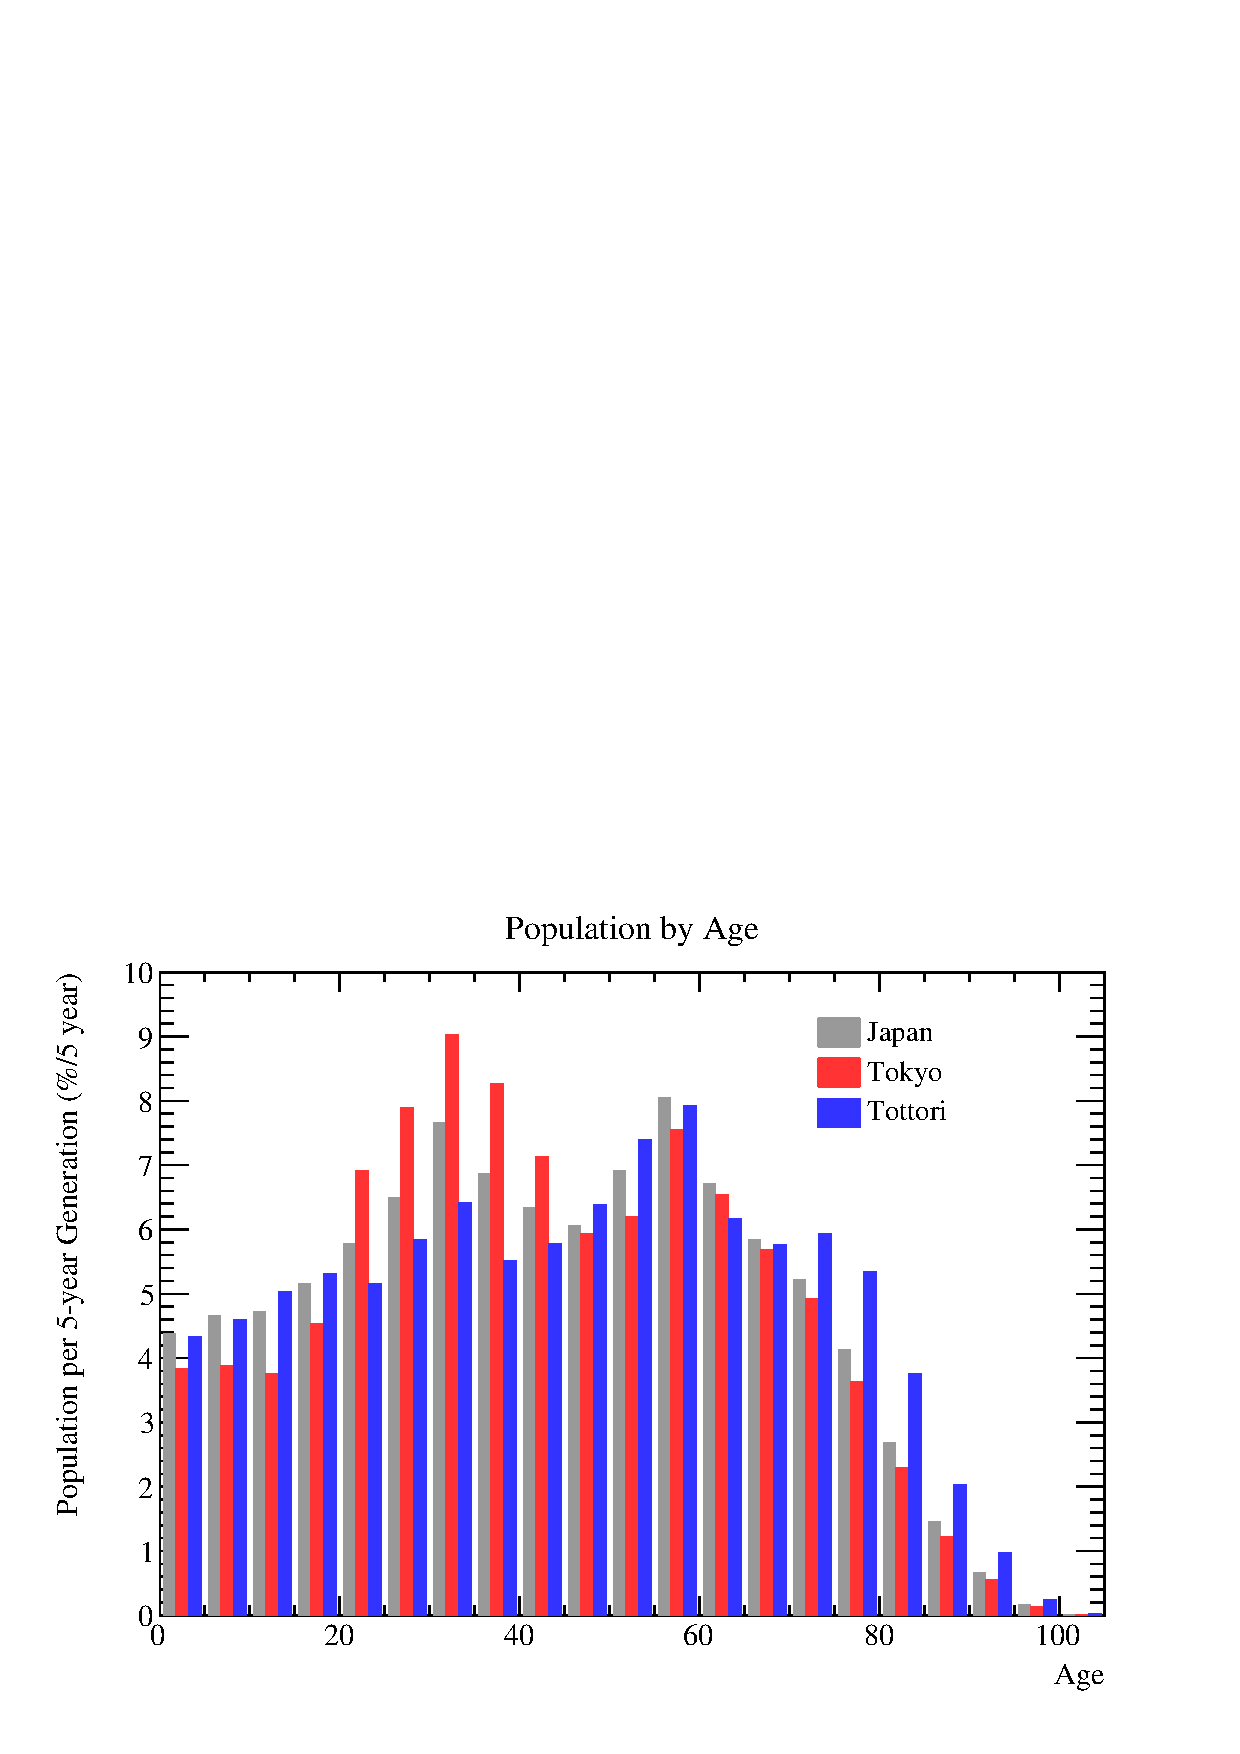
\includegraphics[width=12cm,clip]{fig/population.pdf}
  \caption{2005年国勢調査を元にした、全国合計、東京都、島根県の年齢別人口分布。コード\ref{code:frame_fill_color}で同じ結果を得られる。データは\url{http://www.e-stat.go.jp/SG1/estat/List.do?bid=000001007609&cycode=0}から入手可能。}
  \label{fig:population_pdf}
\end{figure}

ヒストグラムを使うと、その測定対象がどのような値を取りやすいのかが、一目瞭然になります。図\ref{fig:population_pdf}の元データは、総務省統計局のまとめた国勢調査の結果です。コード\ref{code:population_dat}のような、単なる数字の羅列を見ただけでは、このデータがどのような特性を持っているのかを視覚的に認識することは大変困難です。どのような年齢層に人口が偏っているのか、東京のような都市部と鳥取のような地方では、人口分布の特徴がどうなっているのか、こういう情報はヒストグラムにして比較するのが一番です。図\ref{fig:population_pdf}と図\ref{fig:population2_pdf}は、コード\ref{code:population_C}で作成しました。

%\begin{NoFloat}
\lstinputlisting[language=TeX,float=tb,caption=\texttt{population.dat},label=code:population_dat,numbers=left]{src/population.dat}
%\end{NoFloat}

ヒストグラムを「読む」上で大切な点は、棒の1本ずつの面積が意味を持つということです。図\ref{fig:population_pdf}を見ると、0〜5歳の人口は全国平均で約4.5\%になっています。ただし、縦軸の値は「\%」ではなく「\%/5 year」になっていることに注意してください。1つの棒の幅が5年間分あるので、縦軸の値に5年間をかけて、単位が「\%」になった人口の割合が出てくるわけです\footnote{新聞などで見かける図表の多くは、縦軸の単位を省略して単純に「\%」を使うことが多いですが、我々のように物理量を単位を含めて正確に扱う場面では、分母が何であるのか注意してください。}\footnote{図\ref{fig:population_pdf}では、3つのヒストグラムを並べて表示するために棒の幅を5年間よりも細くしています。5年間分の太さにするほうがより正確な表現ですが、この図では(本来の幅が常識で判断できるため)見やすさを優先してあります。}。

%\begin{NoFloat}
\lstinputlisting[language=c++,breaklines=true,caption=\texttt{population.C},label=code:population_C,numbers=left]{src/population.C}
%\end{NoFloat}

\subsection{ビン}

図\ref{fig:population_pdf}の横軸は、0〜105歳を21の区間に分けてあります。このような小分けした区間のことを、ビン(bin)と呼びます。またそれぞれのビンの幅が5歳分に相当し、これをビン幅(bin width)と呼びます。この例の21という数を、ビン数などと呼ぶことがあります。同じデータに対してビン数を変化させても、ヒストグラムの総面積は一定であることに注意してください。

\subsection{折れ線グラフとの違い}

ヒストグラムの用途は、ある測定値の範囲にどれだけの事象(イベント)が存在するかを図示することです。したがって、測定値には幅が存在し、特定の測定値で代表することはできません。先ほどの図\ref{fig:population_pdf}の例では、最初の棒は$0$〜$5$歳の人口を表していました。縦軸の値は、中心値の$2.5$歳を代表するものではないことに注意してください。

従って、図\ref{fig:population_pdf}を図\ref{fig:population2_pdf}のように折れ線グラフにして表示するのは誤りです。折れ線グラフにする場合は、1つ1つの点の座標がともに(誤差の範囲内で)意味のある1つの数値でなくてはいけません。折れ線グラフを使用するのは、原則として線分の傾きに意味がある場合に限ります。

\begin{figure}
  \centering
  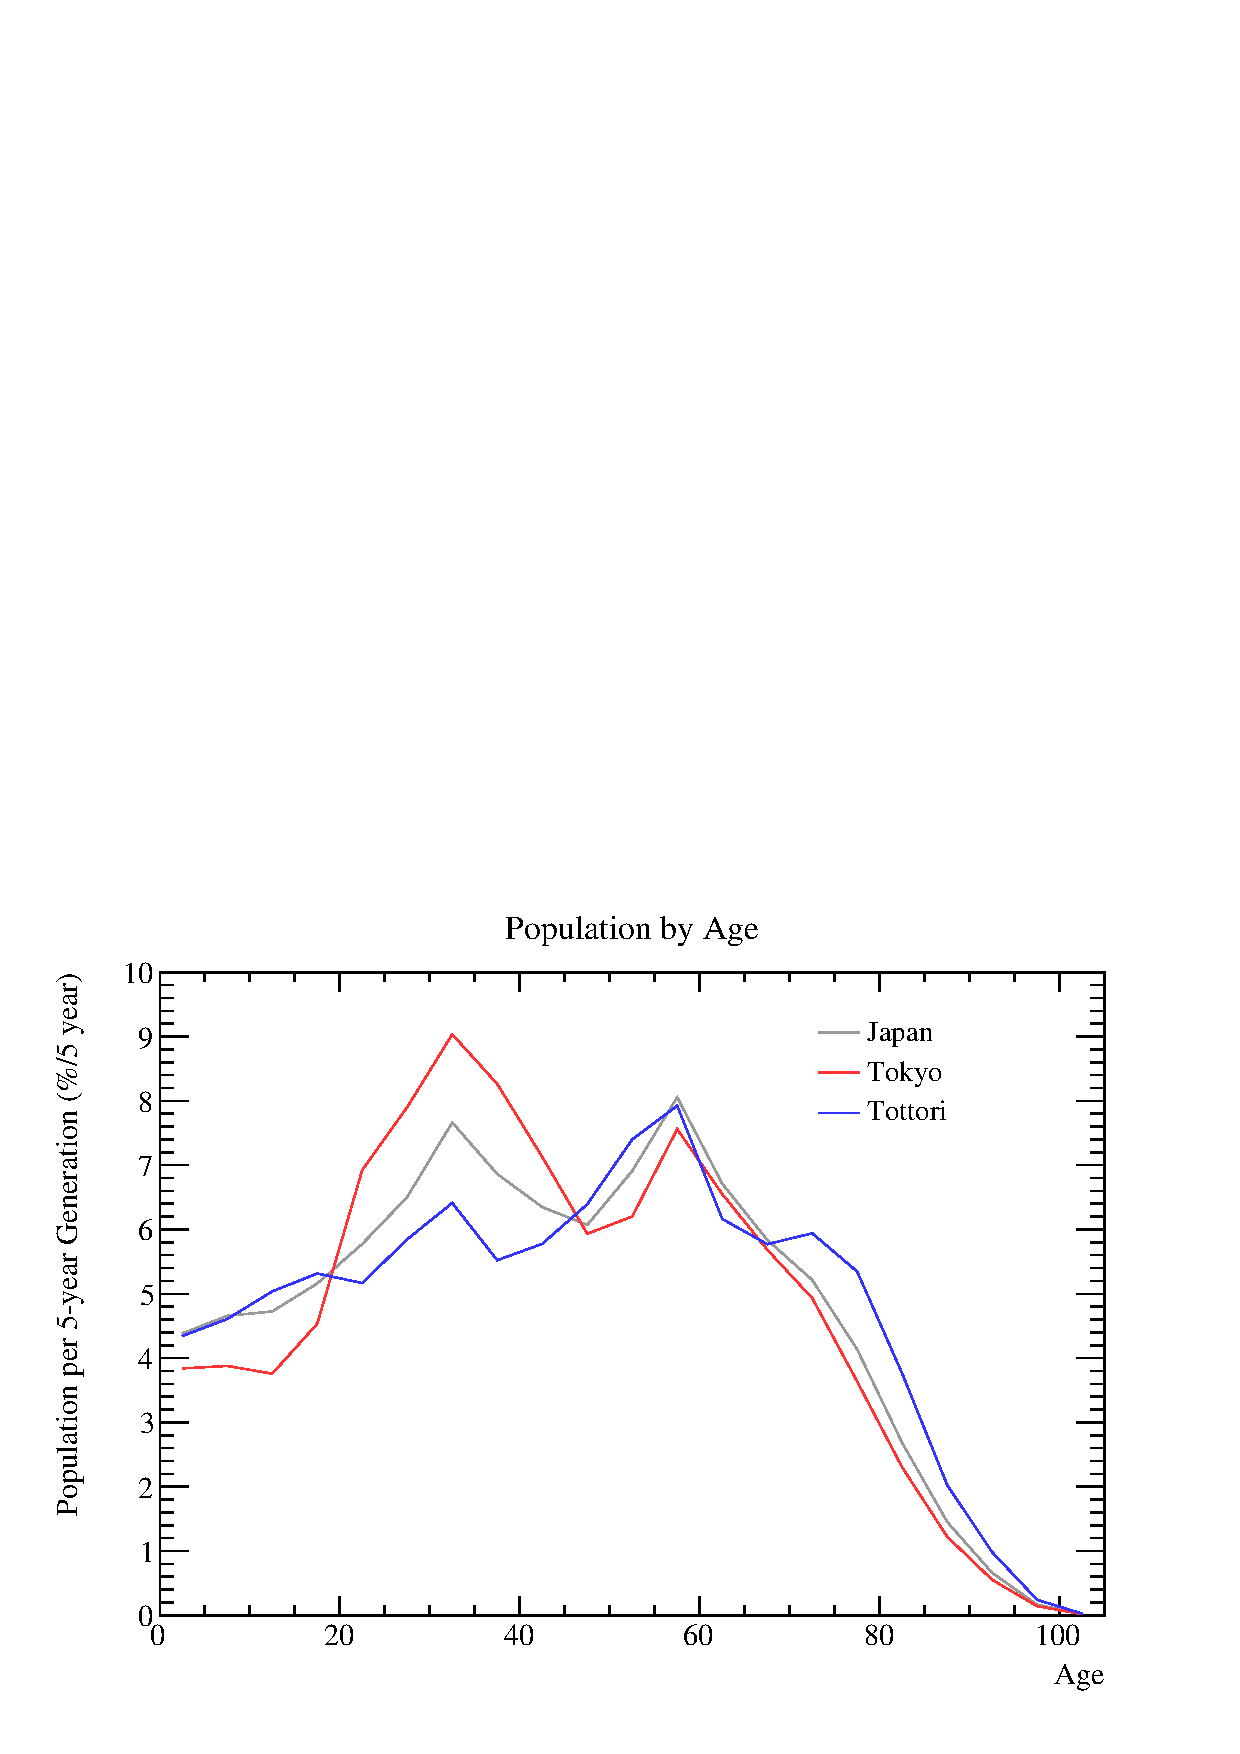
\includegraphics[width=12cm,clip]{fig/population2.pdf}
  \caption{図\ref{fig:population_pdf}の間違った表示方法の例}
  \label{fig:population2_pdf}
\end{figure}

図\ref{fig:population2_pdf}では意図的に不適切な表示をしましたが、実際に、研究者といえどもヒストグラムの間違った使い方をしている場合があります。例えば福島第一原発の事故後、東京大学柏キャンパスの柏地区環境安全管理室ではキャンパス内の 空間線量率の測定を行いました\footnote{\url{http://www.kashiwa.u-tokyo.ac.jp/kankyo/ks201111/}}。多数の測定点での空間線量率の分布として、図\ref{fig:Kashiwa_png}を掲載しています。

\begin{figure}
  \centering
  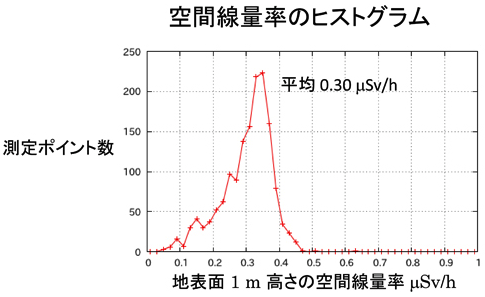
\includegraphics[scale=0.8]{fig/Kashiwa.png}
  \caption{東京大学柏キャンパス内の空間線量率の分布(柏地区環境安全管理室より引用)}
  \label{fig:Kashiwa_png}
\end{figure}

既に説明した通り、図\ref{fig:Kashiwa_png}の表示方法は不適切です。ヒストグラムは棒グラフで描くべきであり、折れ線グラフにしてはいけません。点と点を線で結んで良いのは、その傾きに意味があるときです。図\ref{fig:Kashiwa_png}の縦軸の単位は、正確に書く と「ポイント数/($0.02\ \mu\mathrm{Sv/h}$)」になります\footnote{「ポイント数」は本当は「単位」ではありません。}。しかしヒストグラムが折れ線で結ばれてしまっているため、このグラフを積分しても、実際の測定点数と同じにはならないでしょう。繰り返しますが、ヒストグラムはどのようなビン幅で作図しても面積は一定です。

\section{1次元ヒストグラム}

それでは、ROOTでどのようにヒストグラムを扱うのか順番に説明します。まずは1次元のヒストグラムからです。 ROOTには1次元のヒストグラムを扱うためのクラスが複数存在します。純粋仮想クラスである\texttt{TH1}、それを継承した\texttt{TH1C}、\texttt{TH1S}、\texttt{TH1I}、\texttt{TH1F}、\texttt{TH1D}です。最初は\texttt{TH1D}だけ覚えておけば十分です\footnote{\texttt{TH1D}は、それぞれのbinに詰まった値が\texttt{Double\_t}型で保存されます。\texttt{TH1C}、\texttt{TH1S}、\texttt{TH1I}、\texttt{TH1F}はbinの値が\texttt{Char\_t}、\texttt{Short\_t}、\texttt{Int\_t}、\texttt{Float\_t}型で保存されます。消費されるメモリの量、整数で値を保持したいかそれとも浮動小数でも良いか、などを考慮して使うヒストグラムのクラスを選択します。}。

それでは\texttt{TH1D}の簡単な使い方の説明です。まずROOTを起動し、次の操作を行って下さい。図\ref{fig:TH1D_eps}のような図が表示されるはずです。

\begin{lstlisting}[language=c++,mathescape]
root [0] TH1D* hist = new TH1D("hist", "Gaussian Distribution", 100, -10, 10)
(TH1D *) 0x7fc56c639860
root [1] hist->GetXaxis()->SetTitle("Physics Quantity #it{X}")
root [2] hist->GetYaxis()->SetTitle("Entries")
root [3] const Double_t kMean = 3.
(const Double_t) 3.00000
root [4] const Double_t kSigma = 2.
(const Double_t) 2.00000
root [5] for(Int_t i = 0; i < 10000; i++){
root ($\conted$, cancel with .@) [6] Double_t x = gRandom->Gaus(kMean, kSigma);
root ($\conted$, cancel with .@) [7] hist->Fill(x);
root ($\conted$, cancel with .@) [8] }
root [9] hist->Draw()
Info in <TCanvas::MakeDefCanvas>:  created default TCanvas with name c1
root [10] hist->GetMean()
(Double_t) 3.00946
root [11] hist->GetMeanError()
(Double_t) 0.0198828
root [12] hist->GetStdDev()
(Double_t) 1.98778
root [13] hist->GetStdDevError()
(Double_t) 0.0140593
\end{lstlisting}

\begin{figure}
  \centering
  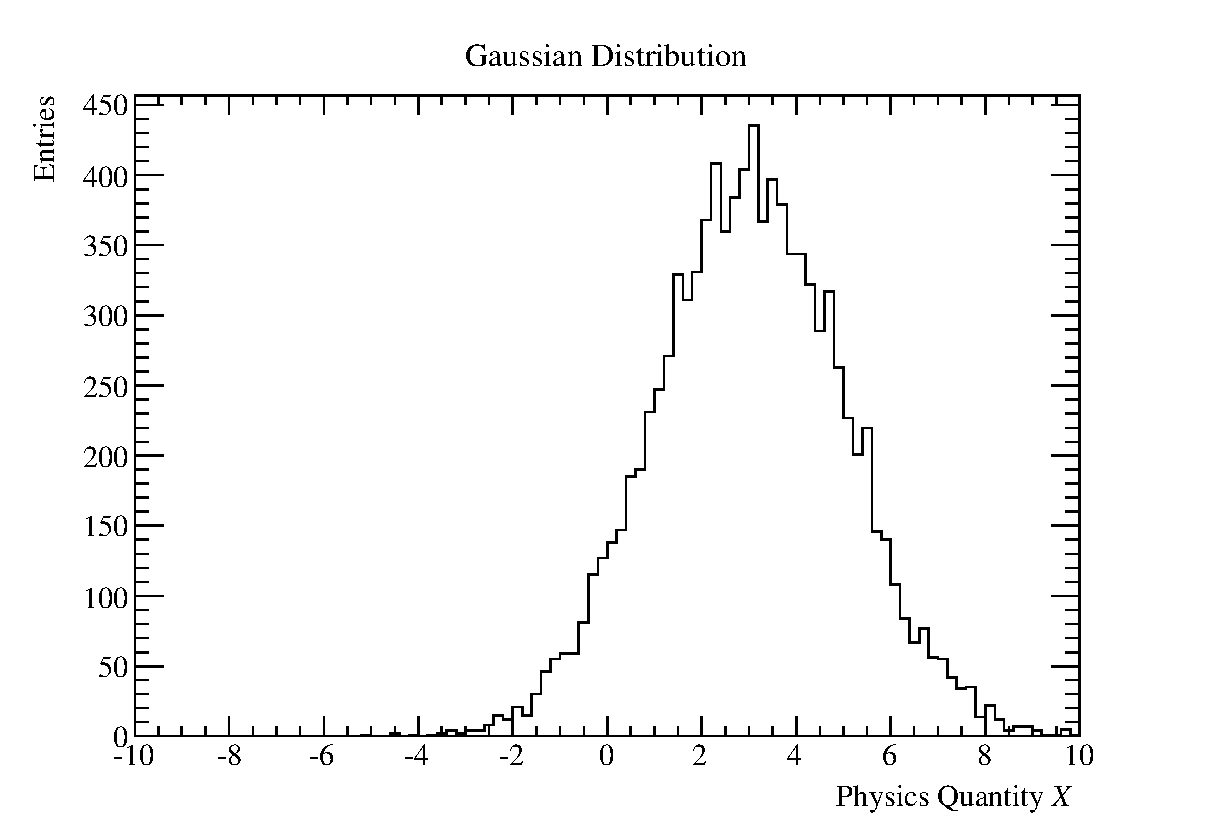
\includegraphics[width=12cm,clip]{fig/TH1D.eps}
  \caption{物理量$X$(平均$\mu = 3$、標準偏差$\sigma = 2$)のガウス分布の例}
  \label{fig:TH1D_eps}
\end{figure}

\section{2次元ヒストグラム}

\begin{lstlisting}[language=c++,breaklines=true,mathescape]
root [0] TH2D* h2 = new TH2D("h2", "2D Gaussian Distribution;#it{x};#it{y};Entries", 100, -10, 10, 100, -10, 10)
(TH2D *) 0x7fe8c3615eb0
root [1] const Double_t kSigma = 2.
(const Double_t) 2.00000
root [2] for(Int_t i = 0; i < 100000; i++){
root ($\conted$, cancel with .@) [3] Double_t x = gRandom->Gaus(0, kSigma);
root ($\conted$, cancel with .@) [4] Double_t y = gRandom->Gaus(0, kSigma);
root ($\conted$, cancel with .@) [5] h2->Fill(x, y);
root ($\conted$, cancel with .@) [6] }
root [7] TCanvas* can = new TCanvas("can", "can", 600, 600)
(TCanvas *) 0x7fe8c359a9a0
root [8] h2->Draw("colz")
\end{lstlisting}

\begin{figure}
  \centering
  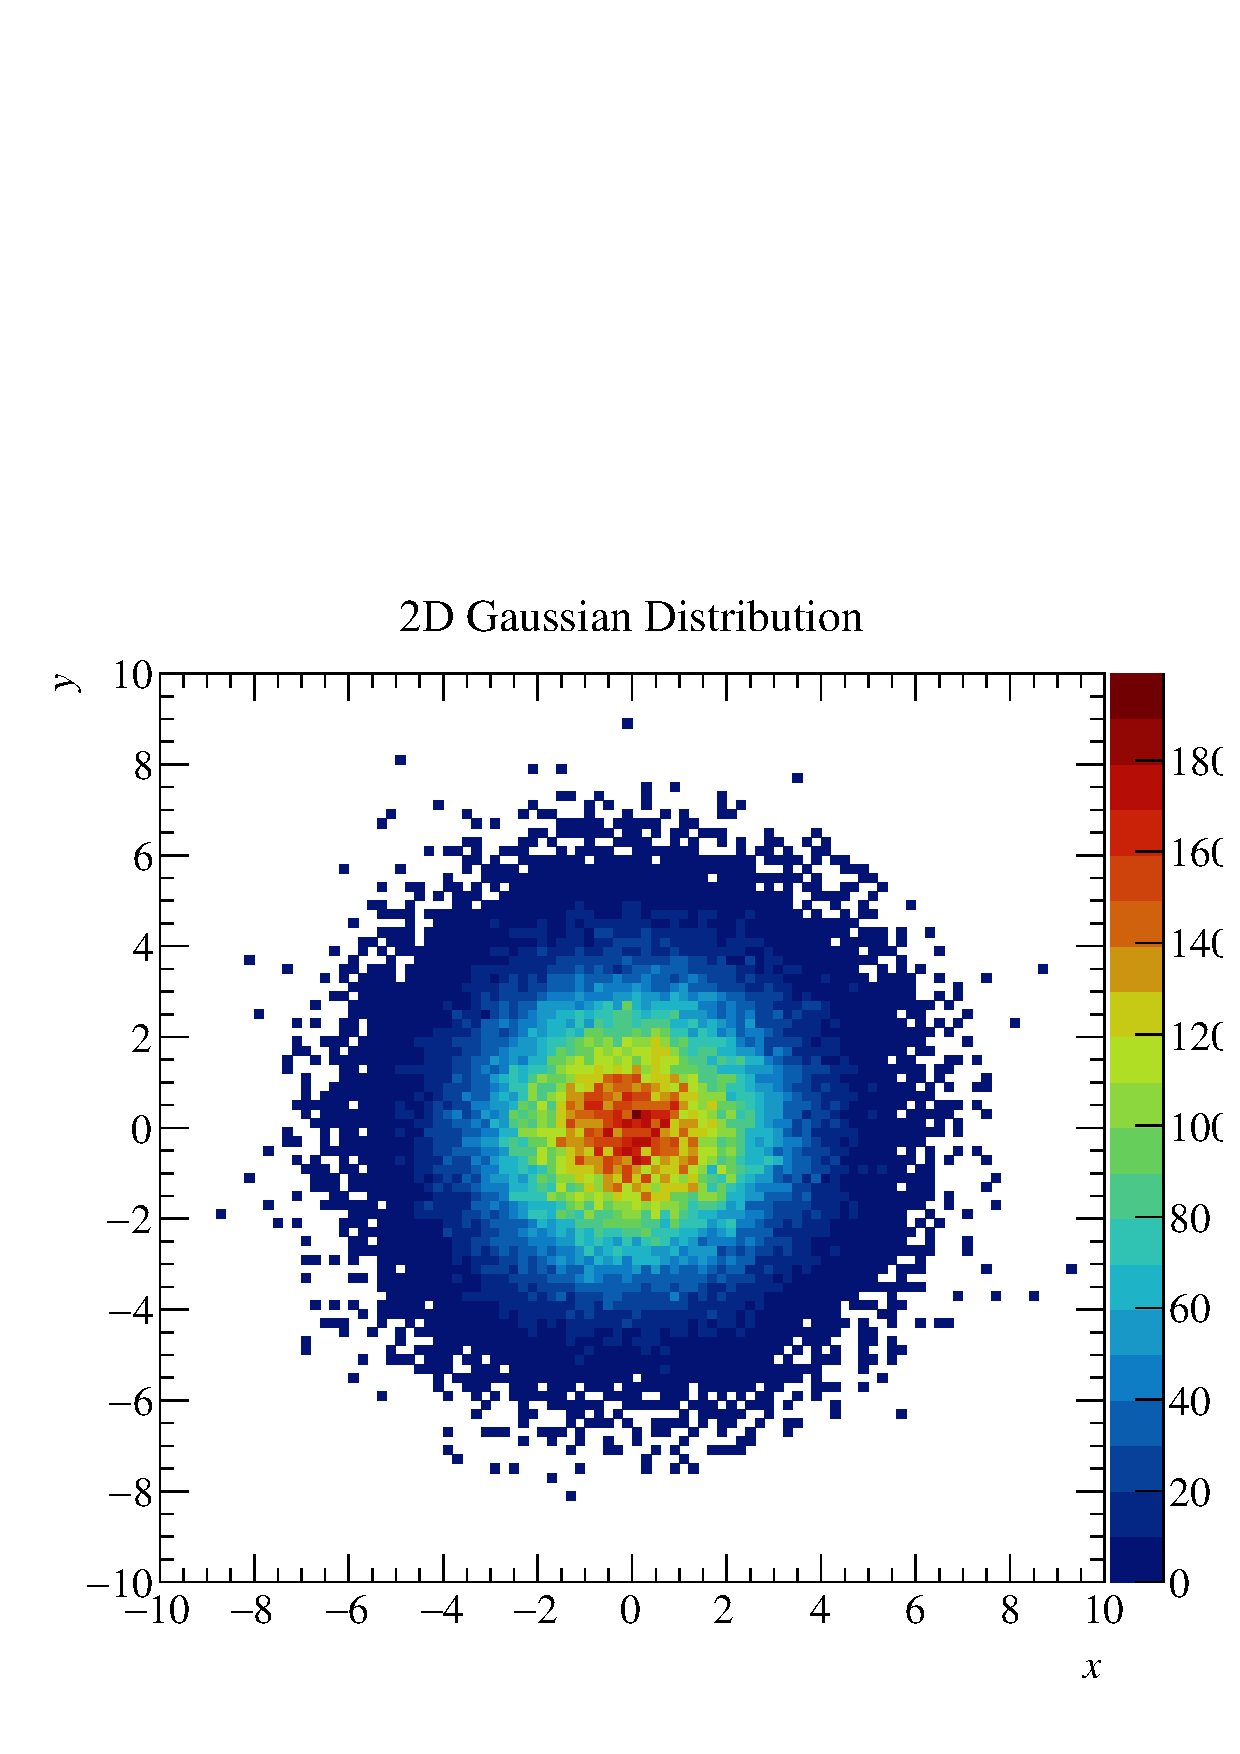
\includegraphics[width=12cm]{fig/TH2D.pdf}
  \caption{物理量$x$、$y$(平均$\mu_x = \mu_y = 0$、標準偏差$\sigma = 2$)の 2 次元ガウス分布の例}
  \label{fig:TH2D_pdf}
\end{figure}

\section{3次元ヒストグラム}

\chapter{グラフ}
\chapter{Tree}
\chapter{Python}
\label{chap:Python}

\section{注意}
Python に関係する技術の発展は ROOT のそれより目覚ましく、この文書も含め、ウェブ上に転がる情報が簡単に陳腐化します。これはオープンソースコミュニティの活発さや、Python という言語の人気のためです。ここに書かれている情報は 2020 年 4 月現在、筆者の知る限りの範囲で、なるべく新しいものになるように務めていますが、数年で古くなるということを知っておいてください。またPython環境の構築は様々なやり方があり、どれも一長一短で、本書で網羅するのは困難です。そのため、本書では筆者が初心者向けに個人的に推奨する方法のみを解説します。

Python環境をCondaを使って構築する場合は、HomebrewやYumを使ってPythonをインストールする必要はありません。またCondaでインストール可能なPythonパッケージは、基本的に\texttt{pip}でインストールする必要はないと思うので、適宜読み飛ばすなり、Condaに読み替えてください。

\section{なぜPythonを使うのか}

Pythonとはプログラミング言語の1つです。第\ref{chap:C++}章で説明した概念は、ほぼそのままPythonでも通用します。C++と異なる点は、例えば以下のようなものが挙げられます。
\begin{itemize}
  \item コンパイルしなくてもコードを実行可能な、スクリプト言語と呼ばれるものです。これはROOTのClingに似ています。
  \item 様々なパッケージが標準で用意されており、C++に比べると、手軽に様々な機能を使うことができます。例えば、オプション解析の機能が標準で利用可能です。
  \item 物理、天文業界でPythonを利用する研究者が近年増えており、データ解析に必要な外部パッケージが多く用意されています。
  \item Linux/Mac/WindowsといったOS環境を気にせずに使うことができます。
\end{itemize}
特に3つ目は重要で、ROOT、IRAF、DS9、Geant4、FITSといったものを、Pythonという1つの言語の中で同時に扱えるようになります。もちろん、これらの機能をC++から呼び出してコンパイルすることも可能です。しかし、リンクすべきライブラリやヘッダーファイルを把握し、どのような環境でも確実に動作するプログラムを組むのは大変なことです。Pythonであれば、OSを意識せずに様々な機能を簡単に使うことができます。

例えば、エネルギー、座標、時間などで構成される光子イベントがFITSのバイナリテーブルで用意されているとしましょう。このイベントのエネルギー分布をROOTのヒストグラムに詰めたいと思った場合、以下のような簡単なコードで作業が終了します。もしあなたがこのコードを見て、短くて簡単だと感じるならば、ぜひPythonに挑戦してみましょう。

\begin{lstlisting}[language=python]
In [1]: import ROOT
In [2]: from astropy.io import fits 
In [3]: hist = ROOT.TH1D("hist", "Energy distribution;Energy (MeV)", 100, 0, 1e3
   ...: )
In [4]: energies = fits.open("photon/lat_photon_weekly_w009_p302_v001.fits")[1]
   ...: .data.field("ENERGY")
In [5]: for i in range(energies.size):
   ...:     hist.Fill(energies[i])
In [6]: hist.Draw()
Info in <TCanvas::MakeDefCanvas>:  created default TCanvas with name c1
\end{lstlisting}

\section{簡単に使ってみる}
Python は ROOT と同様にコマンドラインからインタープリタを呼び出して 1 行ずつコマンドを実行することもできれば、スクリプトにまとめて実行することもできます。

\subsection{起動と終了}
まず Python(ここでは IPython)のインタープリタに 1 行ずつ命令を渡していく操作を試してみましょう。面白い例ではありませんが、\ref{sec:helloworld}~節で解説したC++の \texttt{hello\_world.cxx} を Python に直してみましょう。

まず IPython を起動します。IPythonが入っていない場合、まずは\ref{sec:Python_Install}~節と\ref{sec:IPython}~節を読んでIPythonをインストールしてください。

\begin{lstlisting}[language=bash]
$ ipython
Python 3.7.7 (default, Mar 10 2020, 15:43:33) 
Type 'copyright', 'credits' or 'license' for more information
IPython 7.13.0 -- An enhanced Interactive Python. Type '?' for help.

In [1]: 
\end{lstlisting}

次に、C の \texttt{printf} に似た関数である \texttt{print} 関数を使って、「Hello World!」という文字列を出力してみます。
\begin{lstlisting}[language=python]
In [1]: print('Hello World!')
Hello World!
\end{lstlisting}

Python 2 までは \texttt{print} 関数の使い方として、次のような例がよく用いられていました。しかし Python 3 では多くの仕様が変更になり、このような \texttt{print} 関数の使い方は Python~3 で動作しなくなりました。書籍やインターネット上にある情報は Python~2 と Python~3 のものが混在していますので、注意してください。

\begin{lstlisting}[language=python]
In [1]: print 'Hello World!'
Hello World!
\end{lstlisting}

最後に、Ctrl-D を入力すると IPython を終了できます\footnote{Control キーを押しながら、D キーを同時に押す}。本当に終了して良いのか聞かれるので、良い場合はそのまま Enter キーを、IPython を続ける場合は N キーを押してから Enter キーを押します。

\begin{lstlisting}[language=python]
In [2]:
Do you really want to exit ([y]/n)? 
$ 
\end{lstlisting}

\subsection{スクリプトの書き方}

Python スクリプトの使い方は、大別して三通りあります。

\section{Python~3のインストール}
\label{sec:Python_Install}

macOSやCentOS~7では、標準でPythonがインストールされているはずです。ただし、このPythonのバージョンはPython~2のため、特にこだわりが無くPythonをこれから新たに習得する人は、Python~3を導入して使い始めることを推奨します。

\subsection{macOS Mojave の場合}

macOS で新たにソフトウェアを追加する場合、節~\ref{sec:Homebrew}で説明する通り、Homebrewというパッケージ管理システムを使うのが一般的です。ここではHomebrewがすでに入っているという前提で説明します。

次のコマンドを実行することで、\texttt{python3}、\texttt{pip3}、\texttt{ipython}などがインストールされます。
\begin{lstlisting}[language=bash]
$ brew install ipython
\end{lstlisting}
Homebrewでは\texttt{ipython}は\texttt{python}に依存しているため、macOS標準のPythonとは別のPythonをHomebrewが自動でインストールします。特に指定をしない場合、このPythonはPython~3になります。

問題なく Python~3 が入ったことを確かめるため、\texttt{python3}コマンドを実行してみます。次のように表示されれば成功です。
\begin{lstlisting}[language=bash]
ult, Mar 10 2020, 15:43:03) 
[Clang 11.0.0 (clang-1100.0.33.17)] on darwin
Type "help", "copyright", "credits" or "license" for more information.
>>> 
\end{lstlisting}
IPythonも確認してみましょう。
\begin{lstlisting}[language=bash]
$ ipython3
Python 3.7.7 (default, Mar 10 2020, 15:43:03)
Type 'copyright', 'credits' or 'license' for more information
IPython 7.13.0 -- An enhanced Interactive Python. Type '?' for help.

In [1]:
\end{lstlisting}

Mojave上のHomebrewではPython~3のコマンドを\texttt{python3}や\texttt{python3.7}としてインストールし、\texttt{python}コマンドはデフォルトの\texttt{/usr/bin/python}としてPython~2のまま残ります。ただし、他の環境では\texttt{python2}がPython~2で\texttt{python}がPython~3だったりするので、自分がPython~2を使っているのかPython~3を使っているのか、よく注意してください。

\begin{lstlisting}[language=bash]
$ python
Python 2.7.10 (default, Feb 22 2019, 21:17:52) 
[GCC 4.2.1 Compatible Apple LLVM 10.0.1 (clang-1001.0.37.14)] on darwin
Type "help", "copyright", "credits" or "license" for more information.
>>> 
\end{lstlisting}

\subsection{macOS Catalina の場合}
macOS Catalinaでは、標準でPython~3が\texttt{/usr/bin/python3}に入っています。しかしIPythonが入っていないので、Mojaveと同様の方法で、HomebrewでIPythonとともにインストールしてください。

この場合HomebrewでインストールするPython~3は\texttt{/usr/local/bin/python3}になります。
\begin{lstlisting}[language=bash]
$ which python3
/usr/local/bin/python3
$ /usr/local/bin/python3 --version
Python 3.7.7
$ /usr/bin/python3 --version 
Python 3.7.3
\end{lstlisting}

\subsection{CentOS~7 の場合}

CentOS~7のようなRed Hat Enterprise Linux(RHEL)クローンと呼ばれるLinuxディストリビューションでは、\texttt{yum}(ヤム)と呼ばれるパッケージ管理システムが標準的に使われます。多くのソフトウェアを\texttt{yum}から入手可能ですが、Python~3 は標準では入れられないため、まずレポジトリを追加します。

\begin{lstlisting}[language=bash]
$ sudo yum install -y https://centos7.iuscommunity.org/ius-release.rpm
\end{lstlisting}

これで\texttt{yum}がソフトウェアを検索する際の新たな場所が追加されます。次に\texttt{python36u-devel}をインストールし、\texttt{python3.6}と\texttt{pip3.6}をインストールします。

\begin{lstlisting}[language=bash]
$ sudo yum install python36u-devel
$ sudo yum install python36u-pip
\end{lstlisting}

これで、\texttt{python3.6}を実行するとPython~3.6を起動することができるようになりました。
\begin{lstlisting}[language=bash]
$ which python3.6
/usr/bin/python3.6
$ python3.6
Python 3.6.7 (default, Dec  5 2018, 15:02:05) 
[GCC 4.8.5 20150623 (Red Hat 4.8.5-36)] on linux
Type "help", "copyright", "credits" or "license" for more information.
>>> 
\end{lstlisting}

デフォルトで入っているPythonは2.7.5です。これは\texttt{/usr/bin/python}として残ります。
\begin{lstlisting}[language=bash]
$ which python
/usr/bin/python
$ python
Python 2.7.5 (default, Aug  4 2017, 00:39:18) 
[GCC 4.8.5 20150623 (Red Hat 4.8.5-16)] on linux2
Type "help", "copyright", "credits" or "license" for more information.
>>> 
\end{lstlisting}

次に\texttt{pip3.6}を使ってPython~3用のIPythonをインストールします。

\begin{lstlisting}[language=bash]
$ which pip3.6 
/usr/bin/pip3.6
$ sudo pip3.6 install ipython
$ sudo pip3.6 install --upgrade pip
\end{lstlisting}

Python~2用のIPythonを入れていない場合、\texttt{/usr/bin/ipython}と\texttt{/usr/bin/ipython3}がPython~3用のIPythonになります。

\begin{lstlisting}[language=bash]
$ which ipython
/usr/bin/ipython
$ which ipython3
/usr/bin/ipython3
$ ipython3 
Python 3.6.7 (default, Dec  5 2018, 15:02:05) 
Type 'copyright', 'credits' or 'license' for more information
IPython 7.4.0 -- An enhanced Interactive Python. Type '?' for help.

In [1]:
\end{lstlisting}

\section{\texttt{pip}}

すでに前節までで見たように、\texttt{pip}もしくは\texttt{pip3}というコマンドを使ってPythonの追加パッケージをインストールする方法を説明しました。この\texttt{pip}(ピップ)というコマンドはPythonのコミュニティで広く使われているパッケージ管理システムのひとつです。Python Package Index(PyPI、パイピーアイ)\footnote{\url{https://pypi.org}}に登録されている様々な追加パッケージを自動でインストールします。通常は \texttt{/usr/local/lib/python/site-package} という場所に新しいパッケージが追加されます。

\texttt{pip} の基本は次のコマンドです。\texttt{search}でその名前のパッケージの情報やすでにインストールされているかを調べ、\texttt{install}でインストールします。Python~3の場合は\texttt{pip3}と読み替えてください。
\begin{lstlisting}[language=bash]
$ pip search PACKAGE_NAME
$ pip install PACKAGE_NAME
\end{lstlisting}  

\section{IPython}
\label{sec:IPython}
IPython

\section{Pythonの基本}

\section{PyROOT}

\subsection{C++からPythonへ}

\subsection{メモリ管理}

\section{PyFITS}

\chapter{様々な技}

ROOTでそこそこ格好良い図を作るには、ある程度の知識と慣れが必要になります。ここでは、いくつかのスクリプトとその出力結果を例示し、ROOTで望み通りの図を作るにはどうすれば良いかを紹介します。

\section{色関連}
\subsection{自前のカラーパレットを定義する}

ROOTでは、2次元ヒストグラムや2次元グラフの「高さ」を表現する手段として、色を用いることができます。これは第\ref{chap_Histogram}章でも説明しました。ROOTはいくつかのカラーパレット(color palette)を用意してくれていますが、それらの実用性は乏しいと言わざるを得ません。例えば図\ref{fig_multi_palette_pdf}の左上に示したような、デフォルトのカラーパレットを使っている人はほとんど見かけません。また階調数が小さめに設定されているため、滑らかな色表現には向きません。唯一よく使われているのが、以下の設定です。
\begin{lstlisting}[language=C++]
root [0] gStyle->SetPalette(1)
\end{lstlisting}
レインボーカラー(rainbow color)などと呼ばれることがあります。他にデフォルトで用意されているパレットについては、\url{http://root.cern.ch/root/html/TColor.html#TColor:SetPalette}を参照してください。

コード\ref{code_color_def}では、自分好みのカラーパレットを作る方法を示しています。原理は単純で、作りたいパレットに応じて、\texttt{TColor::CreateGradientColorTable}を呼び出すための関数を用意するだけです。いくつか例を書きましたが、原理は一緒なので関数BPalette()の解説のみをします。

\begin{NoFloat}
\lstinputlisting[language=c++,caption=\texttt{color\_def.C},label=code_color_def,numbers=left]{src/color_def.C}
\end{NoFloat}

次の4行が、実際に色の設定をする部分です。
\begin{lstlisting}[language=c++]
  Double_t r[] = {0., 0.0, 1.0, 1.0, 1.0}; 
  Double_t g[] = {0., 0.0, 0.0, 1.0, 1.0}; 
  Double_t b[] = {0., 1.0, 0.0, 0.0, 1.0}; 
  Double_t stop[] = {0., .25, .50, .75, 1.0}; 
\end{lstlisting}
最初の3行でRGB各色の輝度情報を設定します。例えば$\mathrm{R}=\mathrm{G}=\mathrm{B}=1$であれば白、$\mathrm{R}=\mathrm{G}=\mathrm{B}=0$であれば黒、$\mathrm{R}=\mathrm{G}=1$、$\mathrm{B}=0$であれば黄色といった具合です。次の行は、それらの色がヒストグラムの最小値($\equiv0$)から最大値($\equiv1$)のどこに相当するかを決めています。

グラデーションをROOTに登録する作業は、
\begin{lstlisting}[language=c++]
  Int_t index = TColor::CreateGradientColorTable(5, stop, r, g, b, kN);
\end{lstlisting}
で行います。最後の引数は、階調の数です。これを大きくすればより滑らかなグラデーションになります。これらの関数が複数回呼び出されても速度低下を招かないように、関数内静的変数を用いていることに注意してください。

ガンマ線のカウントマップでは、よくこの\texttt{BPalette()}が使われます\footnote{\texttt{BPalette}という名前は、DS9のパレットの名前に基づいています。}(図\ref{fig_multi_palette_pdf}下段)。明るいところを強調し、暗いノイジーな箇所を目立たなくするためでしょう\footnote{カラーパレットの使い方で、(良い意味でも悪い意味でも)図の印象ががらりと変わるということを心に留めておいてください。}。\texttt{GrayPalette()}と\texttt{GrayInvPalette()}は、それぞれ黒から白、白から黒へのグラデーションです(図\ref{fig_multi_palette_pdf}中段)。\texttt{RBPalette()}は、青、白、赤と変化するグラデーションです。世の中であまり使われていませんが、2次元ヒストグラムの残差を見せるときなどに筆者は使っています。

実際に作成するスクリプトでこのようなパレットを設定するためには、どこかでこれらの関数を定義しておいて、ヒストグラムを描く前に呼び出して下さい。例えば
\begin{lstlisting}[language=C++]
root [0] .L color_def.C
root [1] BPalette()
\end{lstlisting}
などとすれば良いでしょう。\texttt{\~{}/.rootlogon.C}に
\begin{lstlisting}[language=C++]
gROOT->LoadMacro("color_def.C");
\end{lstlisting}
という1行を加えて、起動時に読み込ませておくのでも大丈夫です。

\subsection{複数のカラーパレットを同時に使う}

自分の好きなようにカラーパレットを作成しても、複数のカラーパレットを同時に使うためには小技が必要です。例えば以下を実行した後に、\texttt{can1}をクリックしてみてください。
\begin{lstlisting}[language=C++]
root [0] TH2D* h2 = new TH2D("h2", "", 3, -1, 1, 3, -1, 1)
root [1] h2->Fill(0, 0)
root [2] TCanvas* can1 = new TCanvas("can1", "can1")
root [3] gStyle->SetPalette(1)
root [4] h2->Draw("colz")
root [5] TCanvas* can2 = new TCanvas("can2", "can2")
root [6] BPalette()
root [7] h2->Draw("colz")
\end{lstlisting}
クリックする直前まではレインボーパレットだったのに、クリックすると\texttt{BPalette()}の設定に変わってしまうはずです。これは、ROOTがクリックを検知した後に再描画を開始するためですが、その時点でグローバルに持っているパレットの情報が\texttt{BPalette()}に書き換えられてしまっているからです。これを回避するのが、コード\ref{code_multi_palette}です。\texttt{TExec}を「重ね塗り」することによって、再描画の直前にパレットの設定を強制的に実行することができます。

\begin{NoFloat}
\lstinputlisting[language=c++,caption=\texttt{multi\_palette.C},label=code_multi_palette,numbers=left]{src/multi_palette.C}
\end{NoFloat}

\begin{figure}
  \centering
  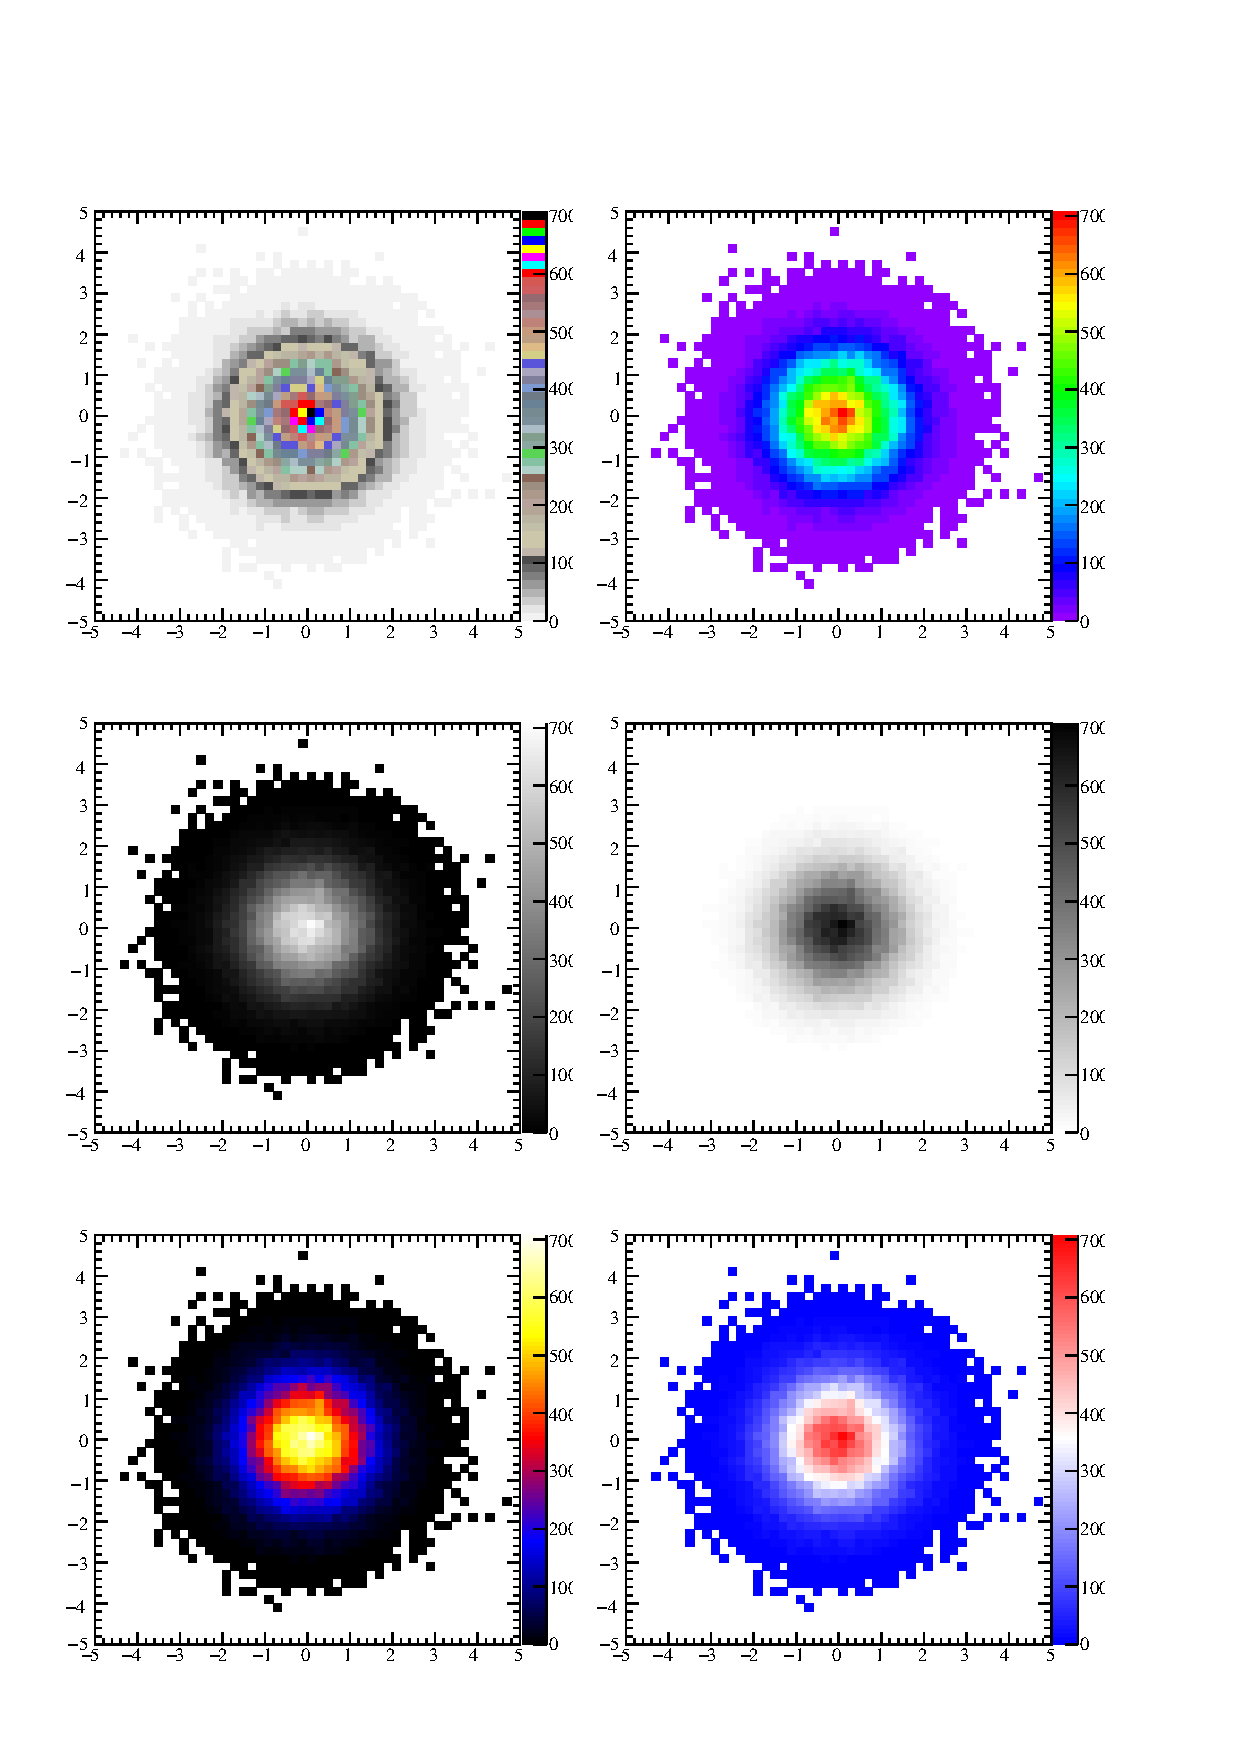
\includegraphics[width=12cm,clip]{fig/multi_palette.pdf}
  \caption{コード\ref{code_multi_palette}の出力結果}
  \label{fig_multi_palette_pdf}
\end{figure}

\subsection{塗りつぶしの色を変更する}

図\ref{fig_multi_palette_pdf}で様々なパレットを例示しました。既にお気付きの通り、値が0のビンはROOTは塗りつぶしません。そのため、空っぽのビンは全て白くなっています。図\ref{fig_multi_palette_pdf}の右上のように、パレットに白が含まれていない場合は、白いままのほうがヒストグラムの状態を把握するのに便利です。しかしパレット中に白が含まれている場合は、値が0なのか、他の値なのか判断できない場合が出てきます。そのような場合は、フレームの色を変更しましょう。

\begin{NoFloat}
\lstinputlisting[language=c++,caption=\texttt{frame\_fill\_color.C},label=code_frame_fill_color,numbers=left]{src/frame_fill_color.C}
\end{NoFloat}

コード\ref{code_frame_fill_color}は、フレームの背景色を変更する方法です。出力結果は図\ref{fig_frame_fill_color_pdf}に示します。

\begin{lstlisting}[language=C++]
  TPaletteAxis* palette 
    = (TPaletteAxis*)hist->GetListOfFunctions()->FindObject("palette"); 
\end{lstlisting}
この部分では、ヒストグラムから\texttt{TPaletteAxis}\footnote{図\ref{fig_frame_fill_color_pdf}の右端にあるグラデーション付き目盛りのことです。}のポインタを取得します。その直前の行で\texttt{gPad}を更新しないと\texttt{0}を返すので注意してください。
\begin{lstlisting}[language=C++]
  gPad->SetFrameFillColor(col); 
\end{lstlisting}
で、\texttt{gPad}の塗りつぶしの色を決定しています。この例では、最小値の色は黒になっています。

\begin{figure}
  \centering
  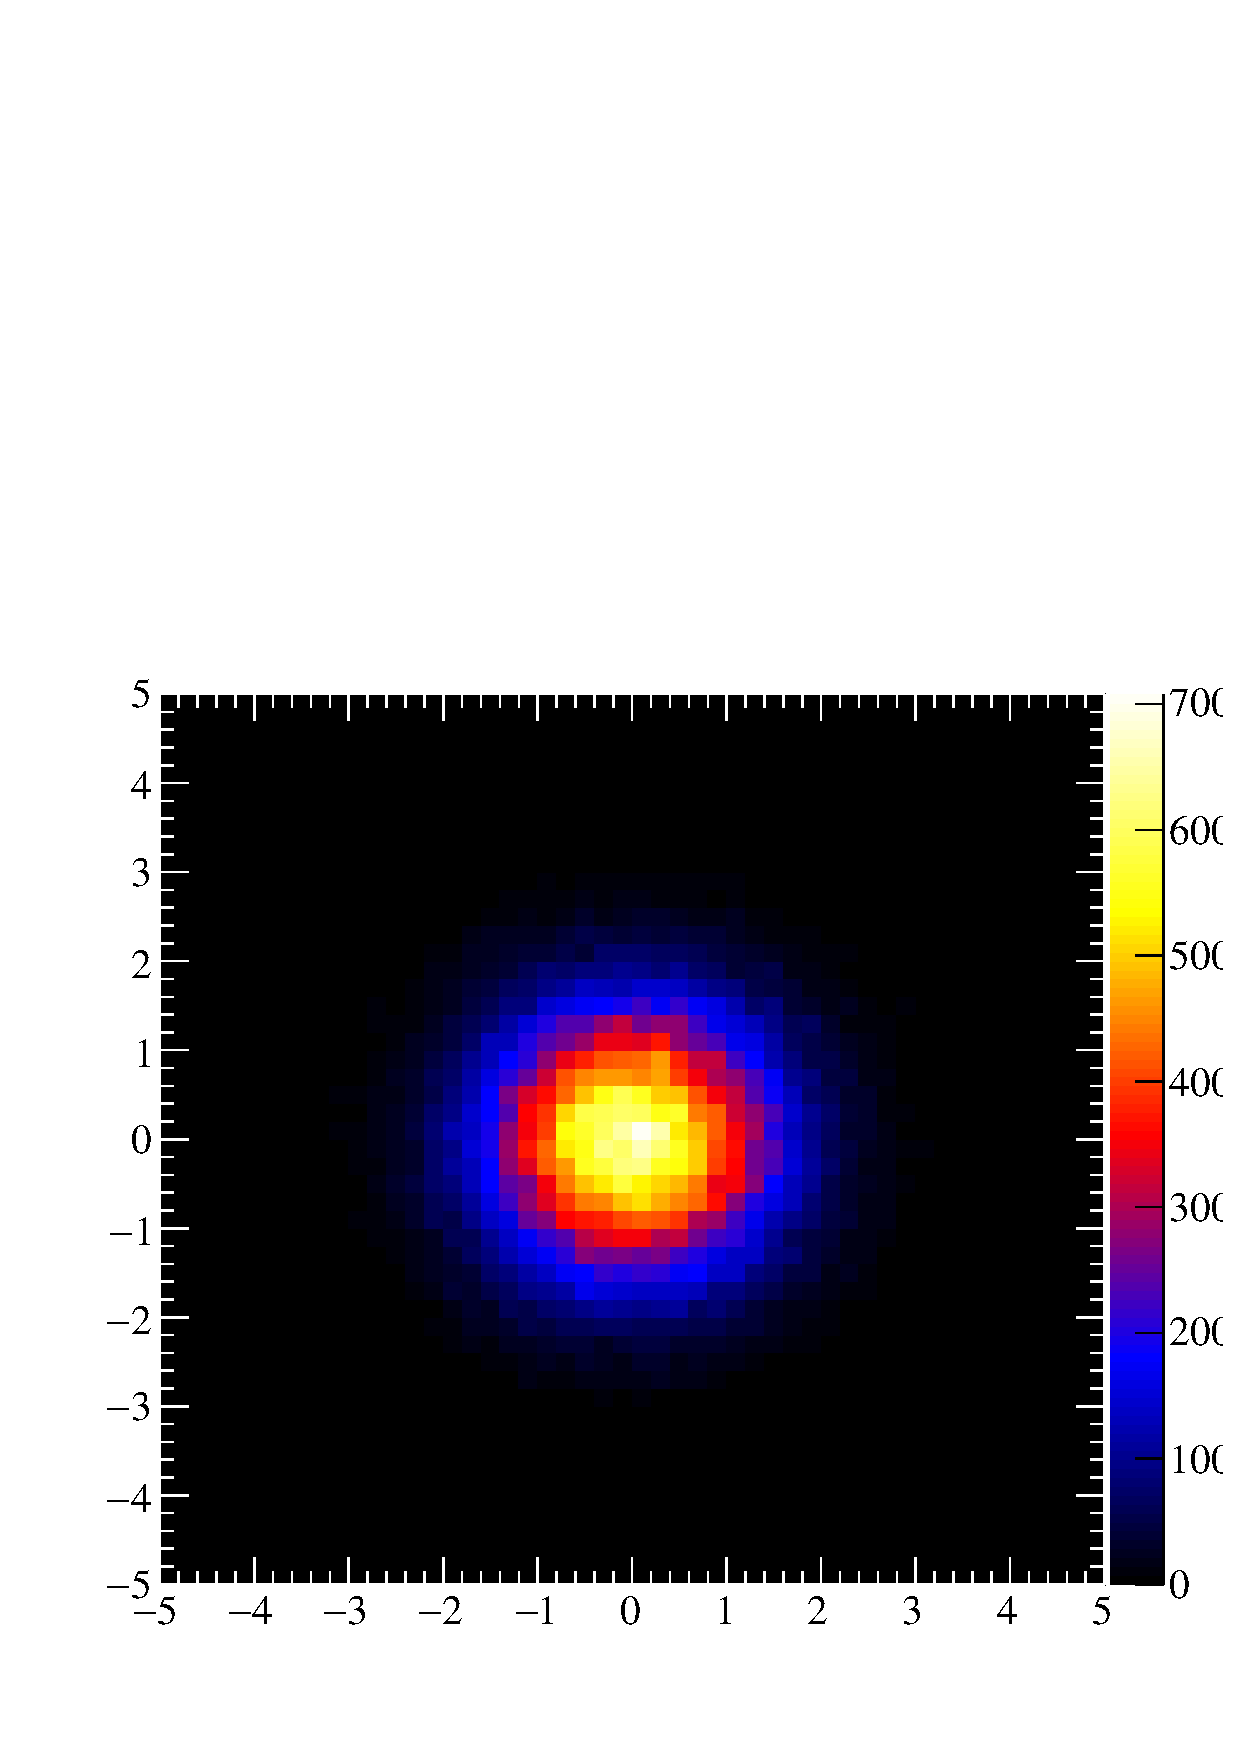
\includegraphics[width=8cm]{fig/frame_fill_color.pdf}
  \caption{コード\ref{code_frame_fill_color}の出力結果}
  \label{fig_frame_fill_color_pdf}
\end{figure}


\section{キャンバス関連}
\subsection{描画領域の大きさを指定する}
通常、新たなキャンバスを作成するときに大きさを指定する場合は、
\begin{lstlisting}[language=C++]
root [0] TCanvas* can = new TCanvas("can", "can", 100, 100)
\end{lstlisting}
のように第3、第4引数に横幅と高さを指定します。しかし予想外にも、図\ref{fig_100x100_png}に示すように、実はこの大きさは描画領域の大きさではありません。メニューバーは描画領域外周部まで含めた大きさなのです。したがって、実際に描画できる部分の大きさは、筆者の環境では$96\times72$ピクセルになってしまいます。図\ref{fig_100x100_v2_png}のように、描画領域を正確に$100\times100$ピクセルにしたい場合は、コード\ref{code_PreciseSizeCanvas}のような関数を用意しましょう。

\begin{figure}
  \centering
  \subfloat[$96\times72$ピクセル]{
    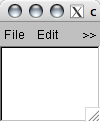
\includegraphics[width=3cm]{fig/100x100.png}
    \label{fig_100x100_png}
  }
  \hfil
  \subfloat[$100\times100$ピクセル]{
    
\includegraphics[width=3cm]{fig/100x100_v2.png}
    \label{fig_100x100_v2_png}
  }
  \caption{\texttt{TCanvas}の描画領域の違い}
\end{figure}

\begin{NoFloat}
\lstinputlisting[language=c++,caption=\texttt{PreciseSizeCanvas.C},label=code_PreciseSizeCanvas,numbers=left]{src/PreciseSizeCanvas.C}
\end{NoFloat}

次のように、\texttt{PresiceSizeCanvas.C}をロードしてから、\texttt{PresiceSizeCanvas}関数を\texttt{TCanvas}のコンストラクタのように使用すれば、描画領域が丁度$400\times400$ピクセルのキャンバスが得られます。
\begin{lstlisting}[language=C++]
root [0] .L PresiceSizeCanvas.C
root [1] TCanvas* can = new PresiceSizeCanvas("can", "can", 400, 400)
\end{lstlisting}
もし、得られた描画領域が$400\times400$でない場合は、お使いのコンピュータの画面の高さが$1000$ピクセル未満の可能性があります\footnote{画面が小さすぎるとROOTが勝手に判断し、\texttt{TCanvas}の大きさを自動調整するためです。}。\texttt{~/.rootrc}の
\begin{lstlisting}
Canvas.UseScreenFactor:     true
\end{lstlisting}
という行を
\begin{lstlisting}
Canvas.UseScreenFactor:     false
\end{lstlisting}
に変更するか、
\begin{lstlisting}[language=C++]
root [0] gStyle->SetScreenFactor(1.)
\end{lstlisting}
を実行して再度試してみてください。

またコンピュータの処理速度によっては、\texttt{TCanvas::SetWindowSize}の結果が反映されるまでに次の処理が開始される場合があります。例えば
\begin{lstlisting}[language=C++]
can->SaveAs("foo.png");
can->SaveAs("bar.png");
\end{lstlisting}
のように2回連続でPNG画像を保存させると、2つの画像のサイズがウインドウサイズ変更前と変更後になる場合があります。そのようなときは、
\begin{lstlisting}[language=C++]
gSystem->Sleep(100);
\end{lstlisting}
のような行を足すことで、処理待ちをさせることも可能です。

\section{グラフ関連}
\subsection{残差を表示する}

\begin{figure}
  \centering
  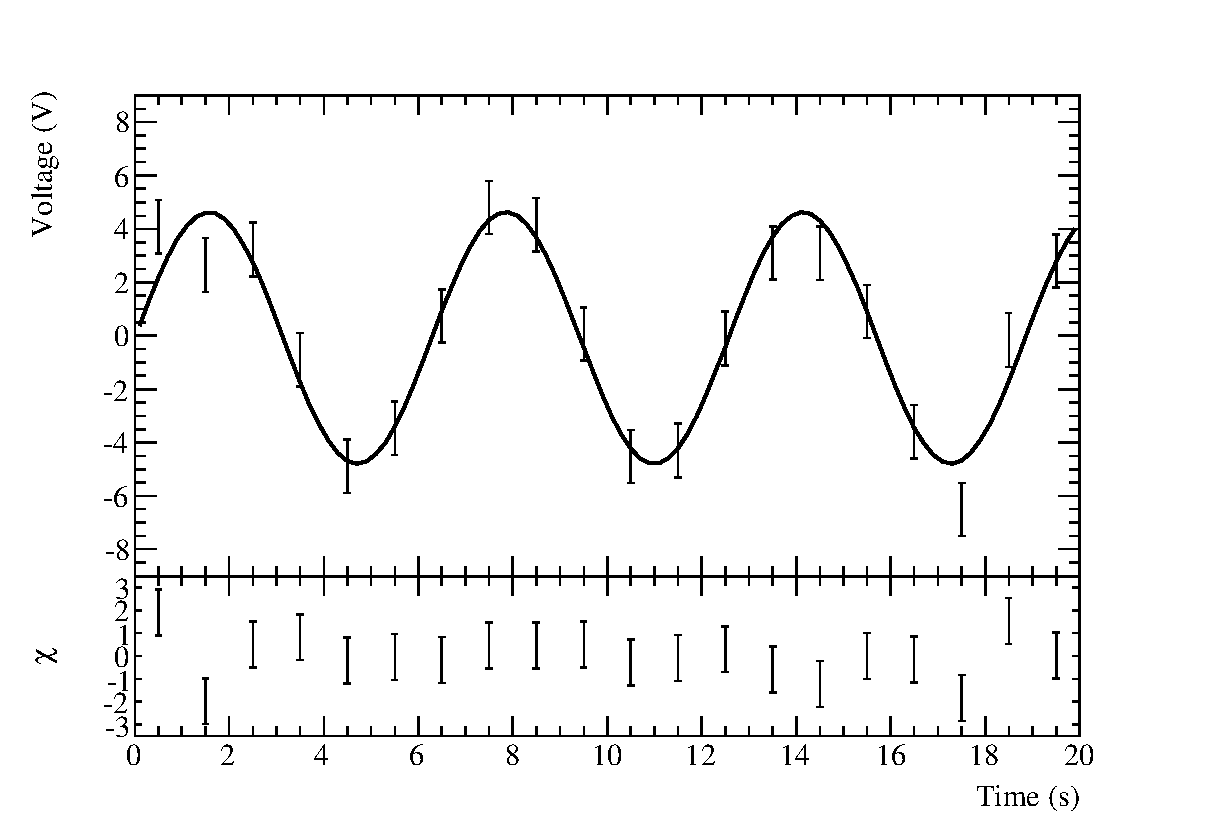
\includegraphics[width=12cm,clip]{fig/residual.eps}
  \caption{コード\ref{code_residual}の出力結果}
  \label{fig_residual_eps}
\end{figure}

\begin{NoFloat}
\lstinputlisting[language=c++,caption=\texttt{residual.C},label=code_residual,numbers=left]{src/residual.C}
\end{NoFloat}

\chapter{統計学の基礎}
\label{chap_Statistics}

実験データの解析作業の目的のひとつは、何らかの物理量をそこから抽出し、その値が統計学的にどれだけ正しいかを評価することです。例えば電子の質量が約511~keVであることを私たちは知っていますが、その真の値がいくつかは誰も知りません\footnote{光速$c$のように299~792~458~$\mathrm{m}/\mathrm{s}$と正確に「定義」されている物理量も存在します。}。物理実験から統計学的な表現で言えるのは、電子質量は
\begin{equation}
  m_\mathrm{e} = 510.998\,946\,1\pm0.000\,003\,1\,\mathrm{keV}
\end{equation}
ということだけです\cite{Patrignani:2016:Review-of-Particle-Physics}。これは510.998~946~1~keVがこれまでの実験でわかった最も良い電子質量の推定値であり、その誤差は0.000~003~1~keVである、もしくは言い方を変えると、約68\%の確率\footnote{より正確には約$68.27$\%であり、これは正規分布の$\pm1\sigma$の範囲に入る確率です。この意味については本章で後述します。}で0.000~003~1~keVの範囲に収まっているという意味です。

ROOTではヒストグラムが自動で計算する平均値や標準偏差といった数値を始めとして、カイ二乗フィットや検定など、様々な統計処理が現れます。これらを理解せずにROOTを使ったりデータ解析を行うと、間違った物理量やその誤差を導出する恐れがありますし、また論文を読んでいても実験データの解釈を正しくできないでしょう。

実験系高エネルギー宇宙物理学の大学院生が必要とする統計学の基本的な情報、またそれをROOTでどのように扱えば良いかをこの章では説明します。

\section{参考書}

この章では非常に基本的なことしか触れませんし、その目的は統計学を学ぶことではなく、ROOTでどのように統計学的な考え方をするかの指針を与えることです。統計学、特に素粒子物理学や宇宙物理学で重要となる統計処理に関しては、いくつかの参考書を挙げるにとどめます。

\begin{enumerate}
  \item \myhref{http://pdg.lbl.gov}{C.~Patrignani and Particle Data Group, ``Review of particle physics'',  {\em Chinese Physics C} {\bf 40}, 100001 (2016)}\\
    素粒子物理学の研究者が2年ごとに編纂している、無料で入手可能な書籍です。この本の確率と統計の章は短いですがよくまとまっています。
  \item \myhref{http://amzn.to/2rzflO2}{Olaf Behnke et~al.``Data Analysis in High Energy Physics: A Practical Guide to Statistical Methods'', Wiley-VCH (2013)}\\
    比較的最近の本で、unfoldingや系統誤差の取り扱い、また天文学での事例など多岐にわたり解説しています。
  \item \myhref{http://amzn.to/2rg6gtJ}{Louis Lyons, ``Statistics for Nuclear and Particle Physicists'', Cambridge University Press, (1989)}\\
    古くからある素粒子・原子核物理向けの統計の教科書です。指導教員の多くが薦めると思います。
  \item \myhref{http://amzn.to/2rg6EIv}{Glenn F. Knoll, ``Radiation Detection and Measurement'', Wiley, 4th edition, (2010)}\\
    放射線計測に関する様々な情報が載っている教科書ですが、簡単な統計の話も取り扱っていて簡単に読めます。
\end{enumerate}

\section{基本的な用語}

\subsection{統計誤差と系統誤差}

一般的に測定値には誤差がつきます。例えばある放射性同位体の放射能を測定することを考えてみましょう。10秒間に100回の崩壊が計数されたとすると、この放射性同位体は10~Bq(ベクレル\footnote{1秒間に平均$N$回崩壊する放射性同位体の放射能を$N$~Bqと表します。})だと言えます。しかしこれは10秒間で崩壊した数がたまたま100回だっただけであり、繰り返し測定を行うと110回だったり90回だったりする可能性もあります。したがって我々が決定できる10~Bqというのはその測定における最良の推定値であり、確率に基づいた誤差が伴います。これを\emphasize{統計誤差(statistical error)}と呼びます。

この例の場合、原理的には測定時間を無限に長くすることで、統計誤差を限りなく小さくすることができます。しかし無限の測定時間を使うことは不可能であり、またその間に放射能自体が変化してしまいます。我々はあらゆる実験において、限られた時間、限られた装置、限られた金銭的・人的資源を使うことしかできませんので、必ず統計誤差と付き合うことになります。

一方、10秒間の測定と簡単に言っても、10秒間を精確に決めるのは困難です。使っている時計が原子時計でもない限り、多少のずれは必ず発生します。10秒間だと思って計測していても、実際には9.9秒だったり10.1秒だったりと、測定系自体に狂いが存在する可能性があります。この場合、10~Bqという推定値は、本当は10.1~Bqだったり9.9~Bqだったりするかもしれません。このような測定系自体の持つ誤差を\emphasize{系統誤差(systematic error)}と呼びます。

例えば上述の時計の場合、時計がどの程度ずれているかというのを、何かしらの外部装置を使って較正し、系統誤差を評価する必要があります。数学の計算さえ間違えなければ、一般的にはあらゆる実験で統計誤差を計算することが可能ですが、系統誤差の評価方法には王道は存在せず、それを解説した書籍も多くないでしょう。本書でも系統誤差については解説しませんので、各実験ごとの系統誤差の評価は、指導教員や先輩に相談しましょう。

\subsection{母集団と標本}

カミオカンデ実験の検出した超新星SN~1987Aからの11個のニュートリノは、SN~1987Aから放出された全てのニュートリノではありません。大マゼラン雲から地球の方向へ飛んできたニュートリノのうち、たまたまカミオカンデで検出された11個に過ぎません。我々は地球上に住んでいるため、SN~1987Aで発生した全方向のニュートリノを観測することはできませんし、また検出器の体積にも限りがあるため、地球に飛来した全てのニュートリノを検出することはできません。

このように物理実験では、発生した全ての事象を観測することができず、その一部だけを観測することによって物理量(例えばこの場合は超新星爆発のエネルギーがニュートリノにどれだけ渡されるかなど)を測定することが多々あります。この一部分のことを\emphasize{標本(sample)}と呼び、それに含まれる事象の数を\emphasize{標本の大きさ(sample size)}と呼びます\footnote{「標本数」(the number of samples)と誤用されることがありますが、これは用語として正しくありません。カミオカンデの他にIMB実験とBaksan実験でもニュートリノが同時に検出されており、標本は合計で3つあることになります。このとき、標本数は3であると言います。}。一方、SN~1987Aで放出されたニュートリノの全てを\emphasize{母集団(population)}と呼びます。すなわち、得られた標本から母集団の性質を推定するわけです\footnote{検出されたニュートリノは検出されやすいニュートリノでもあります。水タンクの有効体積はニュートリノの種類やエネルギーに依存するため、母集団を代表するものではありません。エネルギー依存性などを考慮し、実際には母集団がどのようなものかを推定します。}。

たかだか数百の電話回答を使って1億人の世論を調査できるのは、このような標本から母集団を推定するという統計処理を行うためです。また選挙の出口調査の結果から開票1分で当選確実が出るのも同じ理由です。さらに料理の味見をするときも、全て食べずにひと口舐めれば問題ありません。これらは全て、標本は母集団の性質を反映しているという前提に立っています。

\subsection{平均値と分散と標準偏差}

\subsection{大数の法則}

\subsection{中心極限定理}

\section{様々な確率分布}

ある測定を

\subsection{正規分布}
\subsection{ポアソン分布}

\lstinputlisting[language=c++,float=tb,caption=\texttt{Poisson.C},label=code_Poisson,numbers=left]{src/Poisson.C}

\begin{figure}
  \centering
  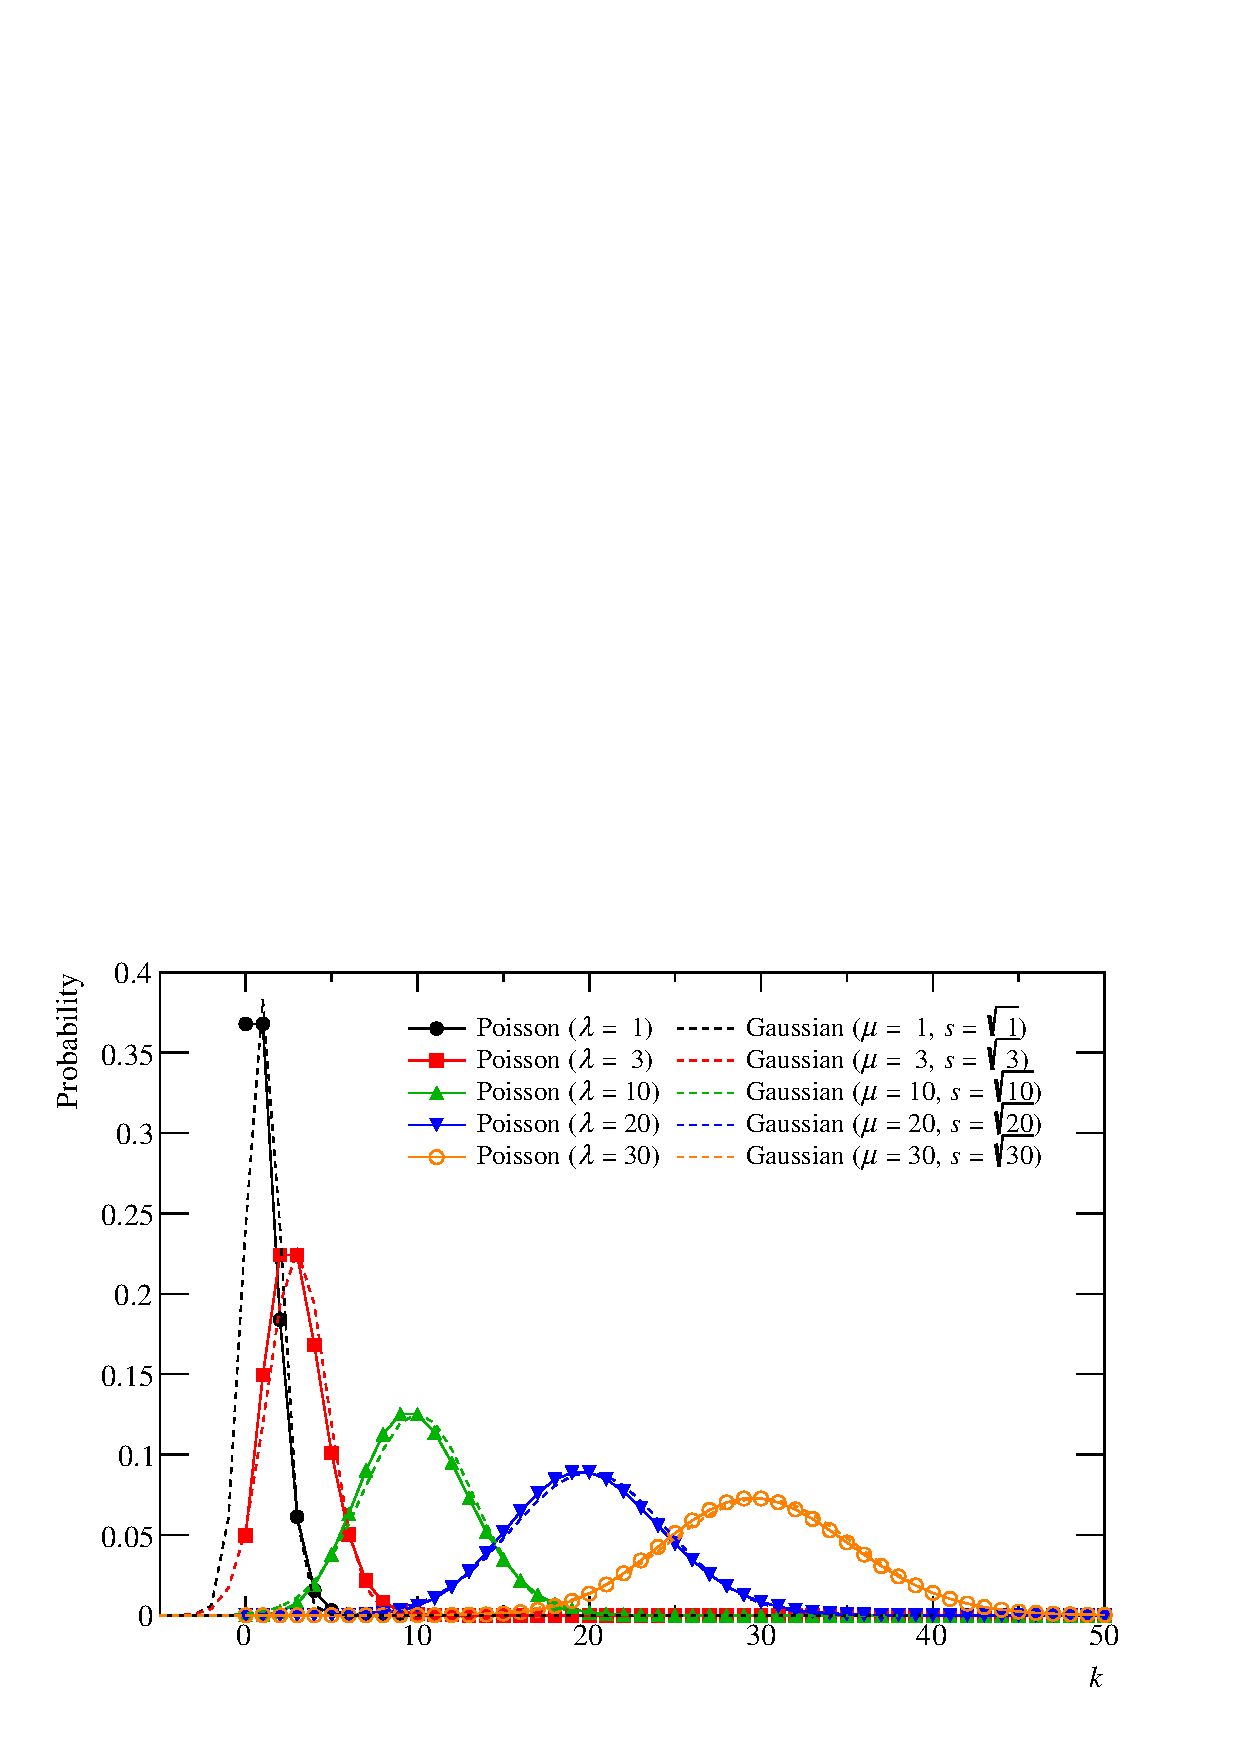
\includegraphics[width=12cm]{fig/Poisson.pdf}
  \caption{様々な平均値を持つポアソン分布と正規分布の比較}
  \label{fig_Poisson}
\end{figure}

\subsection{指数分布}
\subsection{二項分布}
\subsection{カイ二乗分布}


% Reset counters and commands for appendix
\setcounter{chapter}{0}
\renewcommand{\thechapter}{\Alph{chapter}}
\setcounter{equation}{0}
\renewcommand{\theequation}{\Alph{chapter}.\arabic{equation}}
\setcounter{figure}{0}
\renewcommand{\thefigure}{\Alph{chapter}.\arabic{figure}}
\setcounter{table}{0}
\renewcommand{\thetable}{\Alph{chapter}.\arabic{table}}
\appendix

\chapter{パッケージ管理システム}
\label{chap:package}
macOS や Linux にソフトウェアやライブラリを追加インストールする場合、主に3つの方法があります。1つ目はインストーラの付属したソフトウェアをダウンロードしたり、Apple の App Store を経由してインストールする方法です。例えば LINE のパソコン用アプリケーションなどがこれに該当します。また Python もインストーラを配布していますが、この使用はあまり一般的ではないように思います\footnote{\url{https://www.python.org/downloads/mac-osx/}}。

2 つ目はパッケージ管理システム(package management system、package manager)を使用する方法です。これは主に、Python などコマンドラインで使用するソフトウェアのインストールや管理に用いられます。パッケージ管理システムは単に必要なソフトウェアやライブラリをインストールするだけでなく、そのソフトウェアに必要となる他のライブラリを自動的に選択してインストールしたり、バージョンの依存関係を解決してくれたりします。またソフトウェアごとに異なるウェブサイトに情報が散逸することなく、同一のレポジトリに情報が集約され、インストール方法も共通化されているという利点があります。

Mac では後述する Homebrew が 2020 年現在では主流であり\footnote{Mac OS X がリリースされた当初は Fink(\url{http://www.finkproject.org})がもっとも人気があり、その後 MacPorts(\url{https://www.macports.org})に人気が移り、今では Homebrew が主流となりました。}、CentOS~7 では Yum が標準です。また Python に特化したパッケージ管理システムとして pip や conda があるのは第~\ref{chap:Python}~章で説明した通りです。本章では、このHomebrewとYumについて簡単に解説します。

3 つ目の方法はCMakeやconfigureを使ってソフトウェアのビルドとインストールをする方法です。この解説は付録~\ref{chap:configure}を参照してください。

\section{Homebrew}
\label{sec:Homebrew}
Homebrew(ホームブルー)は 2020 年現在、Mac でもっとも人気のあるパッケージ管理システムです\footnote{\url{https://brew.sh}}\footnote{「home brew」は日本語で自家醸造という意味であり、Homebrew に出てくる用語は cask(大樽)や cellar(貯蔵庫)など、酒関係の英語が多いです。}。

まず \url{https://brew.sh} に記述のある通り、Homebrew をインストールしてみましょう\footnote{Homebrewの更新に従いこのコマンドは変更になる可能性があるので、必ず本家の記述を参照してください。}。次のコマンドを管理者権限をもつユーザで実行すると
\begin{lstlisting}[language=bash]
$ /bin/bash -c "$(curl -fsSL https://raw.githubusercontent.com/Homebrew/install/master/install.sh)"
\end{lstlisting}
色々と出てきた後にパスワードを聞かれますので、パスワードを入れて進めてください。
\begin{lstlisting}[language=bash]
==> The Xcode Command Line Tools will be installed.

Press RETURN to continue or any other key to abort
(略)
==> Installing Command Line Tools for Xcode-11.4
==> /usr/bin/sudo /usr/sbin/softwareupdate -i Command\ Line\ Tools\ for\ Xcode-11.4
Software Update Tool


Downloading Command Line Tools for Xcode
Downloaded Command Line Tools for Xcode
Installing Command Line Tools for Xcode
Done with Command Line Tools for Xcode
Done.
==> /usr/bin/sudo /bin/rm -f /tmp/.com.apple.dt.CommandLineTools.installondemand.in-progress
(略)
==> Next steps:
- Run `brew help` to get started
- Further documentation: 
    https://docs.brew.sh
\end{lstlisting}
まず初めに、Command Line Tools for Xcodeと呼ばれるプログラミングに必要となるソフトウェア一式がインストールされます。この中にはコンパイラーなどが含まれ、Appleが配布しているものです。Homebrewとは直接関係ありませんが、Homebrewを動かすのに必要なソフトウェアが入っているため、Homebrewのインストール前にインストールされます。

次にHomebrewを動かすために必要なソフトウェアや設定が順次ダウンロード、インストールされます。\texttt{/usr/local} が作成され、Homebrew 関係のファイルが(ほぼ)全てそこにインストールされるようになります\footnote{例えば MacTeX を入れた場合などは、\texttt{/Library}以下にファイルが置かれる場合があります}。例えば Python~3 を Homebrew でインストールすると \texttt{/usr/local/bin/python3} という場所に置かれます。

Homebrew によって \texttt{/usr/local} 以下に作られるディレクトリは、管理者権限を持つユーザが読み書きできる設定に変更されます。そのため、最初の Homebrew にインストール以降は原則としてパスワードの入力は求められません。

第~\ref{chap:Python}~章で説明したように、Python~3のインストールなどを試してみましょう。

\begin{lstlisting}[language=bash]
$ brew install python3
\end{lstlisting}

他にまず必要なものはCMake、Emacs、MacTeX\footnote{Macに\LaTeX をインストールする方法はいくつかありますが、Homebrew で MacTeX をインストールするのが一番簡単だと思います。} だと思います。MacTeXはダウンロードに時間がかかるので、必要なときでも構いません。
\begin{lstlisting}[language=bash]
$ brew install cmake
$ brew cask install emacs
$ brew cask install mactex
\end{lstlisting}

次のコマンドを実行します。
\begin{lstlisting}[language=bash]
$ echo "Emacs(){\n\t[ -f $1 ] || touch $1\n\topen -a Emacs $1\n}" >> ~/.zshrc
$ source ~/.zshrc
$ which Emacs
Emacs () {
	[ -f ] || touch
	open -a Emacs
}
\end{lstlisting}
これで、\texttt{Emacs}というコマンド(実際は関数)で\texttt{/Applications/Emacs.app}を起動できるようになりました。

macOS Catalinaの場合、Emacsをまともに動作させるには少し修正を加える必要があります\footnote{2020年4月19日現在の情報のため、不正確な記述になる可能性があります。}。HomebrewでEmacs.appが\texttt{/Applications/Emacs.app}にインストールされた後、\textbf{まずEmacs.appを起動}してください。\cmdkey\,Qで一度終了し、次のコマンドをTerminal.appから実行してください。

\begin{lstlisting}[language=bash]
$ cd /Applications/Emacs.app/Contents/MacOS 
$ mv Emacs Emacs-launcher
$ mv Emacs-x86_64-10_14 Emacs
$ cd ..
$ rm -rf _CodeSignature
$ cd
\end{lstlisting}

\section{\texttt{yum}}

CentOS~7などの Red Hat Enterprise Linux(RHEL)派生の Linux ディストリビューション(いわゆる「RHEL クローン」)では、Yum(Yellowdog Updater Modified、ヤム)というパッケージ管理システムが多く使われています。macOS の Homebrew とは違いシステム標準で組み込まれています。そのためCentOS の OS インストール時点で追加パッケージを選択するのと、OS インストール後に \texttt{yum} コマンドで追加インストールのは基本的に同じことだと思ってください。

CentOS~7やRHELは比較的「枯れた」ソフトウェアを提供する傾向にあります。つまり、あまり新しいソフトウェアのバージョンを取り込まず、実績と安定性を重視して古いバージョンを使用します。そのため Python~3 など新しいソフトウェアは、標準の Yum のレポジトリからは取得できません。そこで、第~\ref{chap:Python}~章で説明したように、場合によってレポジトリを追加する必要があります\footnote{追加レポジトリは多数ありますので、ここに例として示す\url{https://centos7.iuscommunity.org/ius-release.rpm}に限りません。}。

\begin{lstlisting}[language=bash]
$ sudo yum install -y https://centos7.iuscommunity.org/ius-release.rpm
\end{lstlisting}

例えば Python~3をインストールするには、次のようにします\footnote{\texttt{yum search python3}を実行すると、\texttt{python36u-devel}と\texttt{python36u}が見つかるはずです。この例のように\texttt{-devel}がついているものは、ソフトウェア開発で必要となるヘッダーファイルなども一緒にインストールします。例えばROOTのビルド時にPythonのヘッダーファイルも必要となりますので、\texttt{-devel}のほうをインストールするようにしてください。}。\texttt{/usr}以下に新たにファイルを追加するため、管理者権限で実行する必要があります。

\begin{lstlisting}[language=bash]
$ sudo yum install python36u-devel
$ which python3.6
/usr/local/python3.6
\end{lstlisting}

また ROOT のビルドで必要となるCMakeは3.6以上ですので、\texttt{cmake3}を入れてください。

\begin{lstlisting}[language=bash]
$ sudo yum install cmake3
$ which cmake3
/usr/bin/cmake3
$ cmake3 --version
cmake3 version 3.14.6

CMake suite maintained and supported by Kitware (kitware.com/cmake).
\end{lstlisting}

\chapter{\LaTeX 環境の構築}
\label{chap:LaTeX}

\LaTeX とは何かということについては、ここでは詳しく説明しません。大雑把には、テキストファイルで作られた文書をそこそこ綺麗な出力で PDF などに自動で組版(くみはん)してくれるソフトウェアです。この文書も \LaTeX で作られています。

\LaTeX を知らなくても修士論文は書けますが、宇宙や素粒子関連の業界では、ほとんどの人が \LaTeX を使って修士論文を書きます(実際には日本語対応の \pLaTeX)。また同様に投稿論文も \LaTeX で書くことがほとんどですので(実際には PDF の生成が簡単な pdf\LaTeX)、多くの物理学徒が避けては通れない道具です。実際に修士論文を \pLaTeX で書く場合の例としては、手前味噌ですが「修士論文 LaTeX テンプレート|名古屋大学宇宙地球環境研究所の理学系修士学生用」\footnote{\url{https://github.com/akira-okumura/MasterThesisTemplate}}が参考になると思います。

\LaTeX のインストール方法は様々であり、インターネット上の情報もバラバラです。また古い情報も混在しているため、筆者も何が正しいのか、何がお勧めなのかよく分かりません。しかし、ここで示すやり方が「正しそうに思える」ので、ひとつの例として挙げます。この情報は 2019 年 4 月現在のものです。TeXLive などの 2019 年版が出たら、適宜読み替えてください\footnote{2019 年 4 月現在、2018 年版が出ています。}。

macOS でも CentOS~7 でも、合計で 5~GB くらいのファイルをインストールします。ダウンロードに 1 時間以上かかったり、パソコンの空き領域を食いつぶしたりするので注意してください。

\section{macOS での MacTeX のインストール}

macOS で LaTeX 環境を構築するには、Homebrew で MacTeX というパッケージを追加するのが簡単です。MacTeX は TeXLive という \LaTeX ディストリビューションに Mac 固有のアプリケーションなどを追加したものです。例えば Keynote などに数式を入れたいときに便利な LaTeXiT、文献管理ソフトの BibDesk、TeX 統合環境の TeXShop などが \texttt{/Applications} にインストールされます\footnote{筆者はこのうち LaTeXiT と BibDesk のみ常用しています。}。

いつも通り単純に次のコマンド一発でいけます。ただし、\texttt{brew install} ではなく \texttt{cask} というのが間に挟まっているのを注意してください。
\begin{lstlisting}[language=bash]
$ brew cask install mactex
\end{lstlisting}

次のコマンドを実行した際に
\begin{lstlisting}[language=bash]
$ sudo tlmgr paper
\end{lstlisting}
もしもページの大きさの設定が次のように letter(21.59~cm~$\times$~27.94~cm)\footnote{アメリカで一般的に使われる印刷用紙の大きさです。}と表示される場合、
\begin{lstlisting}
Current context paper size (from /usr/local/texlive/2018/texmf-config/tex/context/user/cont-sys.tex): letter
Current dvipdfmx paper size (from /usr/local/texlive/2018/texmf-config/dvipdfmx/dvipdfmx.cfg): letter
Current dvips paper size (from /usr/local/texlive/2018/texmf-config/dvips/config/config.ps): letter
Current pdftex paper size (from /usr/local/texlive/2018/texmf-config/tex/generic/config/pdftexconfig.tex): letter
Current psutils paper size (from /usr/local/texlive/2018/texmf-config/psutils/paper.cfg): letter
Current xdvi paper size (from /usr/local/texlive/2018/texmf-config/xdvi/XDvi): letter
\end{lstlisting}
次のコマンドで A4 サイズ(21.0~cm~$\times$~29.7~cm)に設定を変更してください。
\begin{lstlisting}[language=bash]
$ sudo tlmgr paper a4
\end{lstlisting}

macOS で \LaTeX\ を使う場合、初期設定ではおそらく IPA 明朝と IPA ゴシックというフォントが使用されます。しかし macOS に同梱されているヒラギノフォント(ヒラギノ明朝およびヒラギノ角ゴシック)を使うと PDF の仕上がりが良くなります(可読性の高い綺麗なフォントが埋め込まれます)ので、仕上がりにこだわりたい人はヒラギノフォントを埋め込む設定を行なってください。この作業は macOS のバージョンや TeXLive のバージョンによって異なりますので、\url{https://doratex.hatenablog.jp/entry/20190502/1556775026}などを参考にしてください。

\section{CentOS~7 での TeXLive 2018 のインストール}

\url{https://www.tug.org/texlive/quickinstall.html}を参考に、まずはネットワーク越しにインストール\footnote{必要なファイルをインストーラとともに最初に落としてくるのではなく、インストーラを実行した後に必要ファイルをダウンロードしてくる方法。}するためのコマンドをダウンロードし展開します。

\begin{lstlisting}[language=bash]
$ cd
$ curl -O -L http://mirror.ctan.org/systems/texlive/tlnet/install-tl-unx.tar.gz
$ tar zxvf install-tl-unx.tar.gz
$ cd install-tl-20190227/
\end{lstlisting}

この展開したディレクトリの中にインストーラがあるので、これを管理者権限で実行します。そうすると次のように色々と表示されるので、i を入力してインストールを進めましょう。もしカスタマイズしたい人は、英語の説明に従ってください。

\begin{lstlisting}[language=bash]
$ sudo ./install-tl
Loading ftp://ftp.u-aizu.ac.jp/pub/tex/CTAN/systems/texlive/tlnet/tlpkg/texlive.tlpdb
Installing TeX Live 2018 from: ftp://ftp.u-aizu.ac.jp/pub/tex/CTAN/systems/texlive/tlnet (verified)
Platform: x86_64-linux => 'GNU/Linux on x86_64'
Distribution: net  (downloading)
Using URL: ftp://ftp.u-aizu.ac.jp/pub/tex/CTAN/systems/texlive/tlnet
Directory for temporary files: /tmp/bDF8hSU8Tp

======================> TeX Live installation procedure <=====================

======>   Letters/digits in <angle brackets> indicate   <=======
======>   menu items for actions or customizations      <=======

 Detected platform: GNU/Linux on x86_64
 
 <B> set binary platforms: 1 out of 17

 <S> set installation scheme: scheme-full

 <C> set installation collections:
     40 collections out of 41, disk space required: 5806 MB

 <D> set directories:
   TEXDIR (the main TeX directory):
     /usr/local/texlive/2018
   TEXMFLOCAL (directory for site-wide local files):
     /usr/local/texlive/texmf-local
   TEXMFSYSVAR (directory for variable and automatically generated data):
     /usr/local/texlive/2018/texmf-var
   TEXMFSYSCONFIG (directory for local config):
     /usr/local/texlive/2018/texmf-config
   TEXMFVAR (personal directory for variable and automatically generated data):
     ~/.texlive2018/texmf-var
   TEXMFCONFIG (personal directory for local config):
     ~/.texlive2018/texmf-config
   TEXMFHOME (directory for user-specific files):
     ~/texmf

 <O> options:
   [ ] use letter size instead of A4 by default
   [X] allow execution of restricted list of programs via \write18
   [X] create all format files
   [X] install macro/font doc tree
   [X] install macro/font source tree
   [ ] create symlinks to standard directories

 <V> set up for portable installation

Actions:
 <I> start installation to hard disk
 <P> save installation profile to 'texlive.profile' and exit
 <H> help
 <Q> quit

Enter command: i
\end{lstlisting}

かなり時間がかかりますが、必要なファイルを全てダウンロードし終えると、最後に環境変数を設定するように指示が出ます。

\begin{lstlisting}
Installing to: /usr/local/texlive/2018
Installing [0001/3752, time/total: ??:??/??:??]: 12many [376k]
Installing [0002/3752, time/total: 00:04/08:25:18]: 2up [66k]
Installing [0003/3752, time/total: 00:05/08:57:54]: Asana-Math [482k]
Installing [0004/3752, time/total: 00:07/05:59:39]: ESIEEcv [137k]
(略)
Add /usr/local/texlive/2018/texmf-dist/doc/man to MANPATH.
Add /usr/local/texlive/2018/texmf-dist/doc/info to INFOPATH.
Most importantly, add /usr/local/texlive/2018/bin/x86_64-linux
to your PATH for current and future sessions.
\end{lstlisting}

これに従い、\texttt{\~{}/.bashrc}や\texttt{\~{}/.zshrc}に次の 3 行を追加します\footnote{インストールの年によって \texttt{2018} が \texttt{2019} に変わっていたりする可能性があるので、実際の出力に従ってください。}。

\begin{lstlisting}[language=bash]
export MANPATH=/usr/local/texlive/2018/texmf-dist/doc/man:$MANPATH
export INFOPATH=/usr/local/texlive/2018/texmf-dist/doc/info:$INFOPATH
export PATH=/usr/local/texlive/2018/bin/x86_64-linux:$PATH
\end{lstlisting}

\section{動作確認}

新しいターミナルのウィンドウを開き、次のコマンドで \texttt{RHEA.pdf}(この文書)が生成できるかを確認しましょう。

\begin{lstlisting}[language=bash]
$ git clone https://github.com/akira-okumura/RHEA.git
$ cd RHEA
$ ls
Makefile  RHEA.bib  RHEA.tex  misc      tex
README.md RHEA.bst  fig       src
$ make
$ ls
Makefile  RHEA.bbl  RHEA.bst  RHEA.out  RHEA.toc  src
README.md RHEA.bib  RHEA.dvi  RHEA.pdf  fig       tex
RHEA.aux  RHEA.blg  RHEA.log  RHEA.tex  misc
$ open RHEA.pdf # macOS の場合
$ xdg-open RHEA.pdf # Linux の場合
\end{lstlisting}

\chapter{Macでの研究環境の構築}
\label{chap:Mac}

ここでは、Macで研究環境を構築する際に最低限やるべきこと、知っておくべきことを説明します。Macに限らずWindowsやLinuxでも、計算機環境の設定は個々人の好みや研究内容によって大きく変わります。そのため、ここに書くことは参考程度にとどめて下さい。この章での説明は、macOS Catalina(10.15.4)を前提に書かれており、また使用するスクリーンショットも同環境のものです。macOS Mojave(10.14)以前では多少異なる可能性があるので注意してください。

\section{最低限知っている必要のあるアプリケーションと機能}

\subsection{Dock}
図~\ref{fig:Catalina}は、macOS Catalinaに初めてログインした際に表示される画面です。一番上にあるのがメニューバー(menu bar)、一番下にあるのがDock(ドック)です。Windowsと異なり、メニューバーは常に画面上部に表示され、アプリケーションを起動してもそのウィンドウごとには表示されません。

Dockは頻繁に使うアプリケーションや、起動中のアプリケーションを表示するために使われます。デフォルトの状態では常に表示されて邪魔なため、右の方にある仕切り線を2本指クリックもしくは2本指タップすることで、表示・非表示を切り替えることができます。非表示にした場合、カーソルを近づけたときにだけ現れます。
\begin{figure}
  \centering
  \includegraphics[scale=0.25]{fig/Catalina.png}
  \caption{macOS Catalinaの初期画面}
  \label{fig:Catalina}
\end{figure}

\subsection{Finder}
\label{subsec:Finder}
FinderはMacの中にあるファイル、フォルダ、アプリケーションなどを表示するために使用するアプリケーションです。WindowsのFile Explorerに相当します。Macに接続したUSBメモリや、ネットワーク上の共有デバイスなどもFinderから操作します。

DockからFinderを最初にクリックすると、図~\ref{fig:Finder_recents}のように最近使った項目(Recents)が表示されます。最初は何もまだ使っていないので、中身は空っぽです。

\begin{figure}
  \centering
  \subfigure[]{
    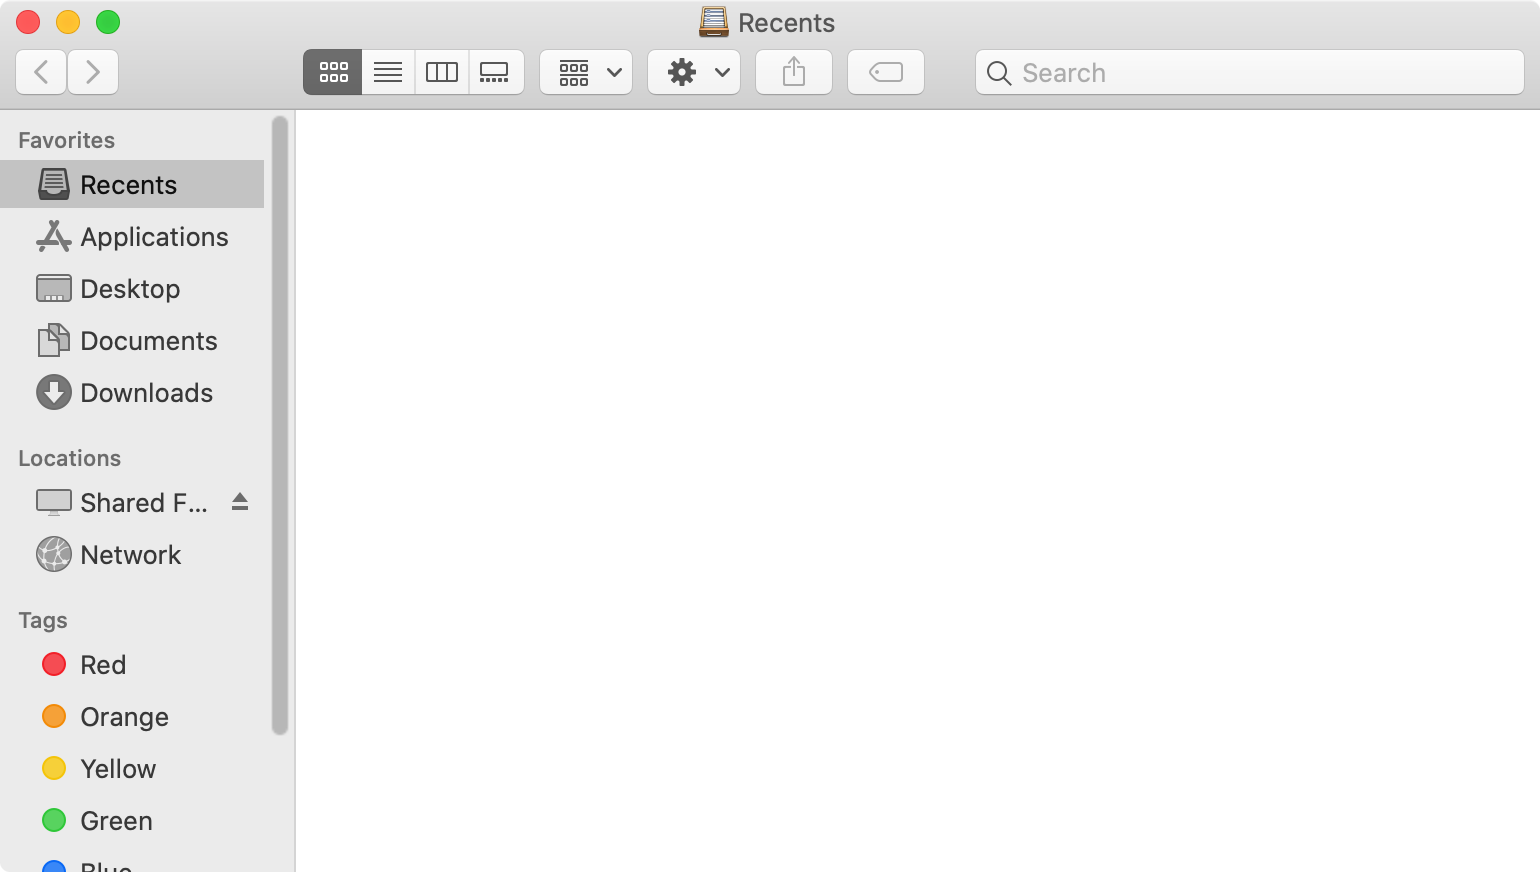
\includegraphics[width=.48\textwidth,clip]{fig/Finder_recents.png}%
    \label{fig:Finder_recents}%
  }\hfill%
  \subfigure[]{%
    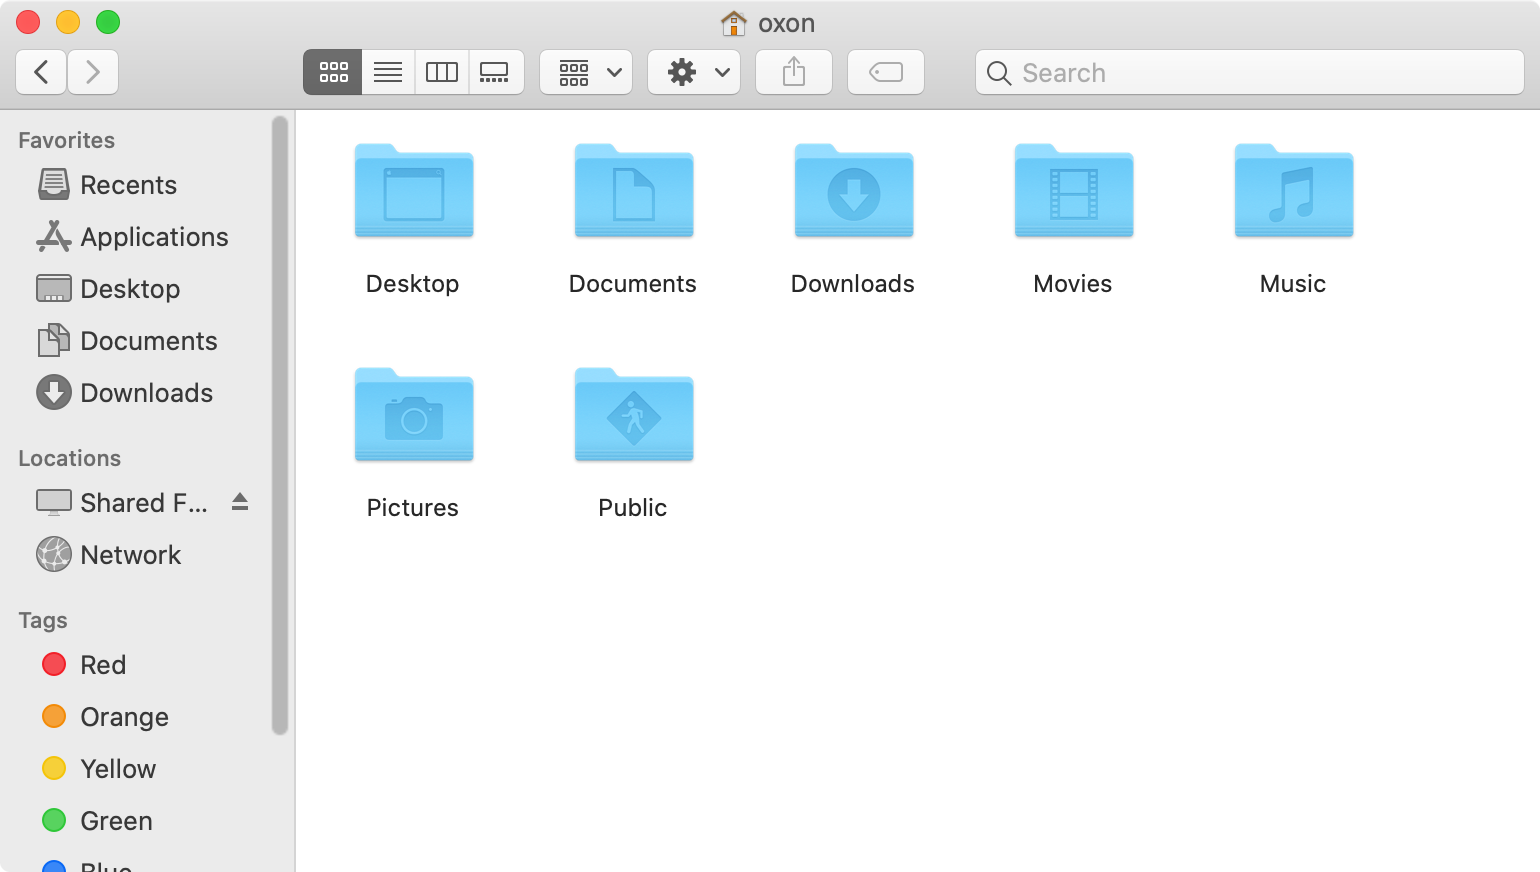
\includegraphics[width=.48\textwidth,clip]{fig/Finder_home.png}%
    \label{fig:Finder_home}%
  }
  \subfigure[]{%
    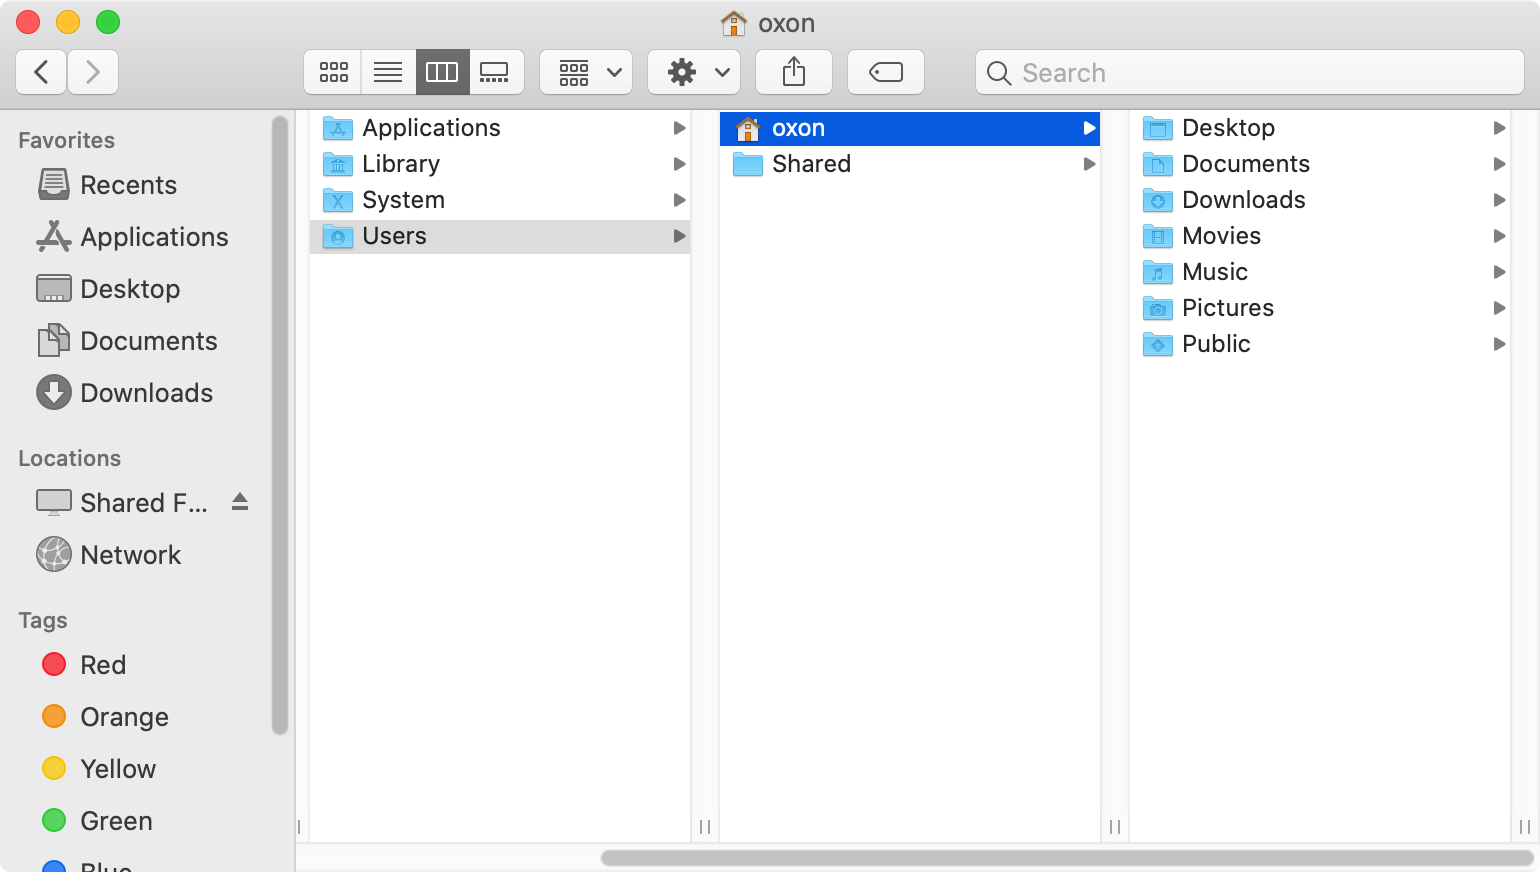
\includegraphics[width=.48\textwidth,clip]{fig/Finder_column.png}%
    \label{fig:Finder_column}
  }\hfill%
  \subfigure[]{%
    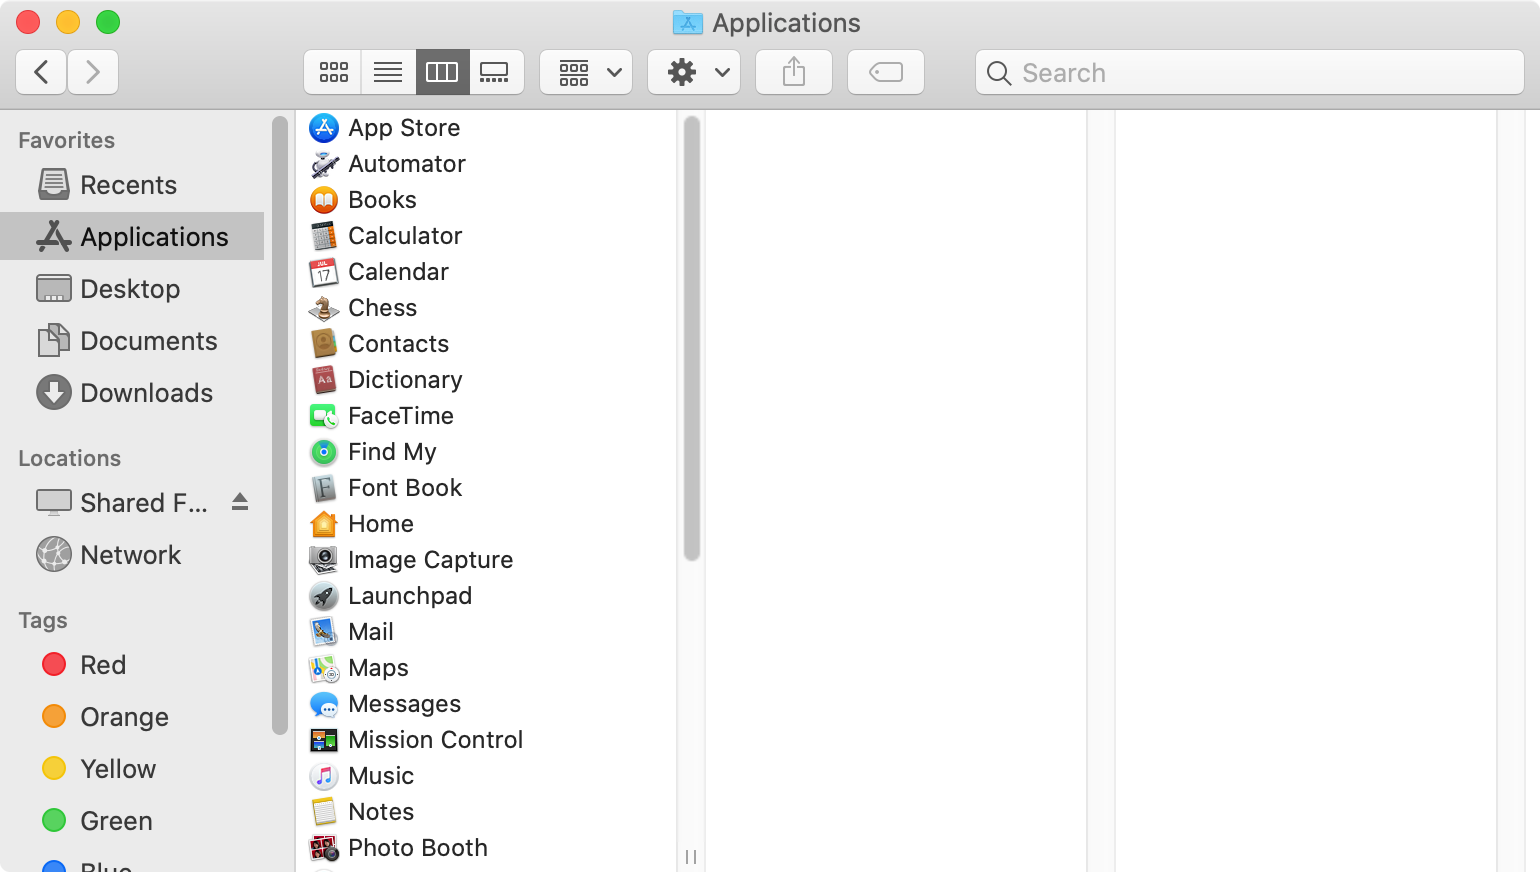
\includegraphics[width=.48\textwidth,clip]{fig/Finder_applications.png}%
    \label{fig:Finder_applications}%
  }
  \caption{Finderの表示例。(a) Recentsの表示。(b)ホームを表示したところ。(c)ホームをカラム表示にしたもの。(d) Applicationsの表示。}
\label{fig:Finder}
\end{figure}

次にシフトキー(Shift)とコマンドキー(\cmdkey\,の記号)とHキーを同時に押すと(\shiftkey\cmdkey\,Hや、Cmd+Shift+Hと表記します)、図~\ref{fig:Finder_home}のようにホーム(Home)に移動します。ホームは個々のユーザが使用できる領域で、実験データや解析プログラムなどは、原則としてホームの下に置きます。アカウント名が例えばoxonの場合、このホームフォルダのパスは\texttt{/Users/oxon}です。

キーボードから複数のキーの組み合わせで、ある特定の動作をさせるものを、キーボードショートカット(keyboard shortcut)と呼びます。Windowsではコントロールキー(Control key)中心ですが、Macの場合はコマンドキー(Command key、\cmdkey)が中心です。例えばコピーやペーストなどのショートカットは、\cmdkey\,Cと\cmdkey\,Vです。

通常、ショートカットはメニューバーから辿ることもできます。既に行ったホームへの移動は、メニューバーの「Go」から「Home」選択すると同じ動作をします。メニューの中にある文字列の右側にショートカットが記載されており、コマンドキー(\cmdkey)、シフトキー(\shiftkey)、オプションキー(\optkey)、コントロールキー(\ctlkey)、デリートキー(\delkey)などと組み合わされたものが表示されています。

さて、Finderの表示がこのままだと移動が不便なので、\cmdkey\,3を押してみましょう。これで表示形式がカラム(column)表示に切り替わります。アイコンが小さくなり情報量が増え、ディレクトリ階層のどこにいるかも分かりやすくなります。

図~\ref{fig:Catalina}のデスクトップ(desktop)\footnote{グラフィカルな画面を持つパーソナルコンピュータが登場した1980年代、その概念を分かりやすくするため机を連想させる用語が導入されました。デスクトップとは机の上であり、そこに様々な書類が置かれたり、また複数の書類をまとめてしまっておくためにフォルダという言葉が使われました。}はデスクトップピクチャ(desktop picture)\footnote{Macでは「壁紙」という言葉ではなくデスクトップピクチャと呼ぶのが正統です。壁紙やwallpaperという言葉は、Windows由来です(窓と壁という連想)。}が表示されているだけで、ファイルは置かれていません。しかしこのデスクトップもフォルダのひとつになっていて、何かしらのファイルをデスクトップに置くと、図~\ref{fig:Finder_column}に表示されているDesktop(\texttt{/Users/oxon/Desktop})にそのファイルが表示されます。試しに\cmdkey\,\shiftkey\,3を押してみてください。これでスクリーンショット(screenshot)が撮影され、デスクトップにPNG画像として保存されるはずです。

次に、\cmdkey\,\shiftkey\,Aを押してみてください。図~\ref{fig:Finder_applications}に表示が切り替わるはずです。macOSにインストールされるアプリケーションの多くはこのApplicationsフォルダ(\texttt{/Applications})に配置されます。ただし、Finderのようにシステムに非常に近い動作をするような一部のアプリケーションは、ここには置かれていません。

\subsection{System Preferences}
System PreferencesはユーザがMacの設定を好みに変更するためのアプリケーションです。日本語環境では「システム環境設定」と呼ばれます。起動すると図~\ref{fig:SystemPreferences}が開き、様々な設定項目を変更することができます。
\begin{figure}
  \centering
  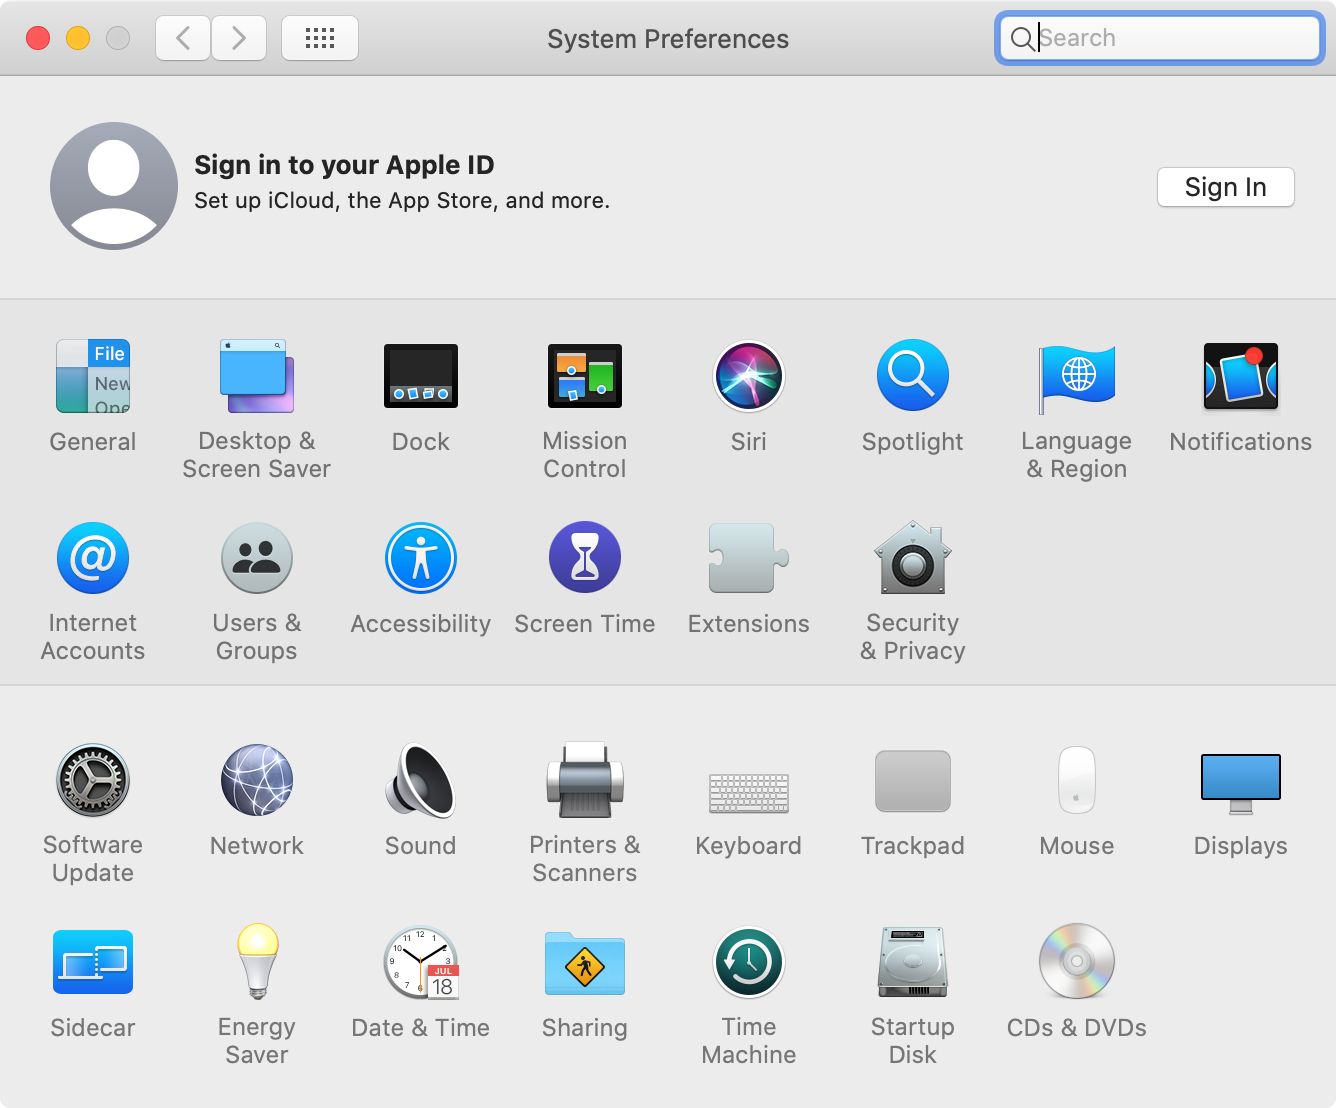
\includegraphics[scale=0.35]{fig/SystemPreferences.png}
  \caption{System Preferencesの画面}
  \label{fig:SystemPreferences}
\end{figure}

\subsection{Safari}
SafariはmacOS、iOS(iPhone)、iPadOS(iPad)に搭載されている、標準のウェブブラウザ(web browser)です。通常の使用であればSafariでも問題ありませんが、より機能拡張したい、WindowsやLinuxと同じ環境に揃えたいという場合は、Google Chromeなど他社製のブラウザを追加インストールすることもできます。

Safariを使用してROOTなどのファイルをインターネットからダウンロードした場合、図~\ref{fig:Finder_column}に表示されているDownloadsフォルダ(\texttt{/Users/oxon/Downloads})に保存されます。
\subsection{Mail}
MailはmacOS標準の電子メールクライアント(E-mail client)\footnote{クライアントとは、サーバと情報のやり取りをするソフトウェアを指すコンピュータ用語です。}です。WindowsやLinuxと環境を揃えたい場合は、Thunderbirdなど他社製のクライアントを追加インストールすることもできます。電子メールクライアントは比較的枯れた技術ですので、特に強い好みがない場合は、Mailを使っておけば十分だと思います。

Mailは一般名詞であり、会話中でも文章中でも一般名詞との区別が困難なことから、Mail.appやApple Mailと呼ぶことが頻繁にあります。ここで、\texttt{.app}はmacOSでアプリケーションに使われる拡張子です。

\subsection{Spotlight}
Dockに表示されているアプリケーション以外にも、\ref{subsec:Finder}~節で説明したように\texttt{/Applications}に多くのアプリケーションがあります。このようなアプリケーションをクリックで起動したりするのは面倒です。そこで、macOS標準の検索機能であるSpotlightを使用してみましょう。

\cmdkey\,Spaceを押してみてください\footnote{図~\ref{fig:Catalina}にあるSpotlightのアイコンをクリックするのでも同じように機能します。}。図~\ref{fig:Spotlight}が現れ、そこに例えば「Finder」と入力すると、図~\ref{fig:Spotlight_results}のように検索結果が現れます。ここでリターンキー(\returnkey)を押すと、Finderを開こうとするため、Finderがアクティブの状態(全てのアプリケーションよりも手前に来る状態)になります。また\cmdkey\,\returnkey\,を押すと、その項目をFinder上で表示します。Finder.appの実体が\texttt{/System/Library/CoreServices/}にあることが分かります。

\begin{figure}
  \centering
  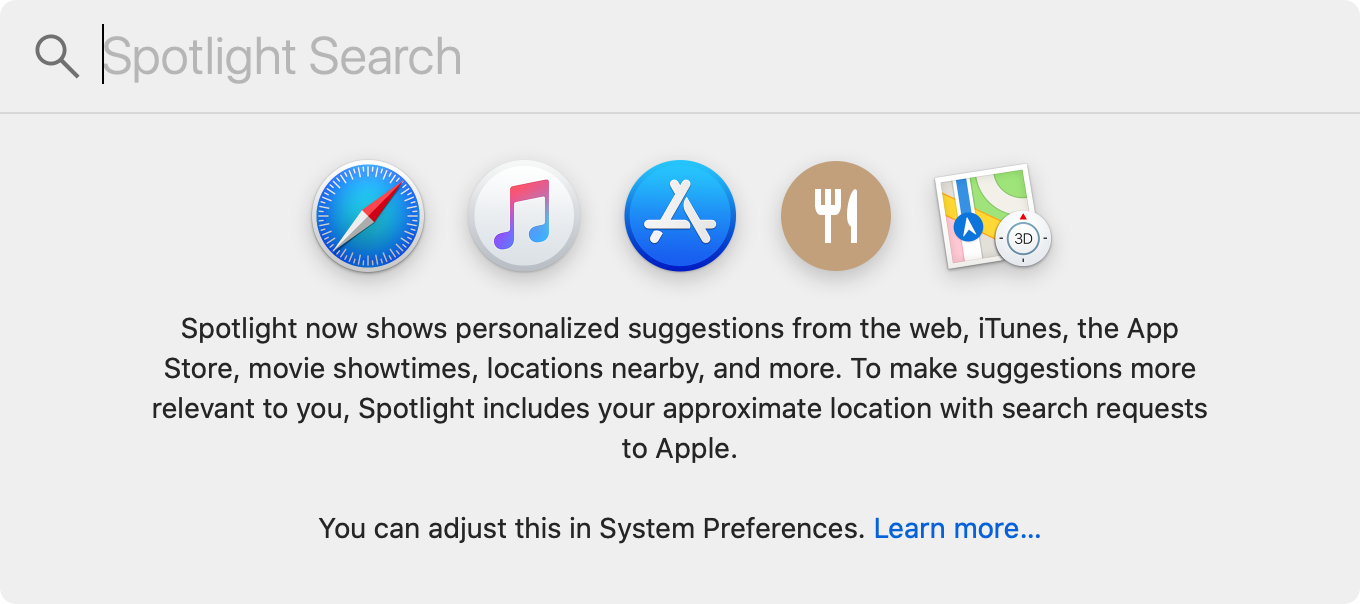
\includegraphics[scale=0.35]{fig/Spotlight.png}
  \caption{Spotlightの画面}
  \label{fig:Spotlight}
\end{figure}
\begin{figure}
  \centering
  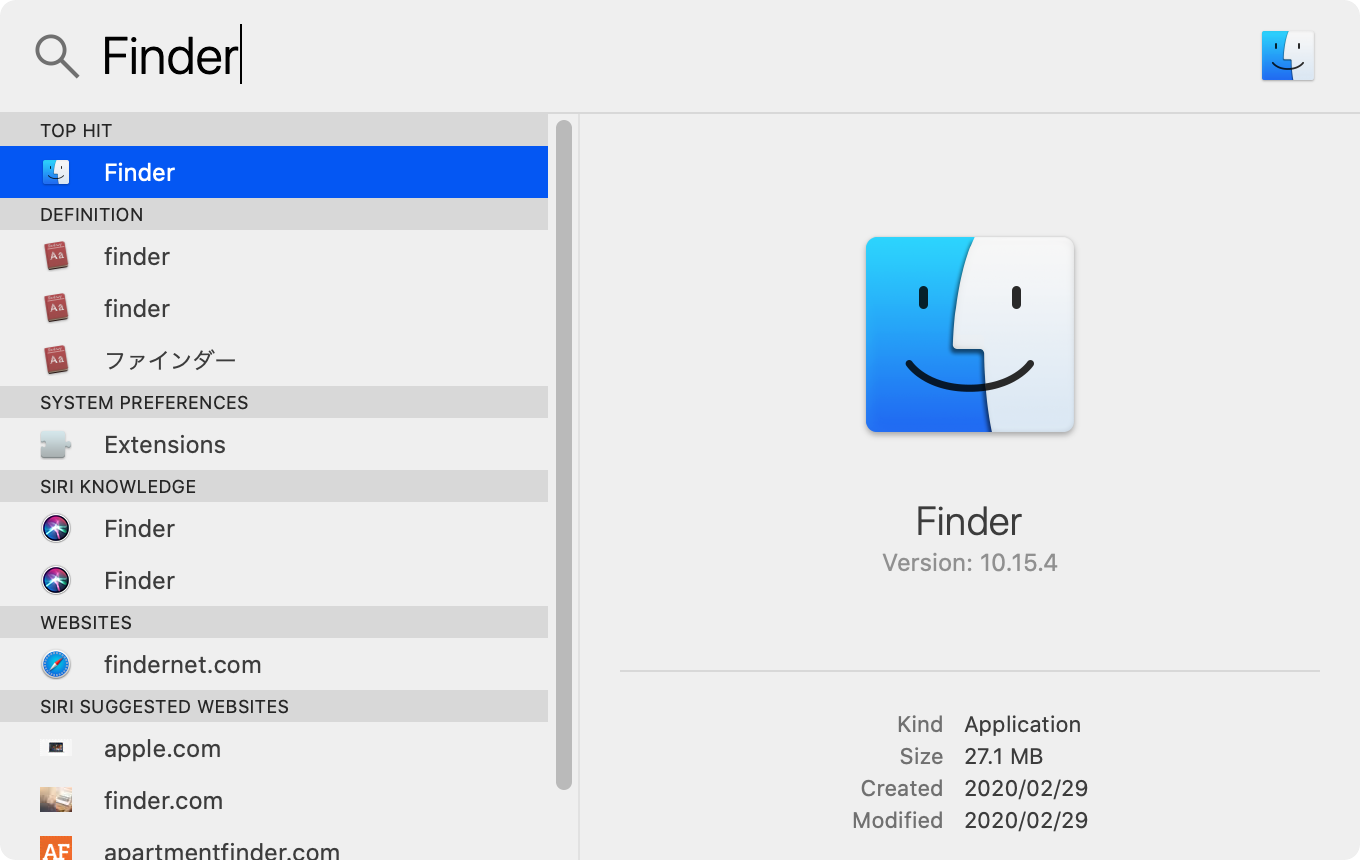
\includegraphics[scale=0.35]{fig/Spotlight_results.png}
  \caption{Spotlightの検索結果の例}
  \label{fig:Spotlight_results}
\end{figure}

\subsection{App Store}
macOSに新しくソフトウェアをインストールするには、大別して4つの方法があります。App Storeを利用する方法(Keynoteなど)、インターネット上でApp Store以外の場所からアプリケーション本体やインストーラをダウンロードしてくる方法(Google Chromeなど)、Homebrewなどのパッケージ管理システムを使用する方法(Pythonなど)、ソースコードをダウンロードして自分でビルドする方法(ROOTなど)です。

macOSのApp Storeは、iPhoneやiPadのApp Store、Android端末上でのGoogle Play、WindowsのMicrosoft Storeと同様のものです。無料のものも有料のものも、次節で説明するApple IDを使用することでインストールすることができます。Microsoft Officeに相当するApple製のPages、Keynote、Numbersなども、このApp Storeからインストールします。

\subsection{Apple IDとiCloud}

App Storeでアプリケーションをインストールする場合、有料・無料を問わずApple IDと呼ばれるアカウントを作成する必要があります\footnote{\url{https://support.apple.com/ja-jp/HT204316}を参照。}。有料ソフトウェアを購入する場合は、クレジットカード情報をさらに付与する必要があります。

Apple IDを登録することで、iCloudというAppleの提供するクラウドサービスを使用できるようになります。研究に関係するところでは、例えば複数のMacでのファイルの同期、Apple ID同士を使っての画面共有などが利用できるようになります。

\subsection{Terminal}
ターミナル(Terminal)はプログラミングやデータ解析などをするときに必要となるアプリケーションです。映画やドラマなどでハッカーやクラッカーが黒い画面に向かってキーボードを連打しているのは、ターミナルで作業をしています。Mailと同じくTerminalは一般名詞であり、macOSに限らずターミナル機能を有する環境は多数あるため、macOSのTerminalアプリケーションを指す場合は、Terminal.appと表記する場合があります。

ターミナルとは「端末」のことです。コンピュータ用語で、ユーザが入出力を行うための装置を指します。現在のようにグラフィカルな操作ができなかった昔のコンピュータでは、ターミナルからコンピュータに指示を出し(入力)、その結果(出力)を受け取るという作業をしていました。プログラミングやデータ解析などでは、今でもターミナルを利用したほうが作業効率が良いため、使われ続けています。

Terminal.appはDockには入っておらず、\texttt{/Applications/Utilities/}にあります。Spotlight(\cmdkey\,Space)を使って起動してみましょう。図~\ref{fig:Terminal}のような画面が現れるはずです。
\begin{figure}
  \centering
  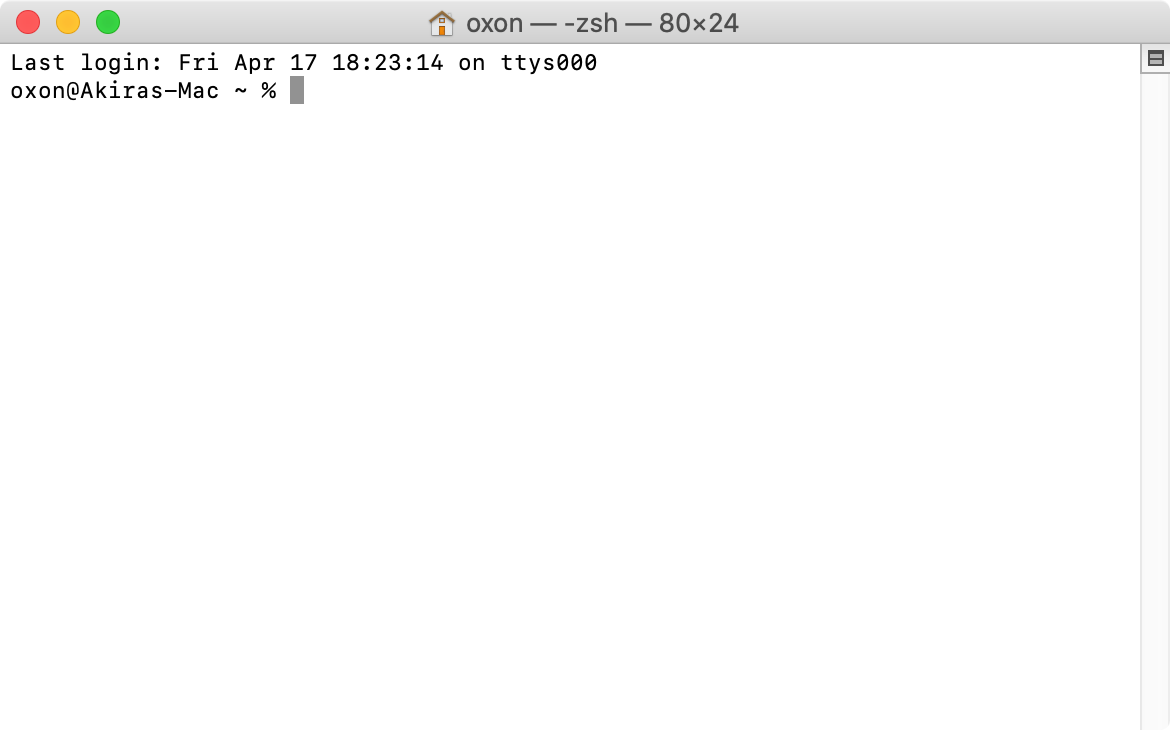
\includegraphics[scale=0.35]{fig/Terminal.png}
  \caption{Terminalの初期画面}
  \label{fig:Terminal}
\end{figure}

\subsection{Time Machine}
Time MachineはmacOSの自動バックアップの仕組みです。設定することで、外付けハードディスクやTime Capsule(タイムカプセル)\footnote{Appleが販売していた、内蔵ハードディスク付きのWi-Fiルータ。}にバックアップを作成することができます。

\subsection{アプリケーションの切り替え}
起動しているアプリケーションを切り替えるのは、\cmdkey\,Tabで行います。同一アプリケーション内でウィンドウを切り替えるのは、\cmdkey\,`で行います。

\section{英語環境にする}
日本の研究室でMacを使う場合、OSの言語環境を日本語にしている人が多いでしょう。しかしMacを研究で使う場合には英語環境に変更することを強くお勧めします。大きく四つの理由があるからです。

まず第一に、インターネット上のMac関係の情報の多くが英語で書かれており、英語で検索した場合に見つかる情報の量と質は日本語の情報を圧倒するからです。使っているMacで何か問題が生じた場合にエラーメッセージが日本語で表示されていると、それを検索語にしても辿り着ける情報には限りがあります\footnote{日本語入力や\LaTeX 関係などの情報だと日本語特有の問題も発生しうるので、そこは臨機応変に対応して下さい。}。Apple社はアメリカの企業でありMacユーザの多くが北米に集中しています。そのためMac関連の情報のやり取りの多くは英語でなされています。これはMacに限らずコンピュータ関係全般に言えます\footnote{恐らく唯一の例外がRubyというプログラミング言語です。これは日本人により開発されたものが世界に広がった希有な例です。}

第二に、あなたは日本人のみと共同研究をするわけではないからです。もしあなたのMacの画面を外国人が見ながら、もしくはあなたが外国人のMacの画面を見ながら作業する時に、OSが英語環境になっていたほうが意志疎通が簡単になることは言うまでもないでしょう。また海外の研究機関などで実験をするときに、現地の実験室で使用するMacやLinuxは英語環境の設定になっていることがほとんどです。様々な国の外国人が実験に参加しているからです。

第三の理由は、ファイル名やメニューの表示が英語になっているほうが作業効率が上がるからです。Macだとホームディレクトリに「書類」や「デスクトップ」というディレクトリが存在しますが、英語環境ではそれぞれ「Documents」と「Desktop」です。Terminal.appからホームで\texttt{ls}すれば、実体が英語名だということがわかります。Finder.appからディレクトリの移動をしたいときに、英語環境であればホームを開いた状態で「do」と連打すれば「Documents」が選択された状態になります。また「de」と打てば「Desktop」が選択されます。例えば図~\ref{fig:Finder_home}の状態で試してみてください。日本語環境の場合だとこうはいきません。またメニューの「編集」は英語環境では「Edit」になっています。メニューで「Edit」を開いた状態で「co」と連打すれば「Copy」のところが選択された状態になるでしょう。

最後の理由は、できる限り英語に慣れ親しんだほうが良いからです。大学院に入りたての頃は、誰しも英語の読み書きと会話に苦労するでしょう。また日本人の多くの研究者はその後何十年も英語で苦労し続けます。少しでも英語に慣れるため、常用するMacくらい英語環境で使う意志を持ちましょう。

ただし、英語環境にすることで問題が生じる場合があります。少し古い話ですが、例えば英語環境でAdobe Flashを表示すると日本語が文字化けすることがありました\footnote{iPhoneやHTML~5の登場によって廃れた技術です。}。他にも英語環境にすると日本語表示がうまくいかないソフトがあるかもしれませんが、そのようなソフトを使うのはやめましょう。日本語表示以外にも色々と問題を抱えている可能性があります。

もし使用しているMacが日本語環境になっている場合、図~\ref{fig:SystemPreferences_language}のように「システム環境設定」から「言語と地域」を開き、「English」を一番上に持ってきてください。これで英語環境に切り替わり、各アプリケーションを起動し直すと英語になります。

\begin{figure}
  \centering
  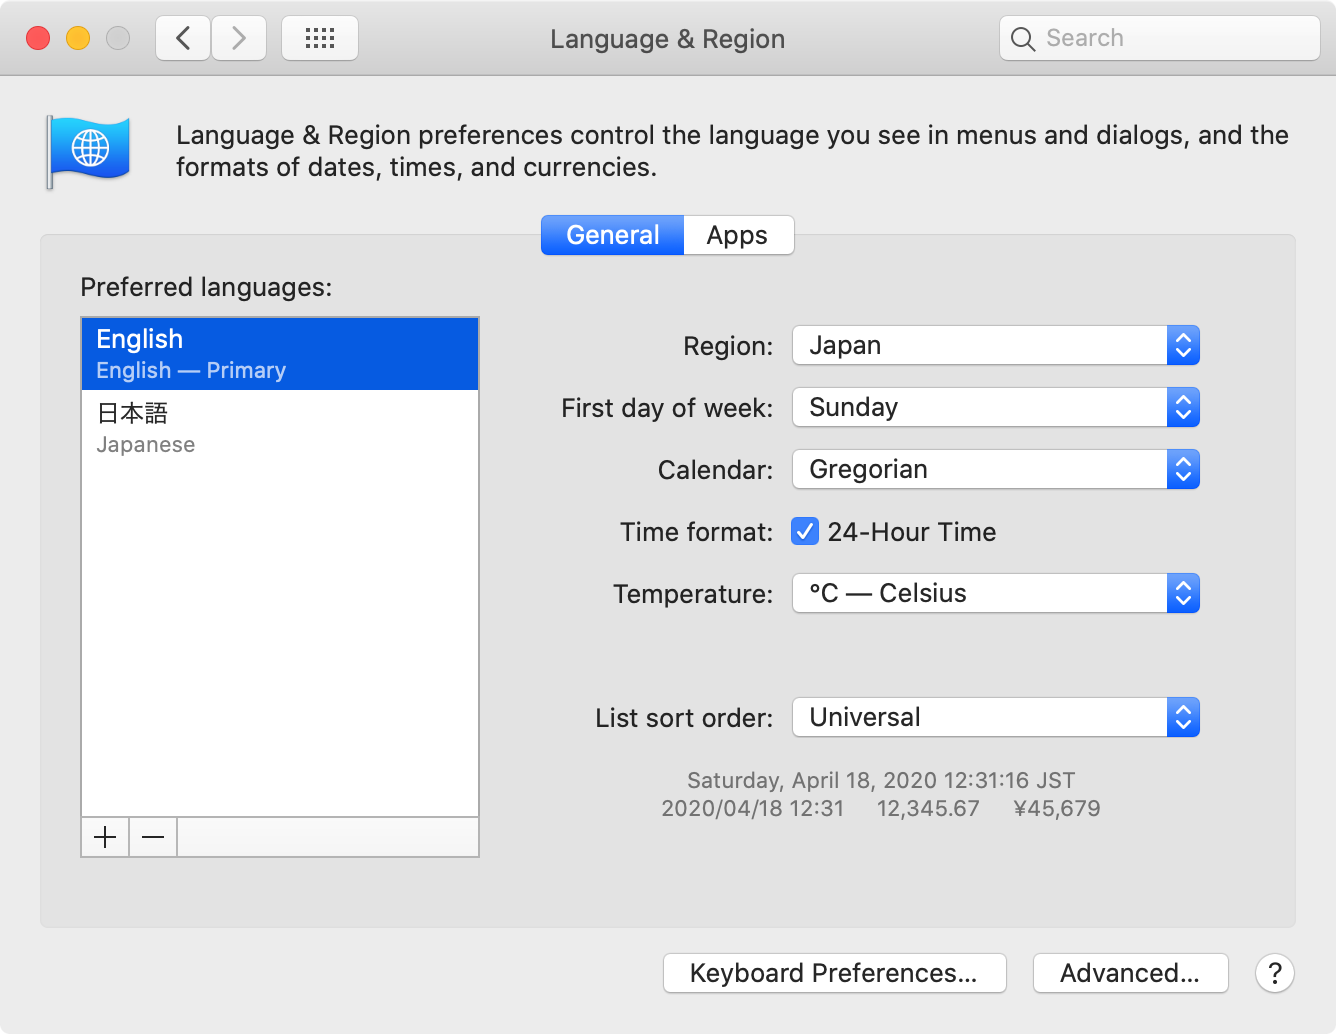
\includegraphics[scale=0.35]{fig/SystemPreferences_language.png}
  \caption{System PreferencesからLanuage \& Region(日本語環境だと「言語と地域」)を開いたところ}
  \label{fig:SystemPreferences_language}
\end{figure}

\section{日本語入力}

もし使用しているMacが既に英語環境になっており、日本語入力ができない状態の場合、図~\ref{fig:SystemPreferences_input}のようにSystem PreferencesからKeyboardを開き、「Input Sources」のところに「Japanese」を追加してください。

\begin{figure}
  \centering
  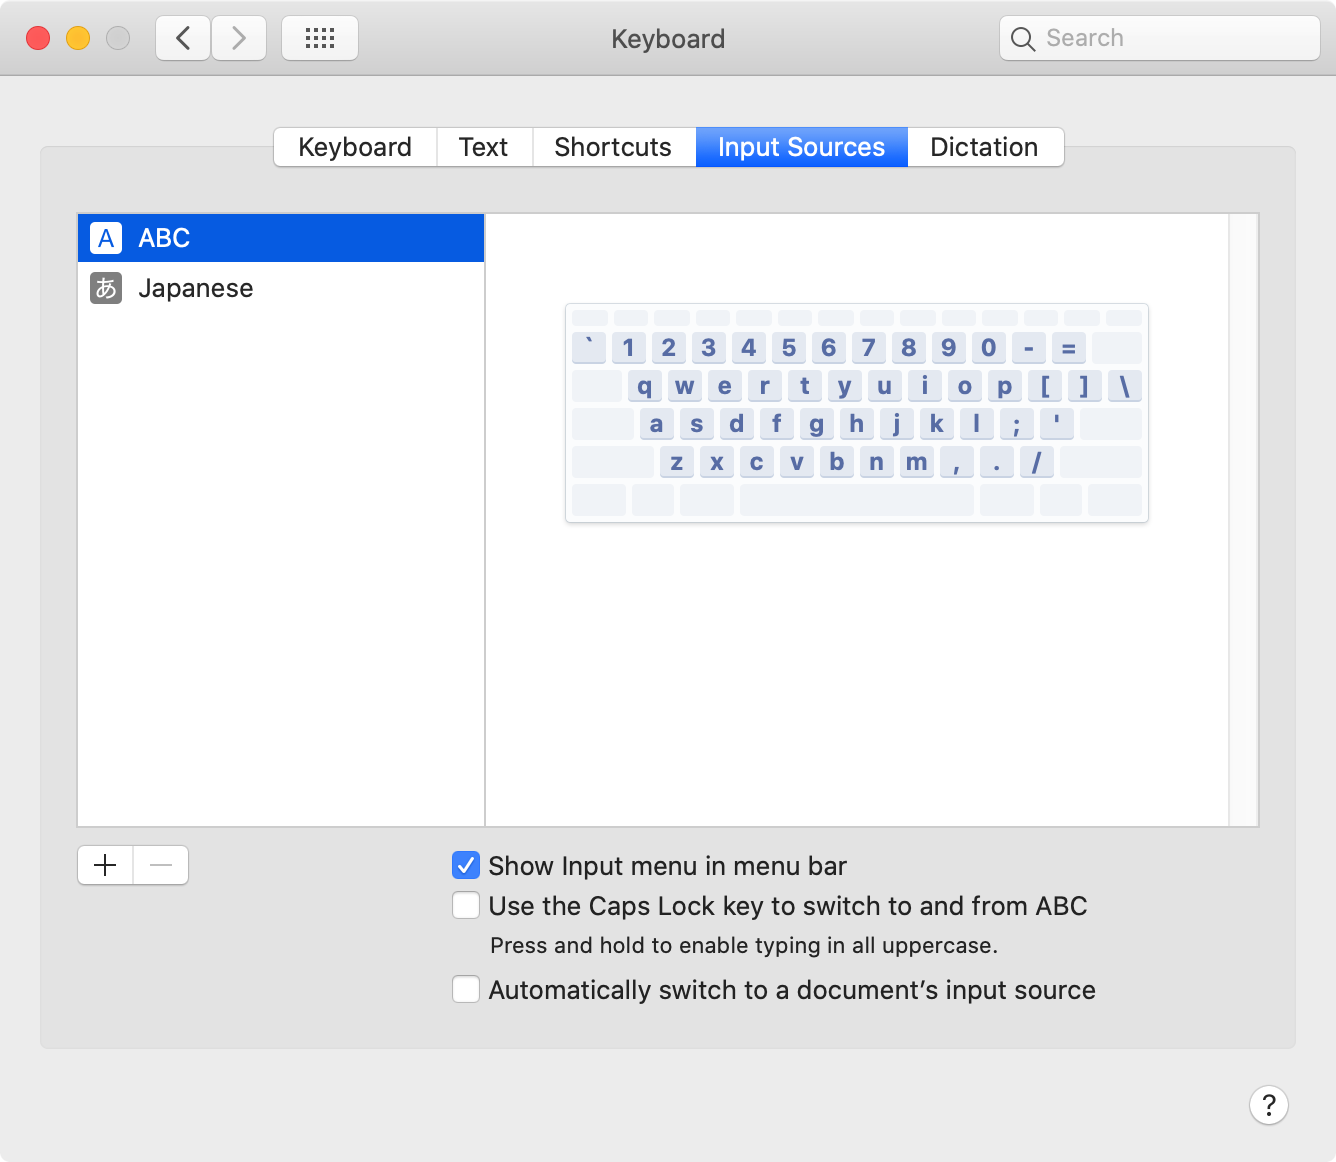
\includegraphics[scale=0.35]{fig/SystemPreferences_input.png}
  \caption{System PreferencesからKeyboardを開いたところ}
  \label{fig:SystemPreferences_input}
\end{figure}

日本語キーボード(JIS配列)のMacを使用している場合、スペースキーの左側に「英数」、右側に「かな」というキーがあるはずです。「英数」を押すと入力が英数に切り替わり、「かな」を押すと日本語入力(ローマ字入力)に切り替わります。もしUSキーボードを使用している場合、\ref{sec:Karabiner}節を参照し、左右のコマンドキーを「英数」と「かな」に割り当ててください。

日本語入力と英語入力を切り替えて使っていると、日本語入力モードのときに英単語を打ってしまったり、英語入力モードのときに日本語を打ってしまうという失敗をすることがあります。このような場合、入力済みの文字をいちいち消去する必要はありません。もし日本語入力モードで英単語を打ってしまったら、「英数」キーを左手の親指で2回素早く叩いてください。これで入力済みの文字がアルファベットに変換され、英語入力モードに切り替わります。逆に、英語入力モードのときに日本語を間違えて打ちかけた場合は、「かな」きーを右手の親指で2回叩いてください。

日本語入力と英語入力の切り替えは\ctlkey\,Spaceでも可能です。しかし、これは\ref{sec:Emacs}~節で後述するショートカットと競合してしまうため、節~\ref{sec:Keyboard}で設定を無効にします。

\section{Finderの設定}
まずはFinderの設定をしましょう。macOSのアプリケーションごと固有の設定は、それぞれのアプリケーションで「Preferences…」というメニューを選択することで行えます。Finderの場合、メニューバーのFinderからPreferences…を選びます。ショートカットは多くのアプリケーションで\cmdkey\,,です。

\begin{figure}
  \centering
  \subfigure[]{
    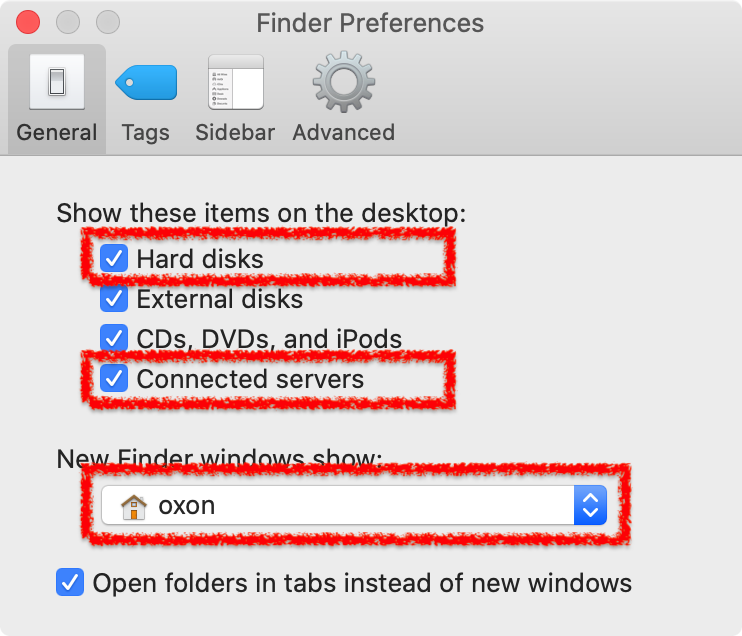
\includegraphics[width=.32\textwidth,clip]{fig/FinderPreferences_general.png}%
    \label{fig:FinderPreferences_general}%
  }\hfill%
  \subfigure[]{%
    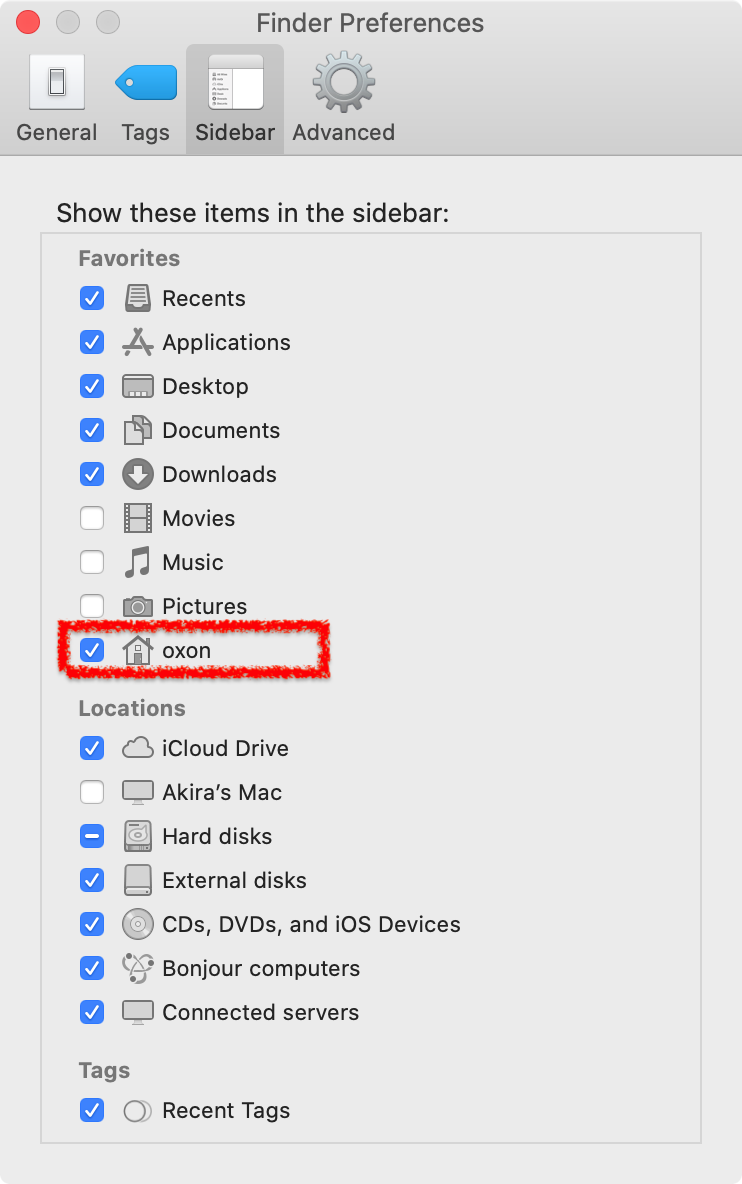
\includegraphics[width=.32\textwidth,clip]{fig/FinderPreferences_sidebar.png}%
    \label{fig:FinderPreferences_sidebar}%
  }\hfill%
  \subfigure[]{%
    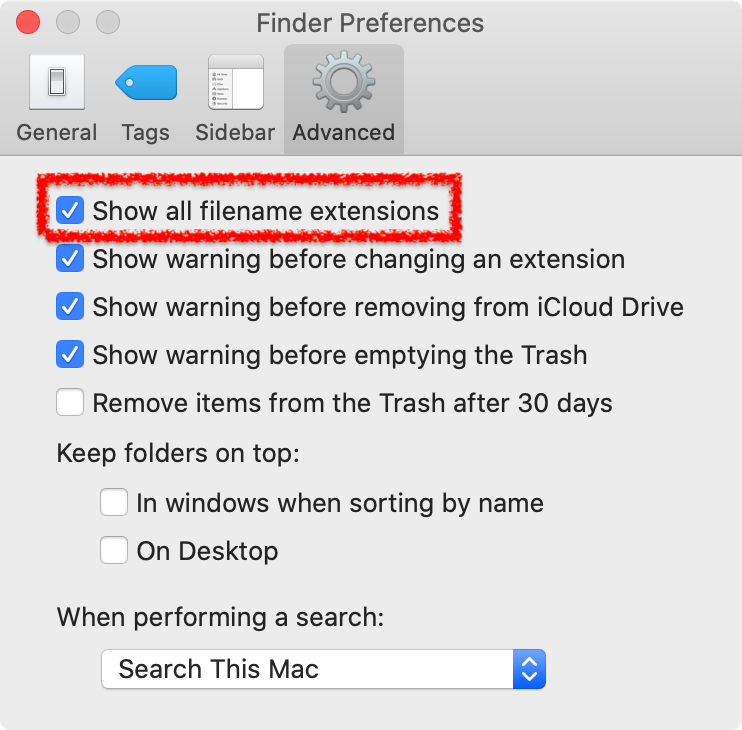
\includegraphics[width=.32\textwidth,clip]{fig/FinderPreferences_advanced.png}%
    \label{fig:FinderPreferences_advanced}
  }
  \caption{Finderの設定}
\label{fig:FinderPreferences}
\end{figure}

まずデスクトップに内蔵ハードディスク(SSD含む)と接続したサーバを表示するように、図~\ref{fig:FinderPreferences_general}を見て「General」のタブから設定を変更します。また新規にウィンドウを開いたときにホームが表示されるようにします。

次にSidebarのタブから図~\ref{fig:FinderPreferences_sidebar}のように表示する項目にホームを追加します。

最後に「Advanced」のタブを開きます。Macの初期設定では、ファイルの拡張子(extension)が表示されませんので、図~\ref{fig:FinderPreferences_general}のように全ての拡張子を表示する設定に変更します。この表示をしないと、Terminal.appから操作するファイル名とFinderから見えるファイル名が一致しない場合があります。

またディレクトリ階層がわかりやすいように、Finderがアクティブな状態で\cmdkey\,/と\cmdkey\,\optkey\,Pをそれぞれ押します。これで図~\ref{fig:Finder_info}のように項目数やパスの表示がされるようになります。

\begin{figure}
  \centering
  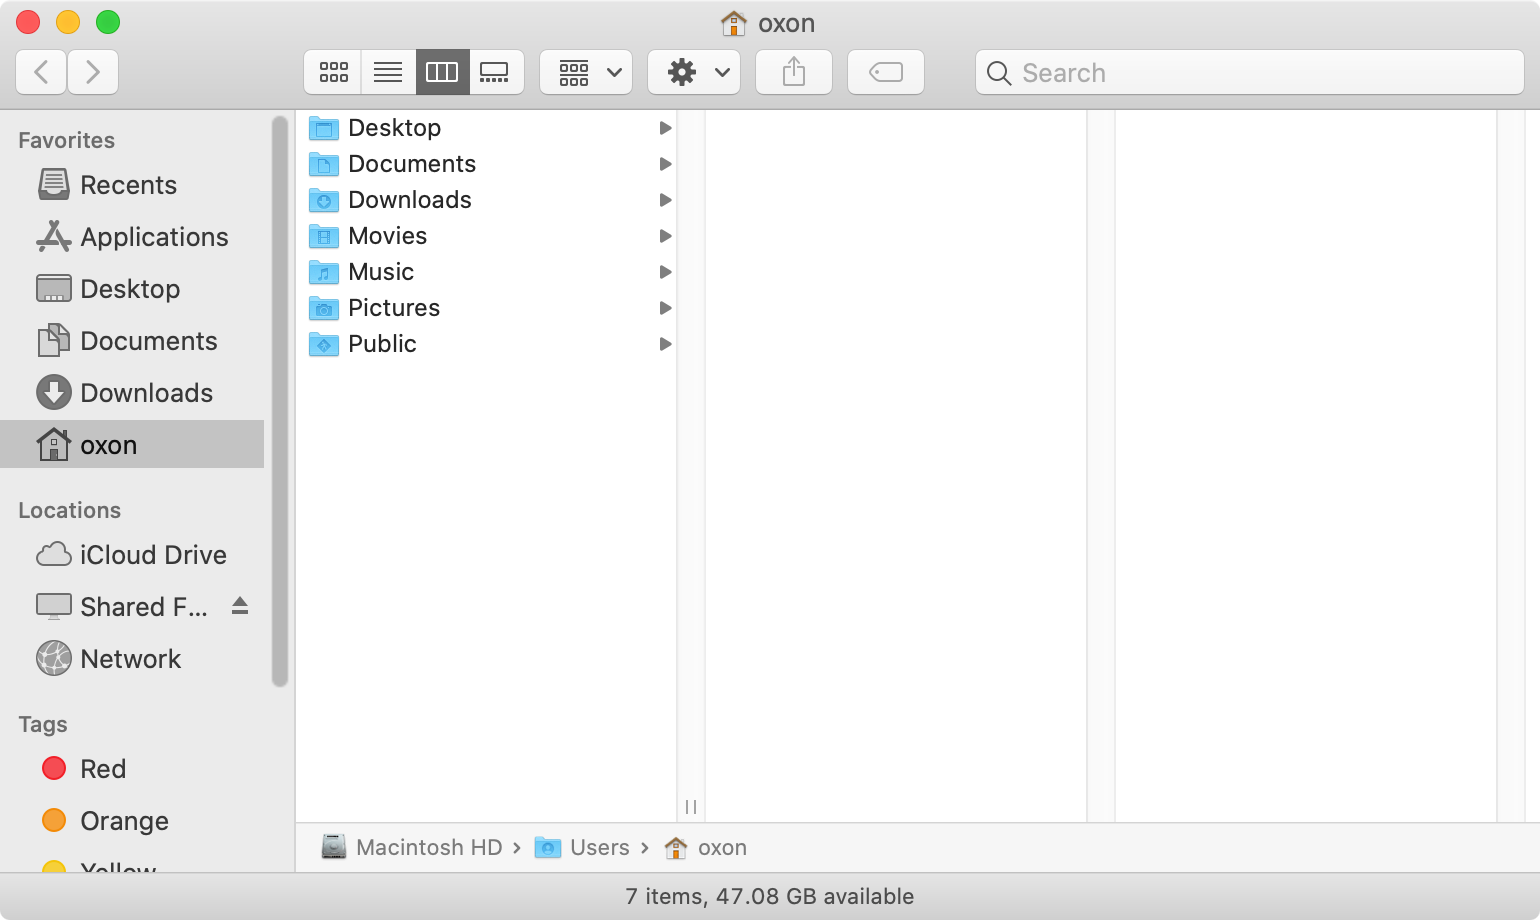
\includegraphics[width=.48\textwidth,clip]{fig/Finder_info.png}
  \caption{Finderの表示を変更した例}
\label{fig:Finder_info}
\end{figure}

\section{キーボードの設定}
\label{sec:Keyboard}

\subsection{Caps LockキーをControlキーに変更する}
もしあなたのMacがUS配列のキーボードならば、Caps LockキーはControlキーとして機能するように設定を変更しましょう。図\ref{fig:Keyboard1}のように、System Preferencesから「Keyboard」を開き「Modifier keys…」を押し、Caps LockをControlにします。\ref{sec:Emacs}~節で後述するように、macOS環境ではEmacsの操作体系に倣ったキーボードショートカットが使われています。そのためControlキーの使用率が他のOSに比べて非常に高くなるのが特徴です。US配列のキーボードを使用している場合にはControlキーが押しにくい位置にあるため、滅多に使わない、かつ最も押しやすい位置にあるCaps LockをControlキーにしてしまうことがよく行われています。

\begin{figure}
  \centering
  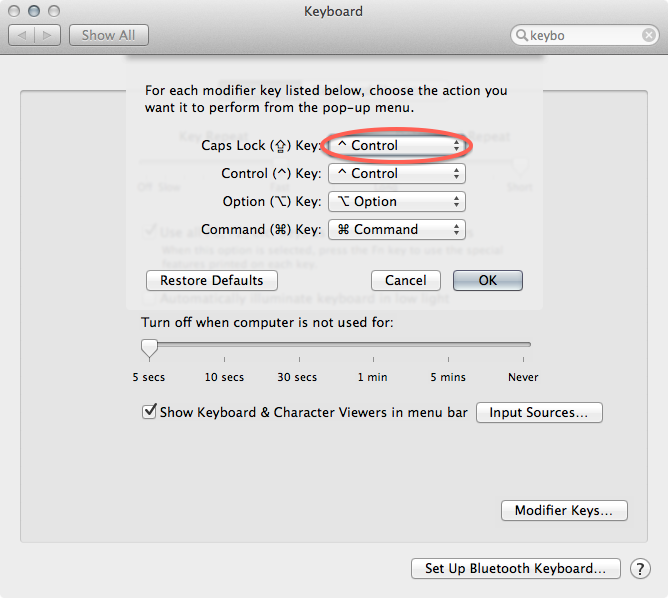
\includegraphics[scale=0.35]{fig/Keyboard1.png}
  \caption{Caps LockをControlキーに変更する}
  \label{fig:Keyboard1}
\end{figure}

\ref{sec:Karabiner}~節で説明するKarabiner-Elementsをインストールする場合、ここでのCaps Lockキーの置き換えはする必要はありません。Karabiner-Elementsで同様の設定を行います。

\subsection{入力切り替えの無効化}
日本語入力と英語入力の切り替えは、デフォルトでは\ctlkey\,Spaceになっています。しかしこれは図\ref{fig:Keyboard2}のように「Shortcuts」タブから無効化します。「英数」キーと「かな」キーから切り替えてください。

\begin{figure}
  \centering
  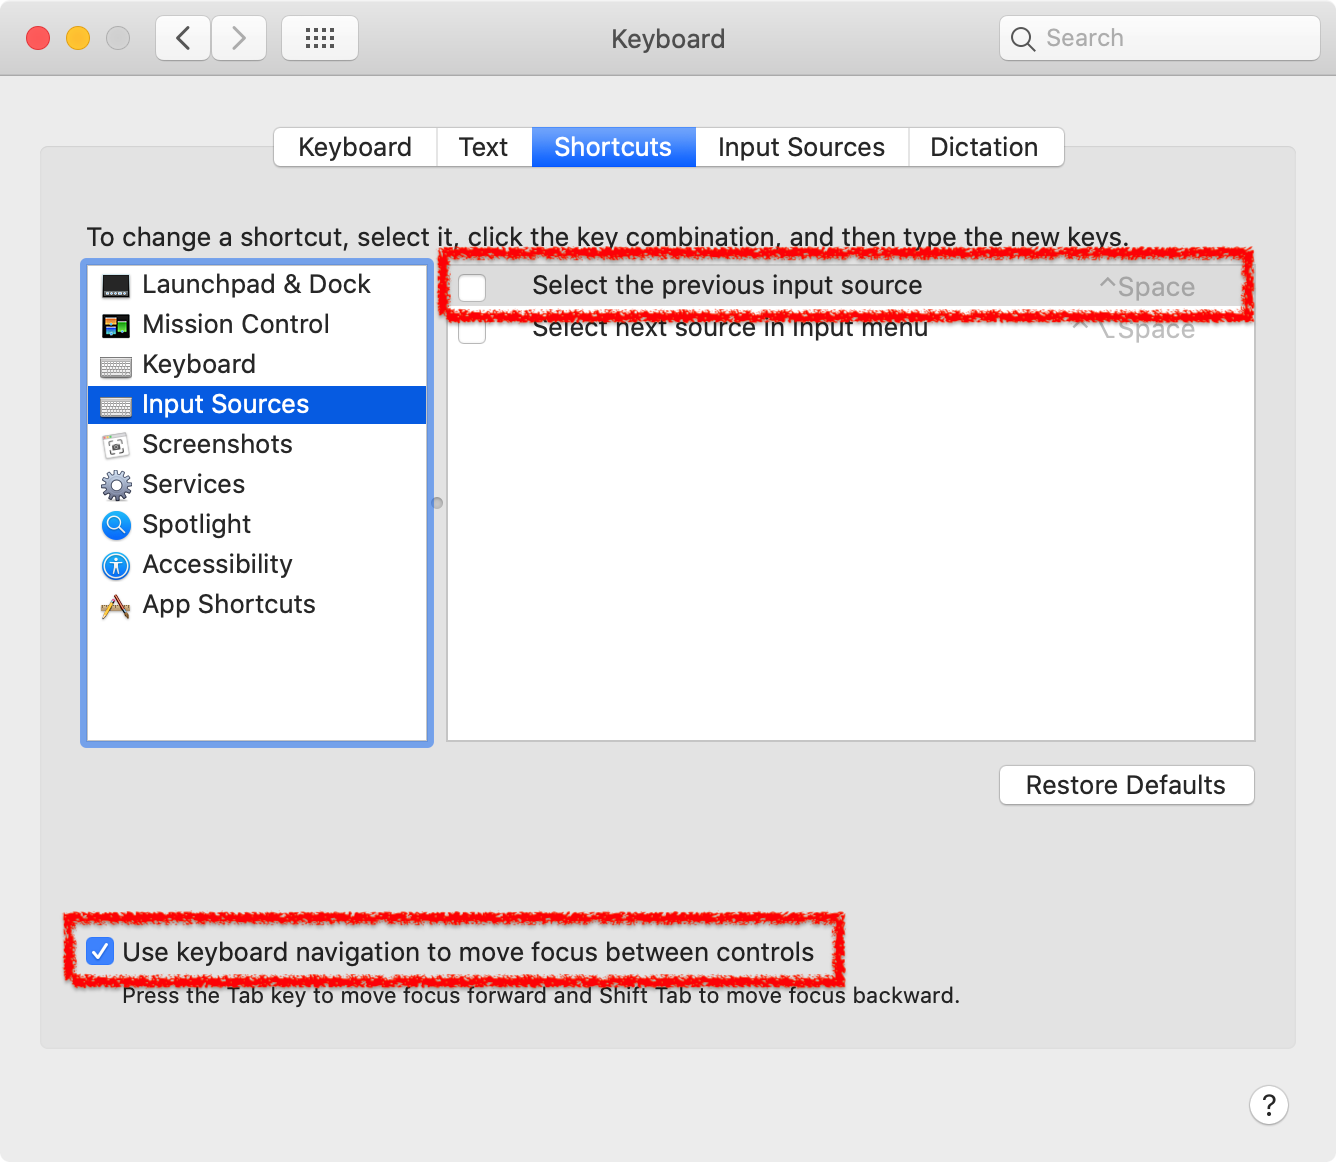
\includegraphics[scale=0.35]{fig/Keyboard2.png}
  \caption{入力の切り替えを無効化し、また全てのボタンなどをTabキーで移動できるようにする}
  \label{fig:Keyboard2}
\end{figure}

\subsection{Tabキーの動作の変更}
次に同じく「Shortcuts」のタブから、図\ref{fig:Keyboard2}のようにボタンなどの選択を全てTabキーで行えるようにします。このようにすることで、様々な画面操作をするときに、いちいちキーボードからトラックパッドやマウスへ手の移動をしなくて済むようになります。

例えばゴミ箱(Trash)を空にする際、図\ref{fig:Trash_Dialog}のような確認ダイアログが出てくるはずです。ここで数回Tabキーを押すと「Cancel」ボタンの強調表示(青線での縁取り)が「Empty Trash」との間で移動します。縁取られているボタンは、いちいちクリックしなくてもSpaceキーを押すと実行されます。また「Empty Trash」のように青く塗りつぶされているボタンは、リターンキーを押すと実行されます。

\begin{figure}
  \centering
  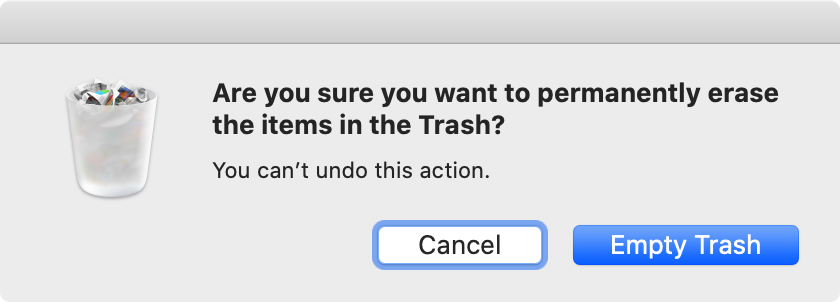
\includegraphics[scale=0.35]{fig/Trash_Dialog.png}
  \caption{ゴミ箱を空にするときのダイアログ}
  \label{fig:Trash_Dialog}
\end{figure}

\subsection{キーボードの繰り返し入力速度}
デフォルトでは、キーボードの繰り返し入力速度は非常に遅い設定になっています。例えばTerminal.appでaキーを押しっぱなしにしても、えらいのんびりと入力されます。図~\ref{fig:Keyboard_speed}のように、キーの繰り返し入力の速度を一番速くしてください。また繰り返し入力が開始されるまでの待ち時間も一番短くしてください。トラックパッド(Trackpad)のカーソル移動速度も、同じようにSystem Preferences のTrackpadのところから最速にしましょう。慣れてください。人生は時間が限られています。

\begin{figure}
  \centering
  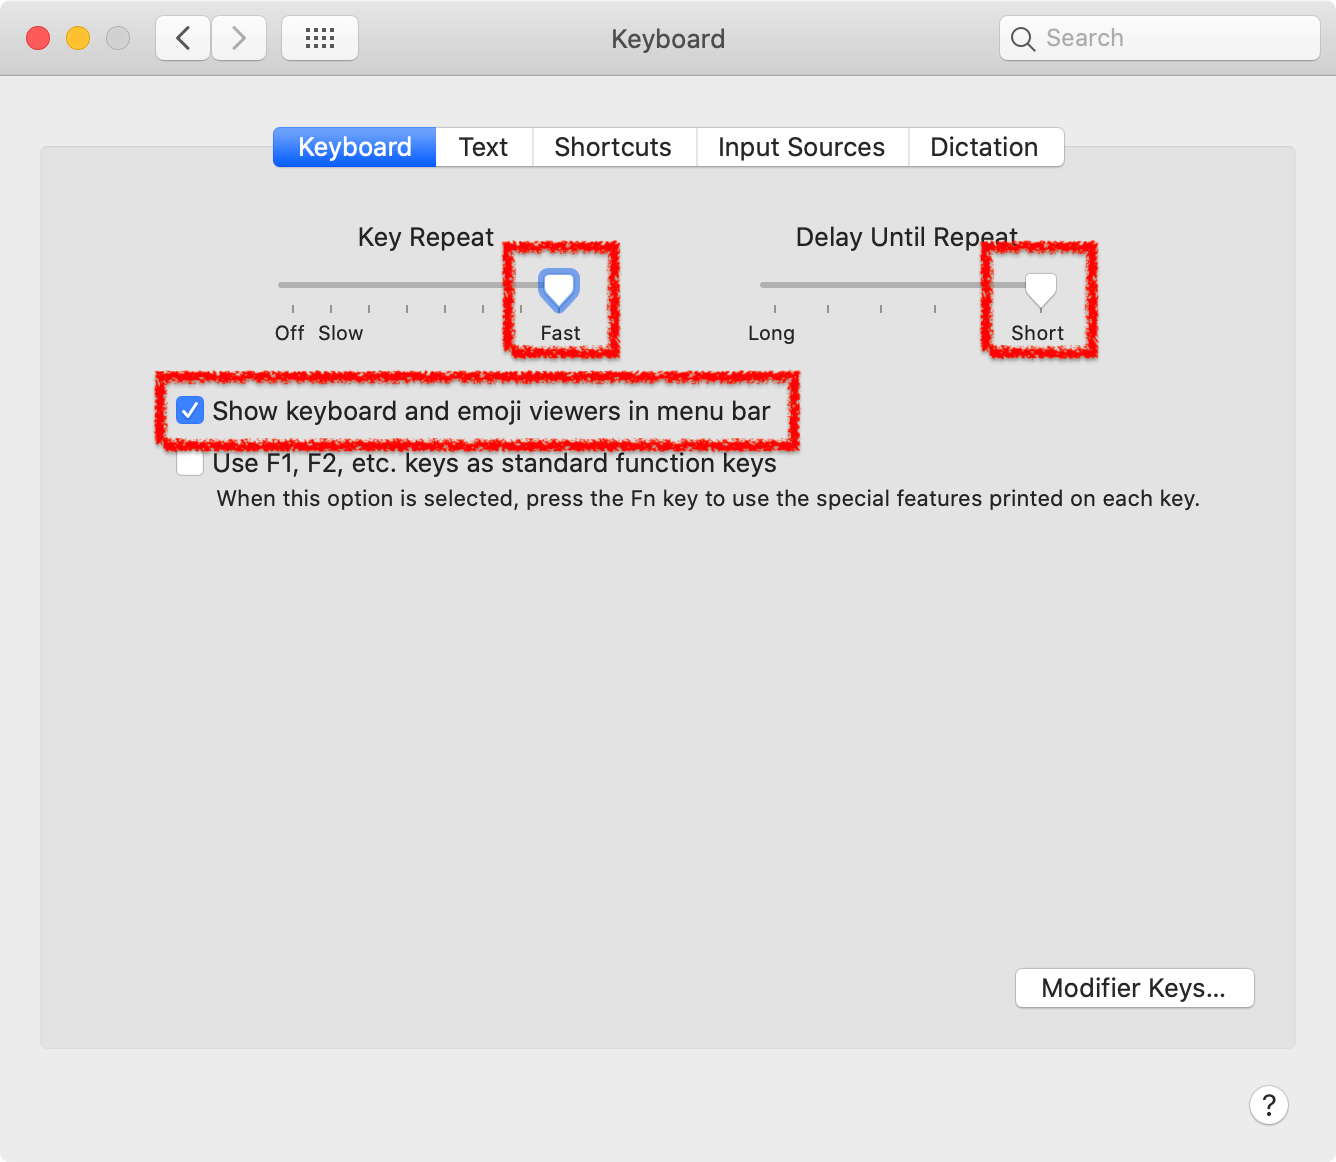
\includegraphics[scale=0.35]{fig/Keyboard_speed.png}
  \caption{繰り返し入力速度の変更}
  \label{fig:Keyboard_speed}
\end{figure}

ついでに、メニューバーの入力メニューのところから、記号や絵文字を探すパネルを表示できるようにしておくと便利です。

\section{Karabiner-Elementsによるキーボードの操作性向上}
\label{sec:Karabiner}

\ref{sec:Emacs}で述べるように、macOSのキーボード操作の多くはEmacsの操作体系に基づいています。しかし、この操作に対応していないアプリケーションも存在するため(Microsoft製品やAdobe製品など)、Karabiner-Elements\footnote{\url{https://karabiner-elements.pqrs.org}}をインストールすることでmacOSの操作を快適にすることができます。

他のmacOSアプリケーションのインストールでも同様の手順を踏むことがあるため、ここではKarabiner-Elementsを例として、インストール方法を簡単に説明します。

まずKarabiner-Elementsのウェブサイトから、ディスクイメージをダウンロードします\footnote{ディスクイメージ(disk image)とはmacOSのファイル形式のひとつで、マウント可能なボリューム(例えばUSBメモリなど)のように取り扱えるものです。拡張子は\texttt{.dmg}です。}。図~\ref{fig:Karabiner_download}のように、ダウンロードしたファイルはSafariのDownloadsの一覧に表示され、また\texttt{\~{}/Downloads}の中に保存されることが分かります。

\begin{figure}
  \centering
  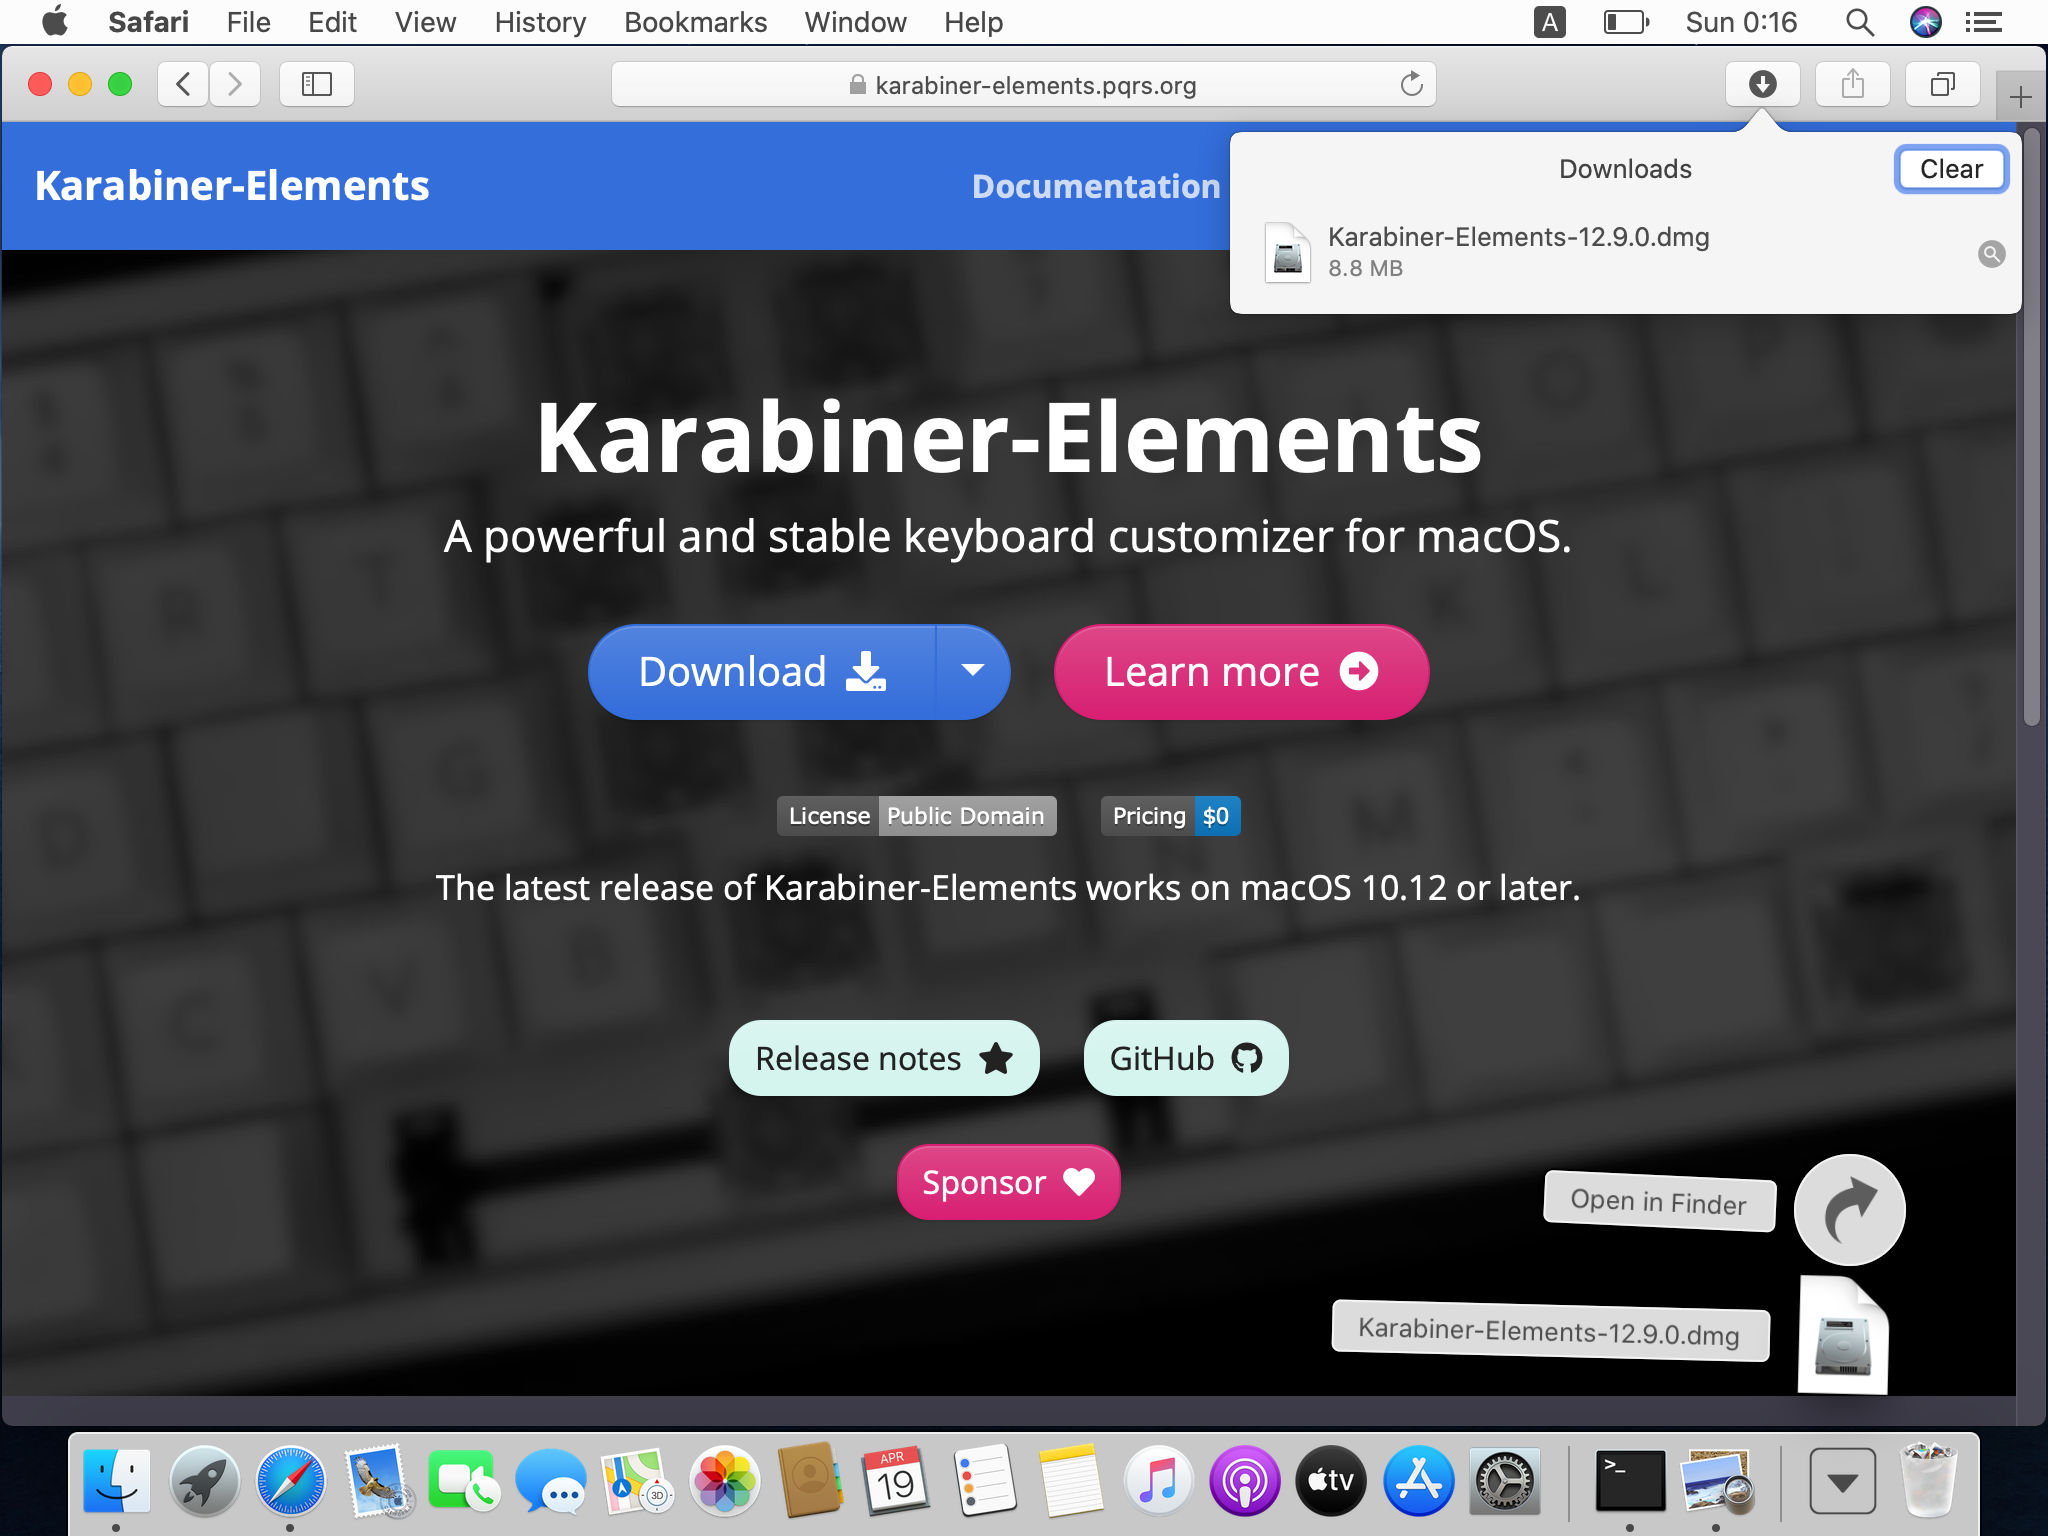
\includegraphics[scale=0.35]{fig/Karabiner_download.png}
  \caption{Karabiner-Elementsのダウンロード}
  \label{fig:Karabiner_download}
\end{figure}

このディスクイメージを開くと仮想的にマウントされ、デスクトップ上にマウント済みのボリュームが表示されます。この中に、パッケージファイル\footnote{パッケージファイル(package file)とは、macOSで複数のフォルダやファイルから構成されるものを擬似的に単一ファイルのように表示しているものです。拡張子は\texttt{.pkg}です。}が図~\ref{fig:Karabiner_pkg}のように存在します。これがインストーラーです。

\begin{figure}
  \centering
  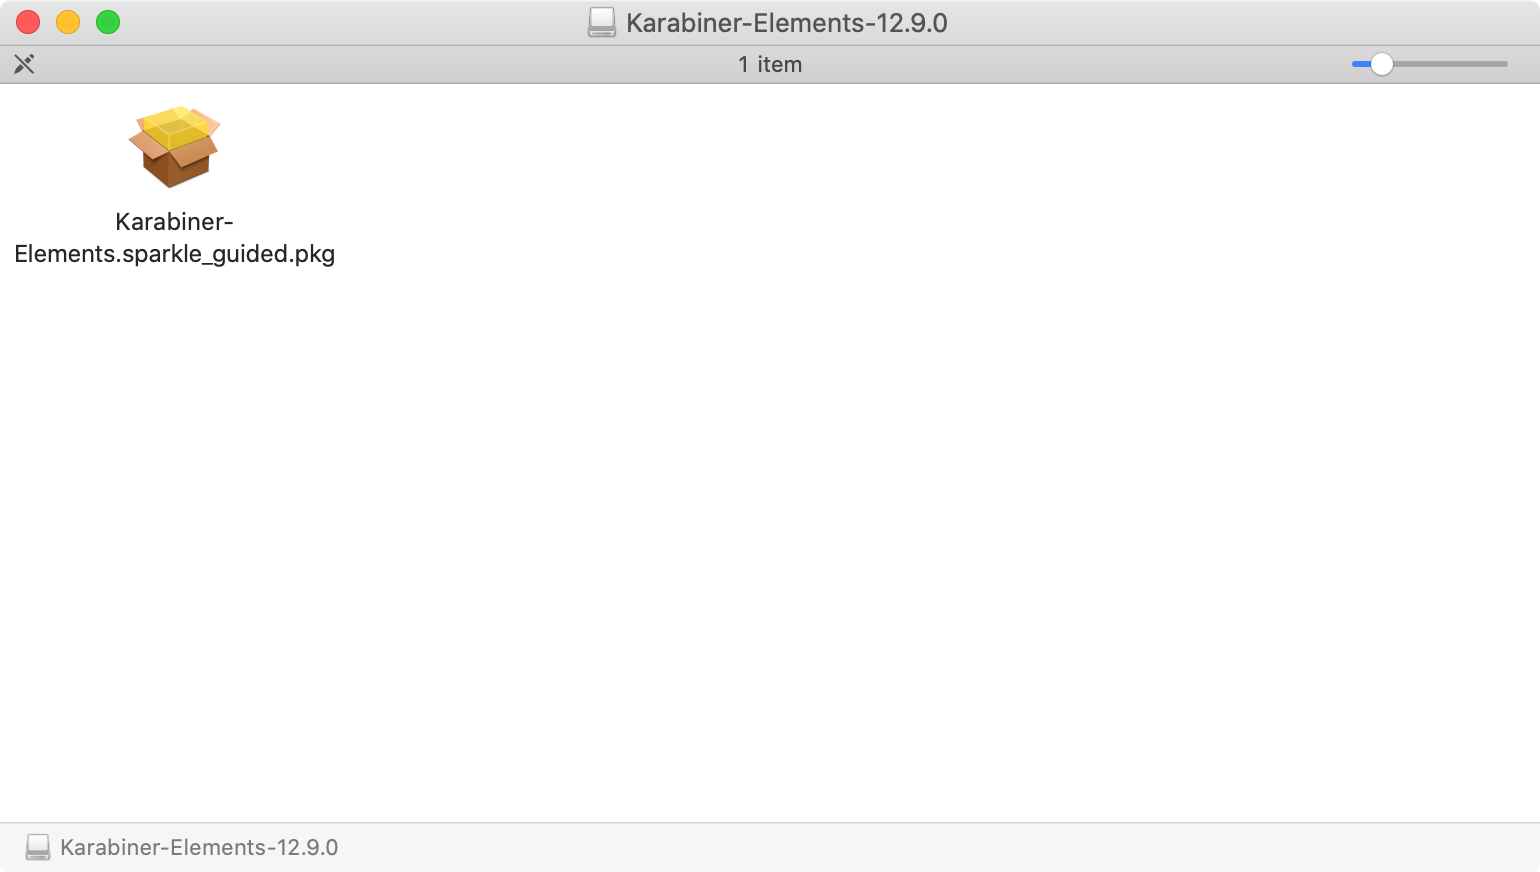
\includegraphics[scale=0.35]{fig/Karabiner_pkg.png}
  \caption{Karabiner-Elementsのインストールパッケージ}
  \label{fig:Karabiner_pkg}
\end{figure}

インストーラーを起動すると、図~\ref{fig:Karabiner_install}のようにmacOSの標準的なインストール画面が表示されます。表示される手順にしたがってインストールしてください。公式の説明は\url{https://karabiner-elements.pqrs.org/docs/getting-started/installation/}にあります。

\begin{figure}
  \centering
  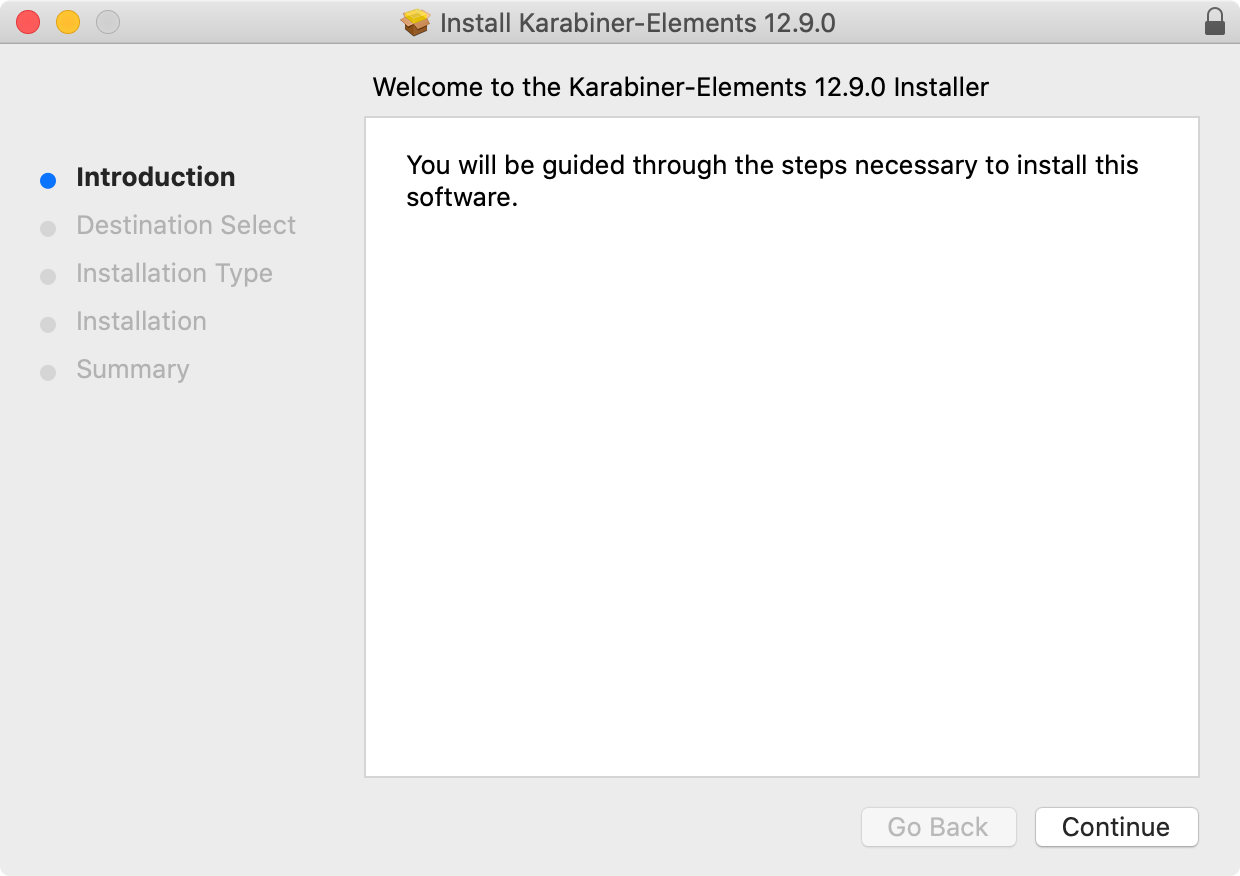
\includegraphics[scale=0.35]{fig/Karabiner_install.png}
  \caption{Karabiner-Elementsのインストール画面}
  \label{fig:Karabiner_install}
\end{figure}

このインストールを進めると、図~\ref{fig:Karabiner_blocked}のような警告が表示されます。これは、App Storeなどの認証を経ていないソフトウェアをインストールしたり起動したりする場合などに表示されます。コンピュータウイルスのように悪意の持ったプログラムを実行するときもこのような警告が出るはずですので、インストールしようとしているにはソフトウェアが怪しいものでないか、よく注意してください。

\begin{figure}
  \centering
  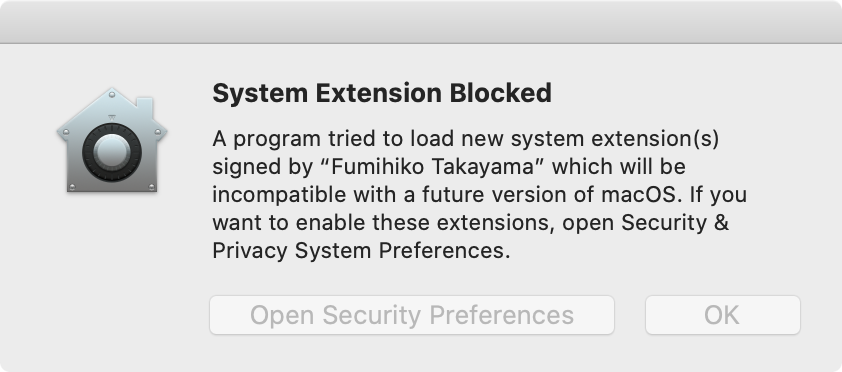
\includegraphics[scale=0.35]{fig/Karabiner_blocked.png}
  \caption{Karabiner-Elementsの警告}
  \label{fig:Karabiner_blocked}
\end{figure}

この警告ではインストールしようとしている機能拡張(System Extension)がブロックされたと書かれています。これを解除するためには、指示に従い、System Preferences の Security \& Privacy を開いてください。

そうすると、図~\ref{fig:Karabiner_allow}のような画面になっているはずです。まず左下の鍵アイコンをクリックして管理者権限で解錠します。このように管理者権限が必要となるOSの設定変更は、この鍵アイコンをその都度クリックする必要があります。解錠するとブロックされたソフトウェアを許可するためのAllowボタンが押せるようになります。今回の場合、Karabiner-Elementsとその開発者である Fuihiko Takayama 氏は信頼できますので、Allowを押してください。これで、Karabiner-Elementsのインストール作業は終わりです。

\begin{figure}
  \centering
  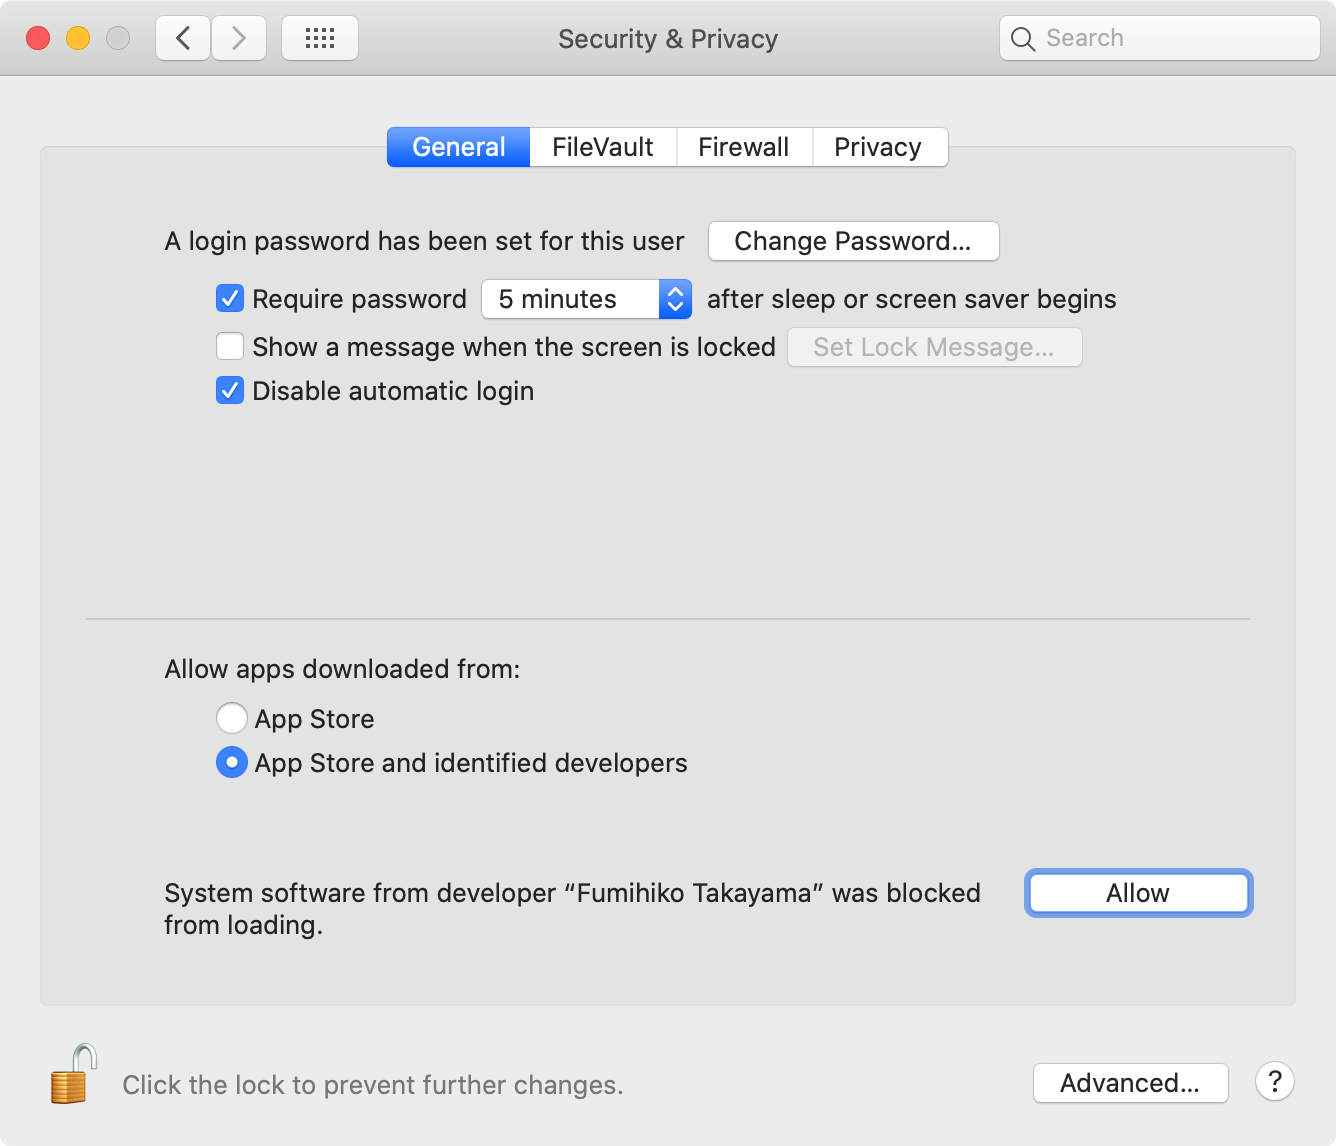
\includegraphics[scale=0.35]{fig/Karabiner_allow.png}
  \caption{Karabiner-Elementsの許可}
  \label{fig:Karabiner_allow}
\end{figure}

Karabiner-Elementsをインストール後、SpotlightからKarabiner-Elements.appを起動してください。そうすると、まず最初に図~\ref{fig:Karabiner_keystroke}のように許可を求めるダイアログが出るはずです。このようなダイアログは、一部のアプリケーションの初回起動時に現れることが頻繁にあります。Karabiner-Elementsの場合はキーボード入力を受け取り特殊な処理を行うため、そのような動作に対してユーザの許可が必要となるからです。また例えばZoomでは画面共有をする機能がありますが、これもセキュリティ上の問題が潜在的にあるため、ユーザの許可を必要とし、同様のダイアログが表示されます。

\begin{figure}
  \centering
  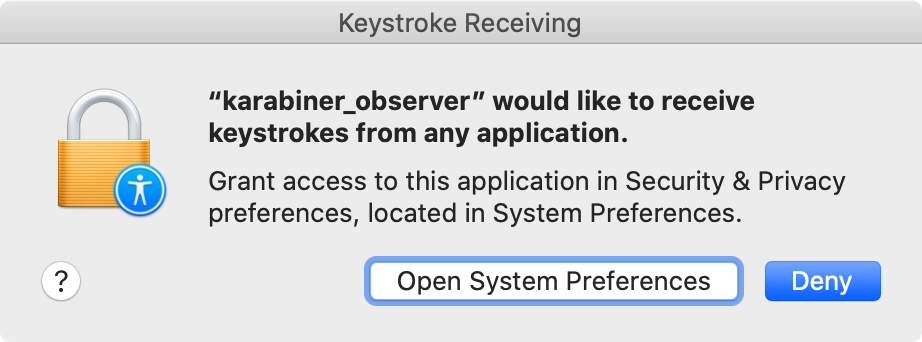
\includegraphics[scale=0.35]{fig/Karabiner_keystroke.png}
  \caption{Karabiner-Elementsのキーボード入力への警告}
  \label{fig:Karabiner_keystroke}
\end{figure}

このダイアログに従い「Open System Preferences」をクリックすると、図~\ref{fig:Karabiner_privacy}が現れます。ここで再び鍵アイコンを解錠し、Karabiner-Elements関係のファイルがキーボード入力を読み取れるように許可を出します。

\begin{figure}
  \centering
  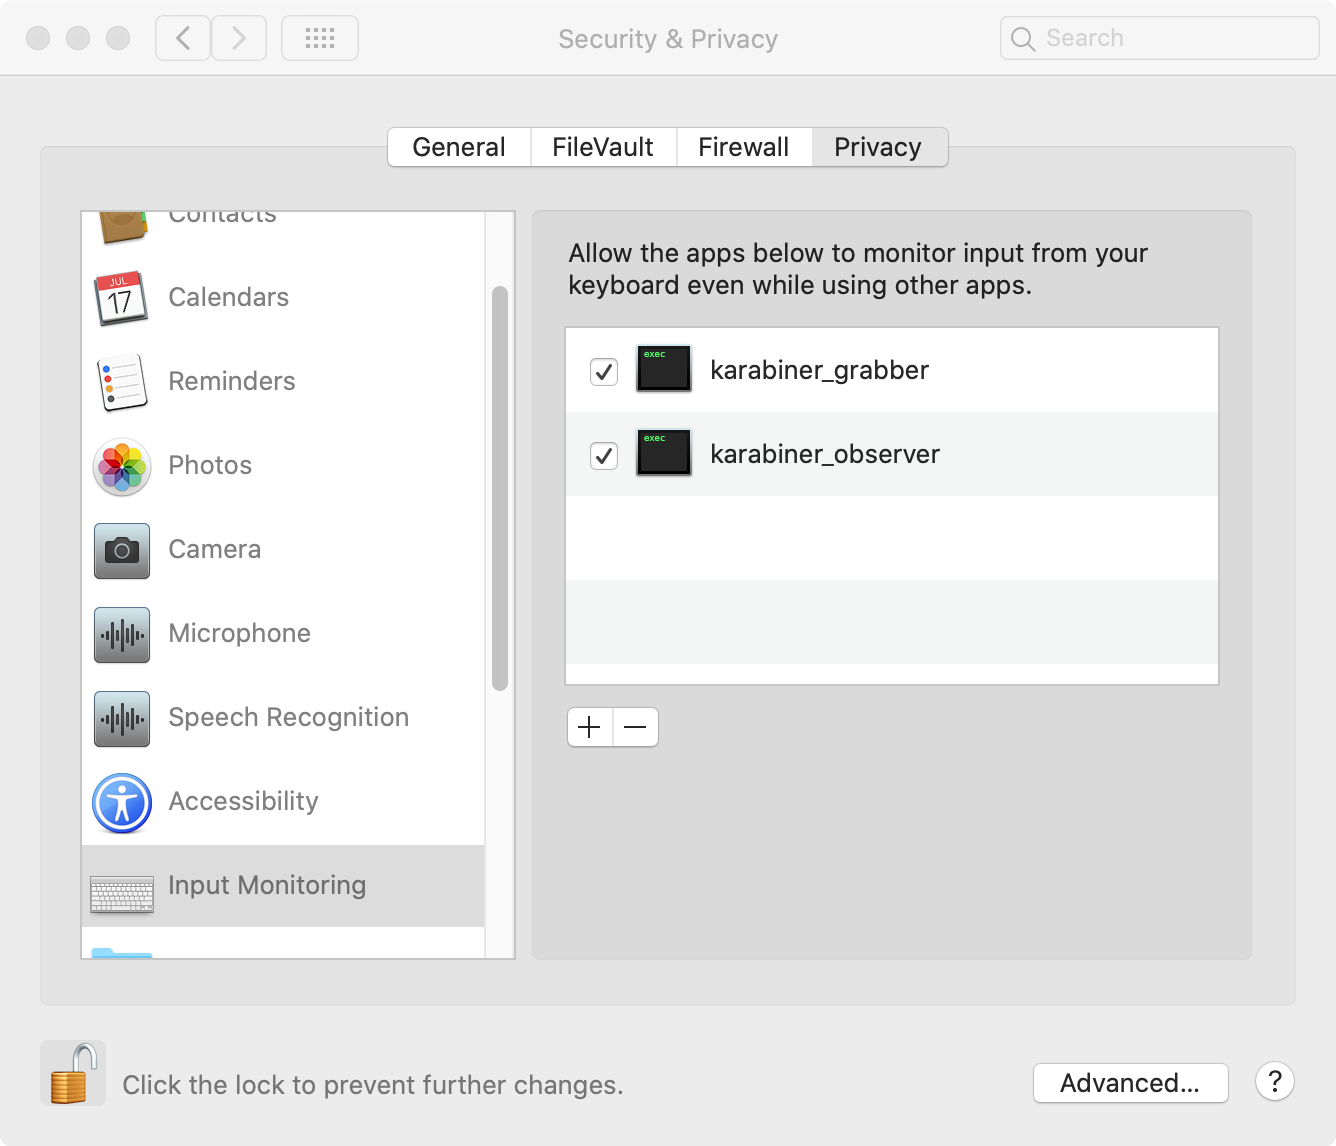
\includegraphics[scale=0.35]{fig/Karabiner_privacy.png}
  \caption{Karabiner-Elementsのプライバシー設定}
  \label{fig:Karabiner_privacy}
\end{figure}

さて、これでようやくKarabiner-Elementsが使用できます。USキーボードを使用している場合は、まず図~\ref{fig:Karabiner_simple}のように「Simple modifications」のタブでCaps LockキーをControlキーに変更してください。

\begin{figure}
  \centering
  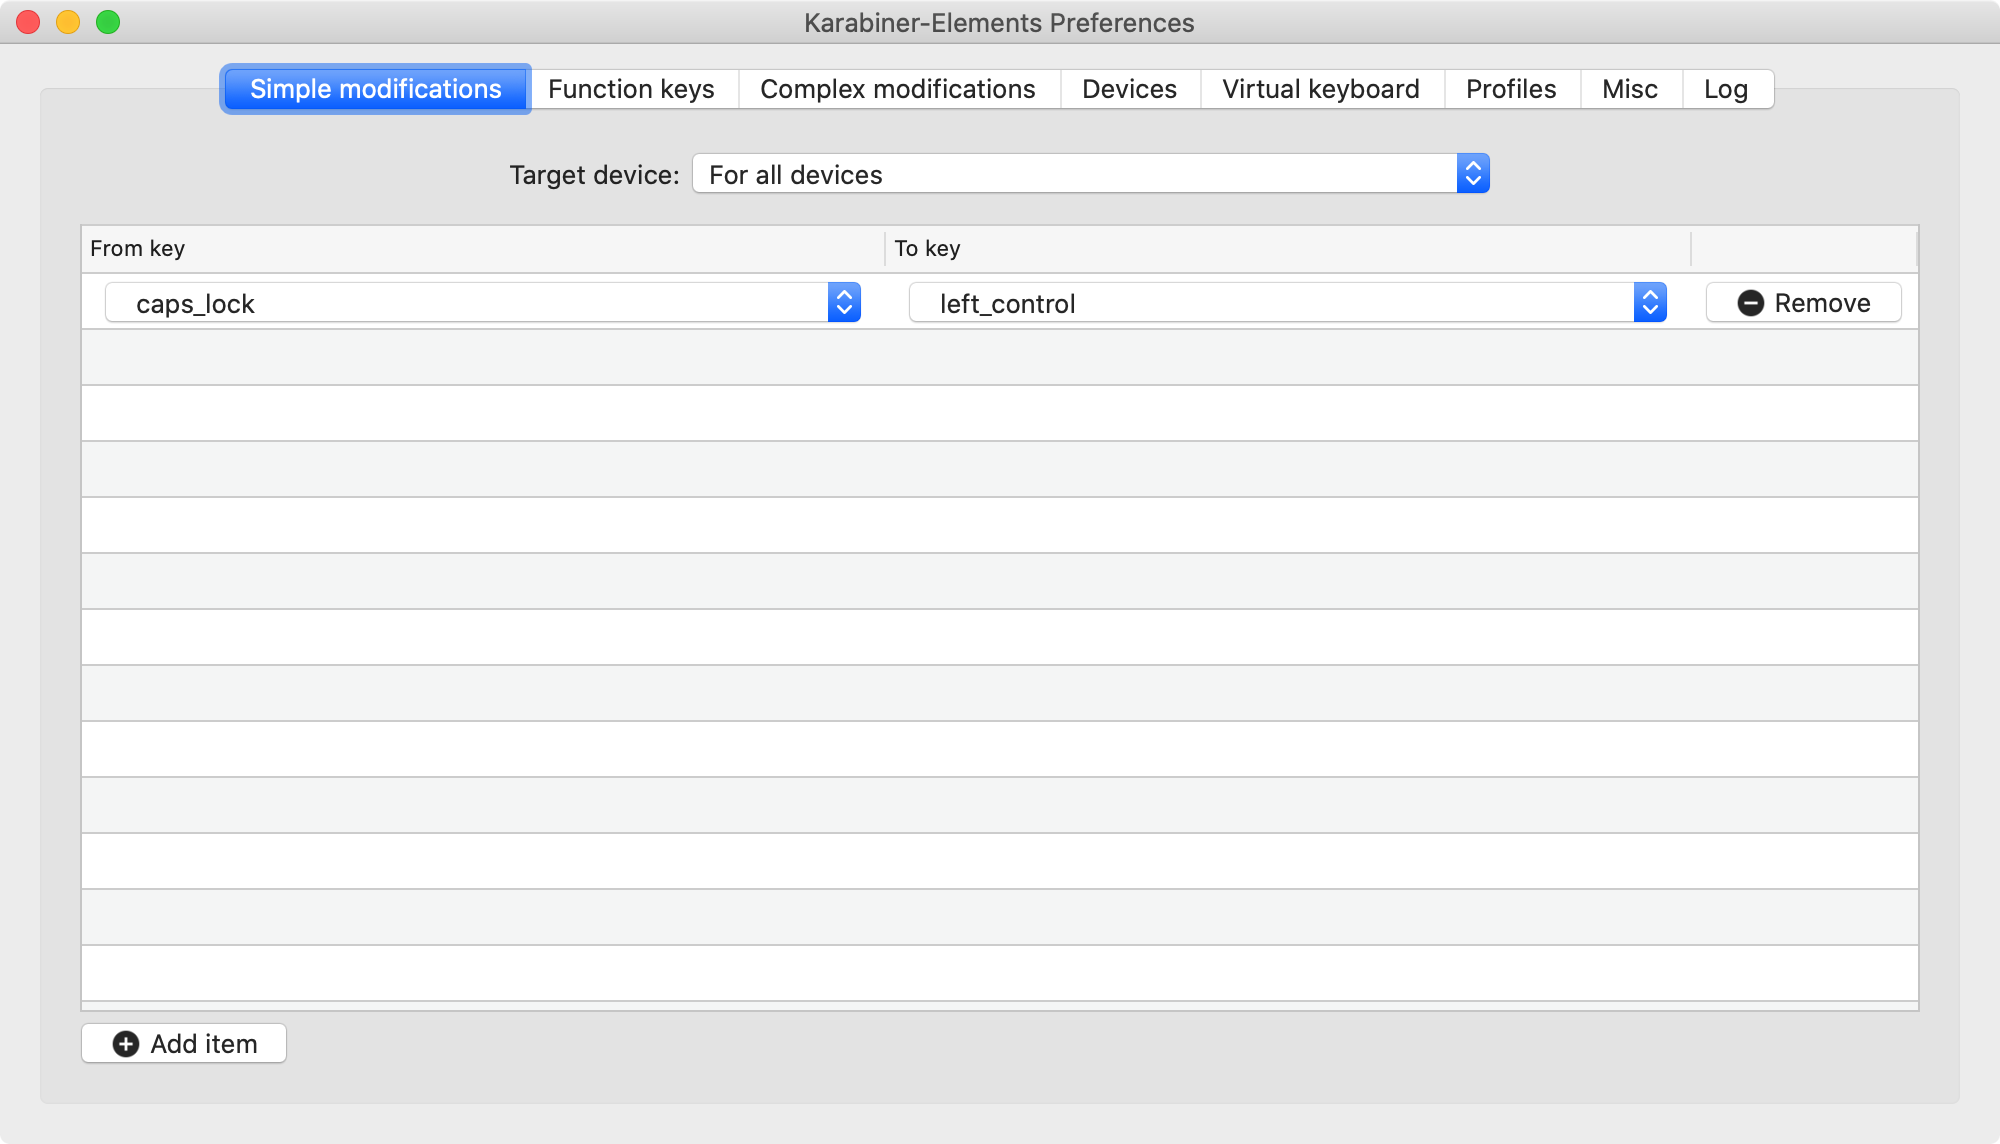
\includegraphics[scale=0.35]{fig/Karabiner_simple.png}
  \caption{Karabiner-Elementsの設定画面}
  \label{fig:Karabiner_simple}
\end{figure}

次に図~\ref{fig:Karabiner_import}のように「Complex modifications」タブから「Add rule」クリックし、「Import more rules from the Internet」を押してください。様々なキーボード動作の設定がダウンロードできるので、「Emacs key bindings (rev 12)」をダウンロードしましょう。USキーボードの場合は「For Japanese (日本語環境向けの設定) (rev 5)」も追加します。

\begin{figure}
  \centering
  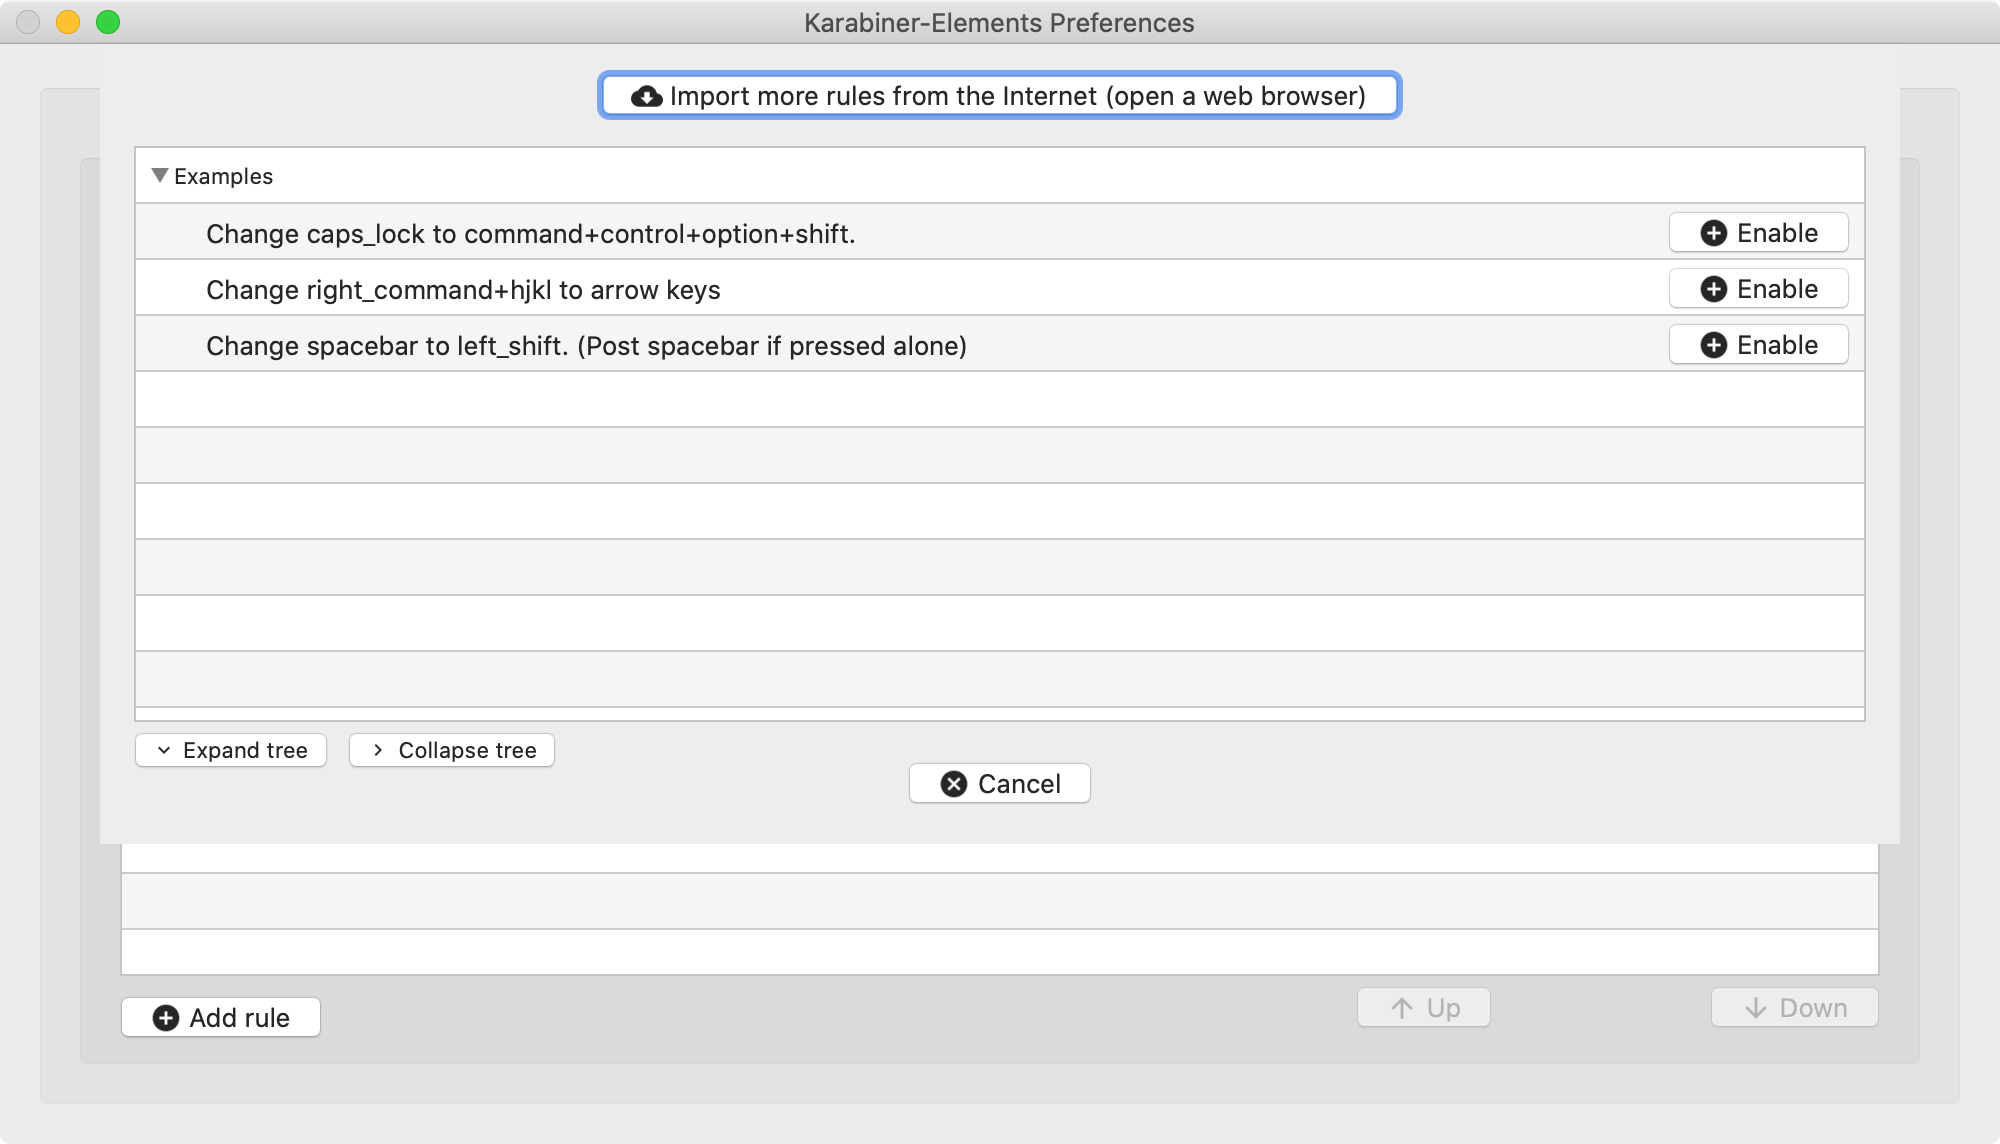
\includegraphics[scale=0.35]{fig/Karabiner_import.png}
  \caption{Karabiner-Elementsの設定のインポート}
  \label{fig:Karabiner_import}
\end{figure}

最後に「Emacs key bindings [control+keys] (rev 10)」を「Enable」にします。USキーボードの場合は「コマンドキーを単体で押したときに、英数・かなキーを送信する。(左コマンドキーは英数、右コマンドキーはかな) (rev 3)」も追加します。

\section{Emacsの操作体系に慣れる}
\label{sec:Emacs}

ここでは、macOSでの標準的なエディタ(editor)のひとつであるEmacsの操作について、その初歩の初歩について説明します\footnote{macOS Mojaveまでは\texttt{/usr/bin/emacs}が最初からインストールされていましたが、Catalinaからはなくなりました。GNUライセンスで配布されているソフトウェアの使用を回避するためと言われています。代わりに\texttt{/usr/bin/mg}というEmacsに似たエディタ(Emacsクローン)がインストールされています。}。エディタは文章を書くためのソフトウェアです。ただし、ワープロのように様々な装飾をするための機能はありません。プログラムを書いたり、\LaTeX{}のソースを書いたりと、装飾ではなく文そのものに意味があるときに使います。そのような作業に特化したワープロにはない様々な機能が搭載されています。

Emacsの特徴のひとつに、文字入力に特殊なキーボードショートカット(Emacs key binding)を使うことが挙げられます。慣れないうちは全く便利に感じないと思いますが、一度慣れてしまうと、もう他のエディタには戻れなくなるのでぜひ覚えて下さい。macOSを使う場合、このショートカットをほとんどのソフトウェアでも利用可能です。基本的なキーボードショートカットの一覧を表\ref{tab_emacs}にまとめました。

\begin{table}
  \centering
  \caption{Emacsの基本的なキーボードショートカット}
  \label{tab_emacs}
  \begin{tabular}{llp{10cm}}
  \hline
ショートカット & 英単語 & 機能 \\ \hline\hline
C-f & {\bf F}orward & 一文字進む(→キーと同等) \\
C-b & {\bf B}ackward & 一文字戻る(←キーと同等) \\
C-p & {\bf P}revious line & 次の行へ進む(↓キーと同等) \\
C-n & {\bf N}ext line & 前の行へ戻る(↑キーと同等) \\
C-a & {\bf A}head & 行頭へ移動 \\
C-e & {\bf E}nd & 行末へ移動 \\
C-k & {\bf K}ill & カーソル位置から行末までを全て kill-ring と呼ばれるメモリ領域に移動(カットに類似) \\
C-y & {\bf Y}ank & kill-ringにあるものをカーソル位置にペースト \\
C-t & {\bf T}ranspose & カーソルの前後の文字を入れ替える \\
C-h & 不明 & カーソル前方を一文字削除(MacのDelete、WindowsのBackspaceと同等) \\
C-d & forward {\bf D}elete & カーソル後方を一文字削除(WindowsのDeleteと同等) \\
C-m & 不明 & 改行(カーソルも次の行へ移動する) \\
C-o & 不明 & 改行(カーソルは元の位置にとどまる) \\
C-Space C-w & 不明 & C-Space入力時のカーソル位置から、C-w入力時のカーソル位置までの範囲をkill-ringに移動する \\ \hline
C-x C-f & {\bf F}ind file & 既存ファイルを開く、なければ作成する \\
C-x C-s & {\bf S}ave & ファイルを保存する \\
C-x C-c & 不明 & 終了する \\
C-x C-w & 不明 & ファイルを別名で保存する \\
C-x C-2 & 不明 & ウインドウを二分割にする \\
C-x C-1 & 不明 & ウインドウを一分割にする \\
C-s & {\bf S}earch & 検索する \\
C-r & {\bf R}verse search & 後方に検索する \\
M gg & 不明 & 特定の行に移動する\\\hline
  \end{tabular}
\end{table}

\ref{sec:Homebrew}章を参考にして、まずはEmacsをインストールしてみてください。\texttt{Emacs}というコマンドを設定し終えたところまでを想定します。

次のコマンドで、Emacsを立ち上げます。図~\ref{fig:Emacs}のような画面が現れるはずです。
\begin{lstlisting}[language=bash]
$ Emacs
\end{lstlisting}

\begin{figure}
  \centering
  \subfigure[]{
    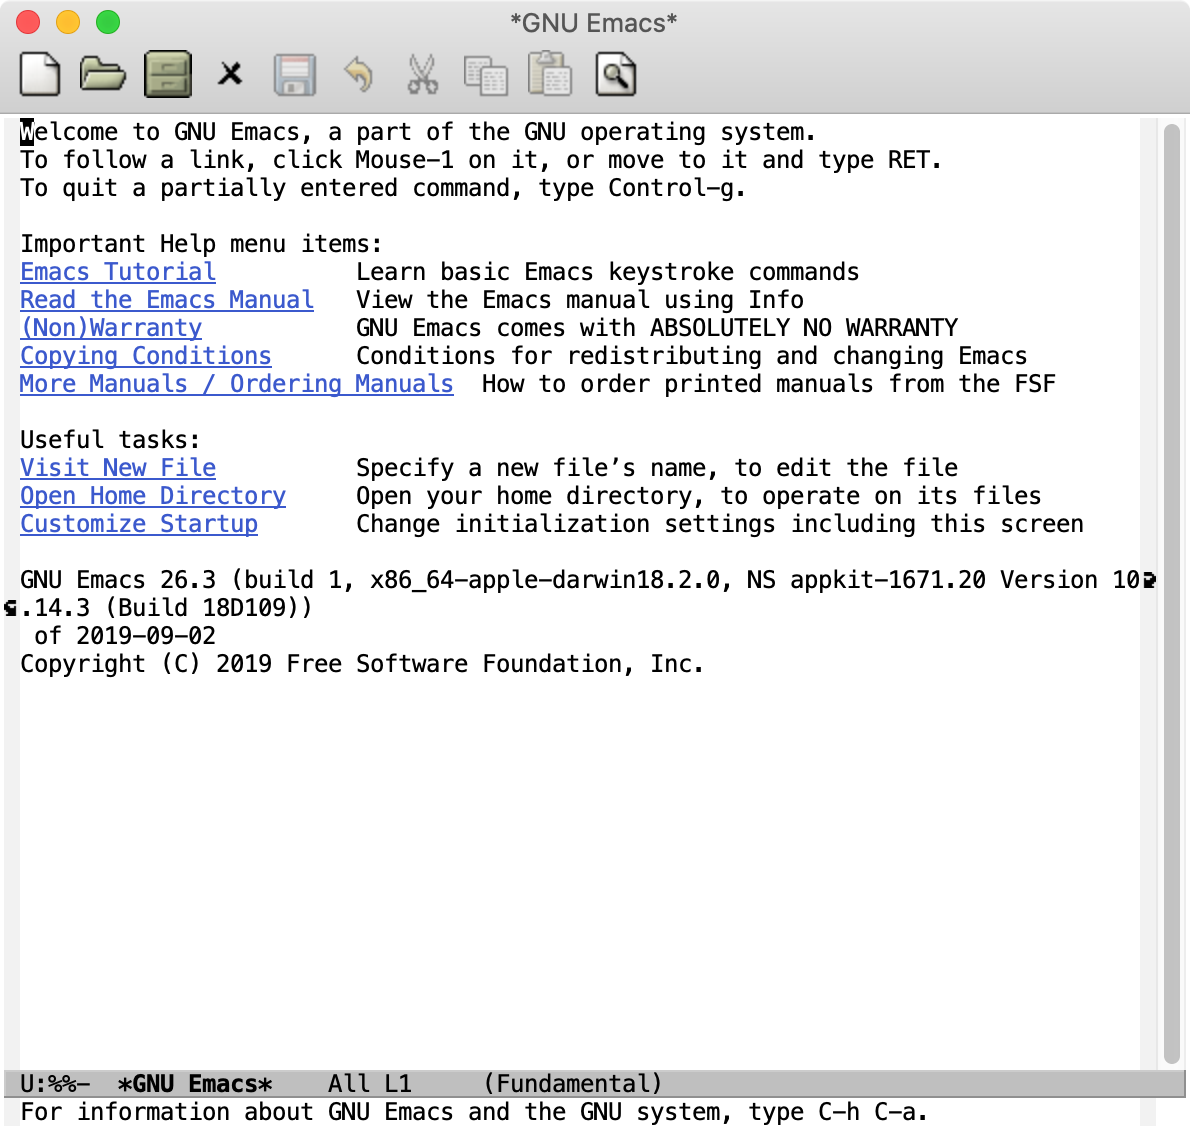
\includegraphics[width=.32\textwidth,clip]{fig/Emacs.png}%
    \label{fig:Emacs}%
  }\hfill%
  \subfigure[]{%
    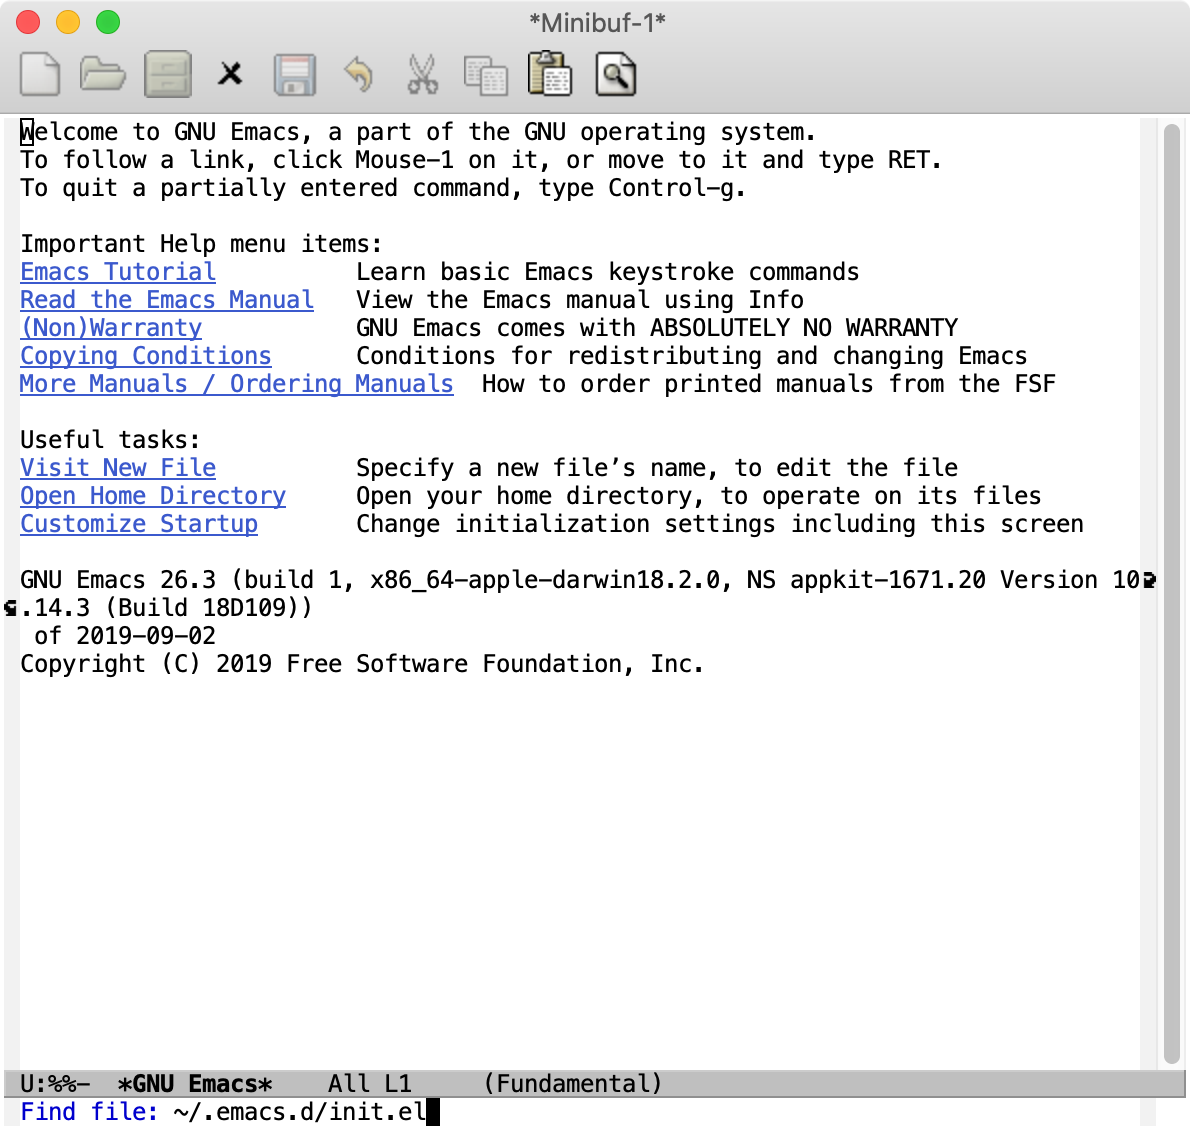
\includegraphics[width=.32\textwidth,clip]{fig/Emacs_CxCf.png}%
    \label{fig:Emacs_CxCf}%
  }\hfill%
  \subfigure[]{%
    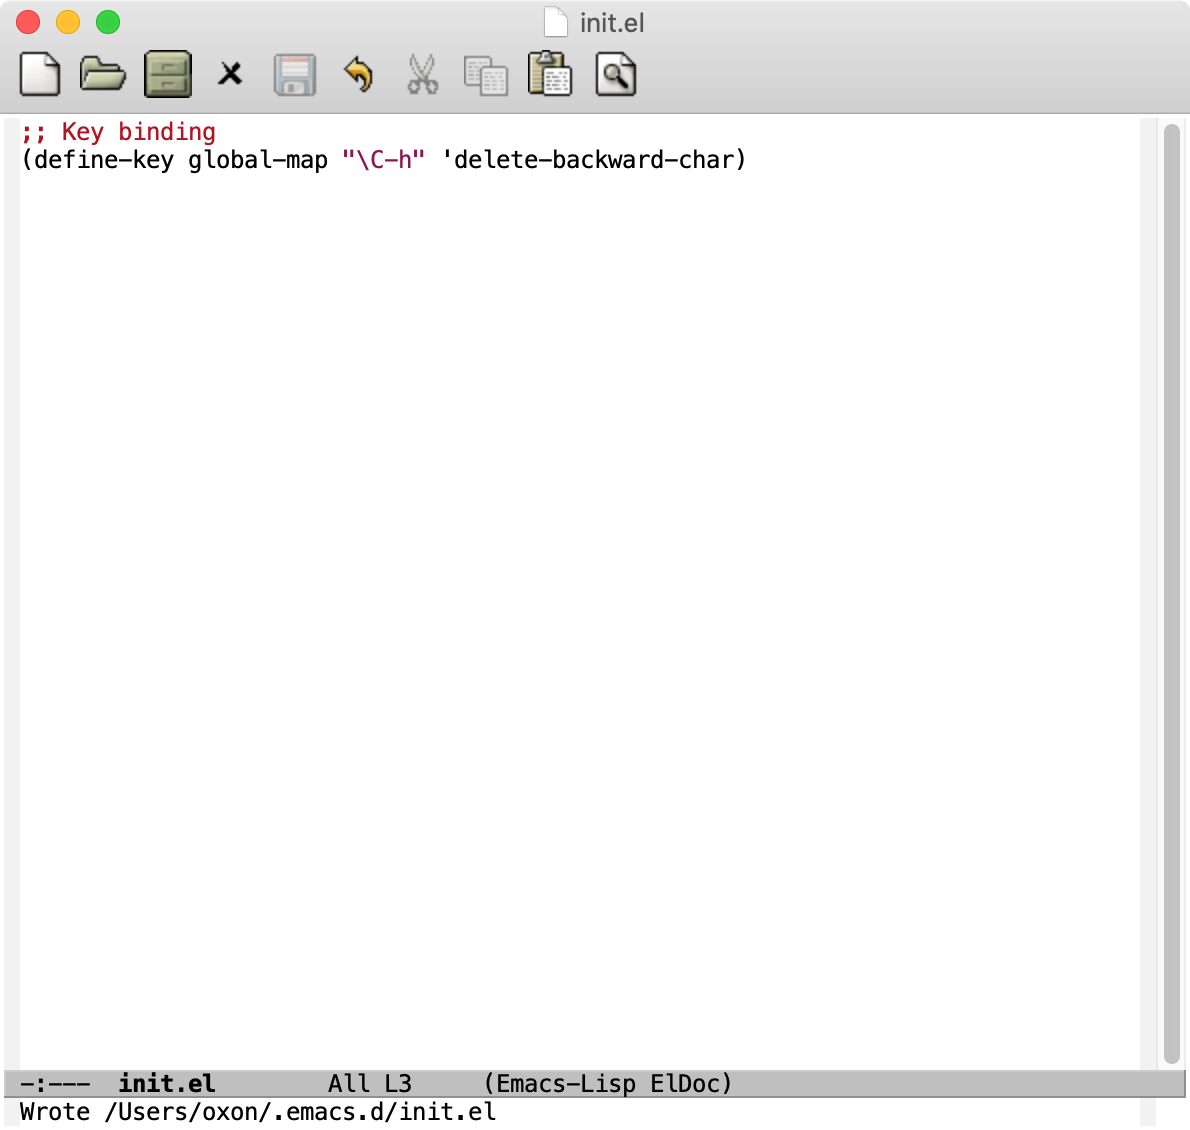
\includegraphics[width=.32\textwidth,clip]{fig/Emacs_CxCs.png}%
    \label{fig:Emacs_CxCs}
  }
  \caption{Emacsの起動画面 (a) Emacsを立ち上げたところ。(b) \texttt{C-x C-f}で\texttt{\~{}/.emacs.d/init.el}を新規作成するところ。(c) 編集後に\texttt{C-x C-s}で保存したときの画面。}
\end{figure}

まずは、新しいファイルを作成してみましょう。最初に作成するのは、Emacsの設定ファイルです。図~\ref{fig:Emacs}の状態から、Controlキー\footnote{USキーボードでCaps LockキーをControlキーに変更した場合は、そのキー。}を左手小指で押しっぱなしにし、左手中指でXキーを同時に押します。その後Xキーから薬指を離し、Controlキーは押した状態のまま左手人さし指でFキーを同時に押します。これを、「C-x C-f」のように表記します\footnote{Control-x、Ctl-x、Cn-xなど、いくつかの表記方法があります。好みの問題です。}。表\ref{tab_emacs}にあるように、これは新規ファイルを作成するためのショートカットです。図\ref{fig:Emacs_CxCf}のように一番下の「Find file:」の後に続けて作成したいファイル名を入力し、リターンきーを押しましょう。ここでは\texttt{\~{}/.emacs.d/init.el}を作成しています\footnote{これは、ホームディレクトリの中にある不可視ディレクトリ\texttt{.emacs.d}の中にある\texttt{init.el}というファイルの意味です。}。

そのファイルが存在しない場合は、新規作成されます。真っ白な画面に切り替わったら、次の内容を入力します。
\begin{lstlisting}[language=lisp]
;; Key binding
(define-key global-map "\C-h" 'delete-backward-char)
\end{lstlisting}
そして、\texttt{C-x C-s}で編集内容を保存すると、図~\ref{fig:Emacs_CxCs}のようになるはずです。最後に、\texttt{C-x C-c}でEmacsを終了します。ここで追加した設定は、1行目はただのコメント(なくても動作は変わりません)、2行目は\texttt{C-h}を1文字削除の動作に変更するための設定です。

Emacsの操作に慣れるには、まずこのControlキーを多用した操作に慣れることが重要です。表\ref{tab_emacs}に挙げたショートカットを中心にまずは覚え、どのような操作や機能、設定があるのかを調べていきましょう。多機能過ぎて、うんざりするはずです。

\section{C-Space C-wをmacOSで使う}

表\ref{tab_emacs}に示したショートカットの多くはmacOSのアプリケーションでも使うことができます。また使えないアプリケーションでも、\ref{sec:Karabiner}に書いたようにKarabiner-Elementsの設定で使用可能になります。

例えばKarabiner-Elementsで\texttt{C-p}や\texttt{C-f}を有効にしておくと、Finderのカラム表示での移動が非常に早く、楽になります。

しかしmacOSのデフォルトの状態では\texttt{C-Space C-w}はmacOSのアプリケーションでは使うことができません。Emacsに慣れてくると、\texttt{C-Space C-w}がEmacs以外で使えないのが不便に感じるでしょう。macOSにはこの操作を実現するための機能が隠されています。

コード\ref{code:DefaultKeyBinding}を、\texttt{\~{}/Library/KeyBindings/DefaultKeyBinding.dict}として保存して下さい\footnote{\url{https://developer.apple.com/library/archive/documentation/Cocoa/Conceptual/EventOverview/TextDefaultsBindings/TextDefaultsBindings.html}に詳しい解説がある。}。「Mail」などを起動して文字入力する際に、\texttt{C-Space C-w}や\texttt{C-x C-s}が有効になっているはずです。

%\begin{NoFloat}
\lstinputlisting[float=tb,caption=\texttt{DefaultKeyBinding.dict},label=code:DefaultKeyBinding,numbers=left]{src/DefaultKeyBinding.dict}
%\end{NoFloat}

\section{Xcode}

\begin{lstlisting}[language=bash]
$ clang
xcode-select: note: no developer tools were found at '/Applications/Xcode.app', requesting install. Choose an option in the dialog to download the command line developer tools.
\end{lstlisting}

\begin{figure}
  \centering
  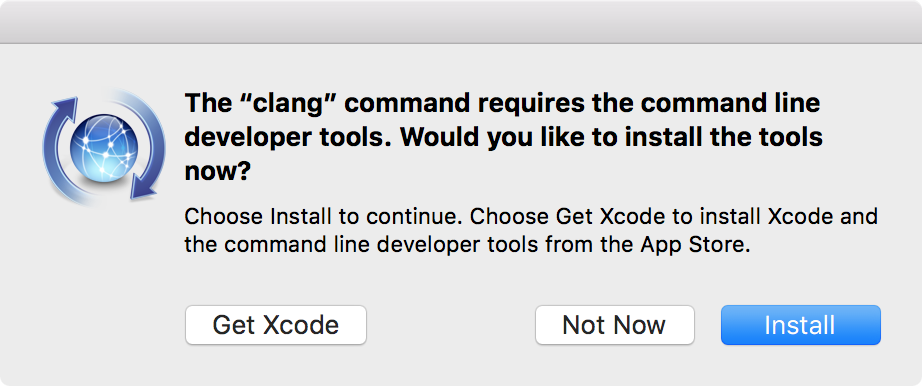
\includegraphics[scale=0.5]{fig/command-line-developer-tools.png}
  \caption{Command Line Developer Tools のインストールダイアログ}
  \label{fig:command-line-developer-tools}
\end{figure}

\begin{lstlisting}[language=bash]
$ clang
clang: error: no input files
\end{lstlisting}

\section{知っていると便利な macOS 特有のコマンド}

\chapter{configure と Make}
\label{chap:configure}

\section{\texttt{configure}を使った ROOT のコンパイル(非推奨)}
\label{sec:compile_configure}

最近のROOTでは非推奨もしくは全くサポートされていません\footnote{少なくとも6.16/00以降ではサポートされていません。}が、\texttt{configure}スクリプトと\texttt{make}コマンドを使ったROOTのビルドは、かつて標準的な手法でした。また同様の手法で多くのオープンソースソフトウェアをビルドすることもできますので、ここでは参考として\texttt{configure}と\texttt{make}を使ったビルド方法を紹介します。

まずは\texttt{CMake}の時と同様にROOTのソースコードを\texttt{/usr/local}に展開します。
\begin{lstlisting}[language=bash]
$ cd /usr/local
$ sudo tar zxvf ~/root_v6.12.06.source.tar.gz
\end{lstlisting}

次に\texttt{configure}スクリプトを実行します。このスクリプトは\texttt{CMake}や\texttt{CmakeLists.txt}と同様に、ソフトウェアのビルドに必要な情報を集約します。

\begin{lstlisting}[language=bash]
$ cd root-6.12.06
$ sudo ./configure
\end{lstlisting}

色々とターミナルに出力されますが、最後に次のような表示が出れば\texttt{configure}は成功です。もし何かしらのエラーが表示される場合、ROOTのビルドに必要な他のコマンドやライブラリがインストールされていないことが考えられます。表示されたエラーをよく読み、原因が何かを考えて対応しましょう。
\begin{lstlisting}[language=bash]
Enabled support for asimage, astiff, bonjour, builtin_afterimage, builtin_ftgl, builtin_freetype, builtin_gl2ps, builtin_glew, builtin_unuran, builtin_lz4, builtin_llvm, libcxx, cocoa, explicitlink, fink, fitsio, gviz, genvector, krb5, ldap, memstat, opengl, python, rpath, search_usrlocal, shared, sqlite, tmva, xml.

To build ROOT type:

   make 

******************************************************************************
* The classic configure/make method of building ROOT is now DEPRECATED in    *
* favor of the CMake one.                                                    *
* Refer to README/INSTALL file for updated instructions or visit the page    *
* https://root.cern.ch/building-root                                         *
******************************************************************************
\end{lstlisting}
6.12/06では、\texttt{configure}を使ったビルドは「DEPRECATED」(旧式で非推奨)であると表示されます。新しいROOTを使う場合は、節~\ref{subsec:compile_cmake}の\texttt{CMake}を使ったビルドを推奨します。

あとは、\texttt{CMake}のときと同様に\texttt{make}を実行します。
\begin{lstlisting}[language=bash]
$ sudo make -j8
\end{lstlisting}
うまくコンパイルが全て完了すると、次のような表示が最後に出るはずです。
\begin{lstlisting}
root [0] 
Processing hsimple.C...
hsimple   : Real Time =   0.07 seconds Cpu Time =   0.05 seconds
(TFile *) 0x7fb0fae560c0
 
   ============================================================
   ===                ROOT BUILD SUCCESSFUL.                ===
   === Run 'source bin/thisroot.[c]sh' before starting ROOT ===
   ============================================================
\end{lstlisting}

\texttt{make}実行時に何もオプションを渡さない場合、発展的な機能やマイナーな機能は「Enabled support」の一覧に入りません。\texttt{make}実行時に例えば次のようにオプションをつけることで、オプションもビルドすることができるようになります。

\begin{lstlisting}[language=bash]
$ sudo ./configure --enable-minuit2 --enable-gdml
\end{lstlisting}

\texttt{configure}を使った場合は展開したソースファイルのディレクトリ内でコンパイルを行いますので、次のような\texttt{\~{}/.bashrc}の設定になります。
\begin{NoFloat}
\lstinputlisting[language=bash]{src/bashrc.sh}
\end{NoFloat}

\section{configureとMakeの一般的な解説}

macOSやLinux環境でソフトウェアを導入する時、インストールの方法は主に3つあります。1つ目は、\ref{sec:Homebrew}で説明したようなパッケージ管理ソフト\footnote{macOSではMacPorts、Fink、Homebrewなど、LinuxではYumやAPTなど。}を使う方法す。2つ目は、既にコンパイル済みでバイナリ配布されているソフトを導入する方法です。例えば、KeyRemap4MacBookをインストーラを使ってインストールしたのがこれに当たります。また、ROOTを入れる場合でもバイナリ配布されているものを使うことが可能です。3つ目は、ソースコードの配布されているソフトウェアを自分でコンパイル(compile)する\footnote{ビルド(build)するとも言います。}方法です。これは\ref{sec:ROOT_install}でROOTの導入として説明しました。

自分でソフトウェアをソースコードからコンパイルする場合、標準的なやり方が存在します。また、研究で通常使うソフトウェアの多くがこの標準的な方法に則して作成されています。そのためここで説明する方法を覚えておけば、多くのソフトウェアを自分で簡単にインストールできるようになります。

このやり方を覚えるために、「GNU Hello\footnote{\url{http://www.gnu.org/software/hello/}}」と呼ばれるソフトウェアを試しにインストールしてみましょう。この「GNU Hello」は標準的な方法を学ぶ上で最適なもので、インストールしても実用性はありません。

まず、次のコマンドで\url{http://ftp.gnu.org/gnu/hello/}から最新版の\texttt{hello-2.8.tar.gz}を落としてきて展開します。展開されたディレクトリに移動して\texttt{ls}で中身を見てみましょう。

\begin{lstlisting}[language=bash]
$ curl -O http://ftp.gnu.org/gnu/hello/hello-2.8.tar.gz
  % Total    % Received % Xferd  Average Speed   Time    Time     Time  Current
                                 Dload  Upload   Total   Spent    Left  Speed
100  681k  100  681k    0     0   150k      0  0:00:04  0:00:04 --:--:--  166k
$ tar zxf hello-2.8.tar.gz
$ cd hello-2.8 
$ ls
ABOUT-NLS      INSTALL        THANKS         configure.ac   man
AUTHORS        Makefile.am    TODO           contrib        po
COPYING        Makefile.in    aclocal.m4     doc            src
ChangeLog      NEWS           build-aux      lib            tests
ChangeLog.O    README         config.in      m4
GNUmakefile    README-release configure      maint.mk
\end{lstlisting}

ここで重要なのは、\texttt{README}、\texttt{INSTALL}、\texttt{configure}の3つです。\texttt{README}は、そのソフトウェアに関する全般的な説明が書かれています。\texttt{INSTALL}には、そのソフトウェアのインストール方法が書かれています。\texttt{less}コマンドなどで、試しに中身を読んでみて下さい。

\begin{lstlisting}[language=bash]
$ less README
$ less INSTALL
\end{lstlisting}

\texttt{configure}はシェルスクリプトで、そのソフトウェアをコンパイルするときに必要なライブラリやコマンドが存在するかどうか、存在するパスはどこか、OSの環境は何かを自動的に調べて必要な設定をしてくれます。また、必要に応じてユーザが様々なオプションを指定することができます。どのようなオプションがあるかは、次のようにヘルプを表示することで読むことができます。

\begin{lstlisting}[language=bash]
$ ./configure --help
\end{lstlisting}

様々なオプションが表示されますが、このうち最も頻繁に使われるのがインストール先の指定のオプション\texttt{--prefix}です。次のように\texttt{configure}を実行することで、\texttt{hello}コマンドを\texttt{/usr/local/bin}にインストールし、またマニュアルを\texttt{/usr/local/share/man/man1}にインストールします。もし\texttt{/usr/local}の代わりに他の場所をしていすれば、これらのファイルは指定した場所の下にインストールされます。
\begin{lstlisting}[language=bash]
$ ./configure --prefix=/usr/local
\end{lstlisting} 

\texttt{configure}が問題なく実行されれば、\texttt{Makefile}というファイルが新たに生成されているはずです。このファイルの中には、そのソフトウェアをどのような手順でコンパイルすれば良いかが全て書かれています。ユーザはどのようなソースコードがあるのかなどを気にする必要はありません。この\texttt{Makefile}の手順の通りに自動的にソフトウェアをコンパイルするには、以下の
コマンドを打つだけです。

\begin{lstlisting}[language=bash]
$ make -j 4
\end{lstlisting} 

\texttt{make}コマンドが\texttt{Makefile}の中身を自動的に調べ、そこに書かれている手順を追ってコンパイルを行います。\texttt{-j 4}のオプションは、使っているCPU能力を最大限に引き出すためのものです。この場合、4コアのCPUを全て使ってくれます。

これで必要なファイルが全て生成されたので、最後にインストール作業を行います。通常は\texttt{/usr/local}にインストールする場合に管理者権限が必要なので、次のコマンドを実行します。

\begin{lstlisting}[language=bash]
$ sudo make install
Password:
\end{lstlisting}

これで、\texttt{/usr/local/bin/hello}などが配置されたはずです。では、確認のため\texttt{hello}を実行しましょう。 
\begin{lstlisting}[language=bash]
$ hello
Hello, world!
\end{lstlisting}

どのようなオプションを渡せるかは、\texttt{--help}や\texttt{-h}をつけて確認します。
\begin{lstlisting}[language=bash]
$ hello -h
Usage: hello [OPTION]...
Print a friendly, customizable greeting.

  -h, --help          display this help and exit
  -v, --version       display version information and exit

  -t, --traditional       use traditional greeting format
  -n, --next-generation   use next-generation greeting format
  -g, --greeting=TEXT     use TEXT as the greeting message

Report bugs to: bug-hello@gnu.org
GNU Hello home page: <http://www.gnu.org/software/hello/>
General help using GNU software: <http://www.gnu.org/gethelp/>
\end{lstlisting}

また\texttt{hello}コマンドのマニュアルを見るには\texttt{man}コマンドを使います。

\begin{lstlisting}[language=bash]
$ man hello
\end{lstlisting}

\chapter{本文で登場したROOTスクリプトのPyROOT版}
ここでは、本文中で登場したROOTスクリプトをPyROOTで書き換えた例を掲載します。\texttt{foo.C}というROOTスクリプトであれば、\texttt{foo.py}というPyROOTスクリプトにしてあります。

\begin{NoFloat}
\lstinputlisting[language=python,breaklines=true,caption=\texttt{population.py},label=code:population_py,numbers=left]{src/population.py}
\end{NoFloat}


\end{document}
